%%%%%%%%%%%%%%%%%% Environment
\documentclass[11pt]{article}
\usepackage[utf8]{inputenc}
%\documentclass{article}
%\usepackage{beamerarticle}

%%%%%%%%%%%%%%%%%% Basic Packages
\usepackage{amsbsy}
\usepackage{amstext}
\usepackage{amsfonts}
\usepackage{amssymb}
\usepackage{amsthm}
\usepackage{amsmath}
\usepackage{bbm}
\usepackage{color}
\usepackage{arydshln}
\usepackage{multirow}
\usepackage{changepage}
\usepackage{threeparttable,booktabs}
\usepackage{enumitem}
\usepackage{subfigure}
%\usepackage{natbib}
%\bibliographystyle{abbrvnat}
%\setcitestyle{authoryear,open={((},close={))}}

%%%%%%%%%%%%%%%%%% Style
\usepackage[margin=1in]{geometry}%
\usepackage[doublespacing]{setspace}
%\usepackage{setspace}
%\setstretch{1.618}
%%%%%%%%%%%%%%%%%% Fonts and Graphics
\usepackage[cjk]{kotex} %Korean TeX
\usepackage[pdftex]{graphicx}

%%%%%%%%%%%%%%%%%% Theorem
\newtheorem{Theorem}{Theorem}
\newtheorem{Lemma}{Lemma}
\newtheorem{assumption}{Assumption}
\newtheorem{prop}{Proposition}
\newtheorem{corollary}{Corollary}
\newcommand{\ju}{\textcolor{cyan}}
\newcommand{\yj}{\textcolor{magenta}}
\usepackage{apptools}
\AtAppendix{\counterwithin{Lemma}{section}}
\AtAppendix{\counterwithin{table}{section}}
\AtAppendix{\counterwithin{figure}{section}}

%%%%%%%%%%%%%%%%%% Bibliography and Appendices
%\usepackage[natbibapa]{apacite} % Including URLs in bibliography
\usepackage{natbib}
\usepackage[hyphens]{url} % Including URLs in bibliography
%\usepackage[toc,page,title]{appendix} % Extra control of appendices
\usepackage[titletoc,toc,title]{appendix}
\usepackage{chngcntr}

%%%%%%%%%%%%%%%%%Appendix title
\let\oldappendix\appendix
\makeatletter
\renewcommand{\appendix}{%
  \addtocontents{toc}{\let\protect\numberline\protect\appendixnumberline}%
  \renewcommand{\@seccntformat}[1]{Appendix~\csname the##1\endcsname\quad}%
  \oldappendix
}
\makeatother

%%%%%%%%%%%%%%%%%% Cover Page
\title{
	\onehalfspacing
	{\huge Sharing Economy in the Cloud:\\Pricing Schemes for Peer-to-Peer Storage Platforms}
}
\author{
	YoungJae Jang$^1$
	\and Jaeung Sim$^1$
	\and Kun Soo Park$^2$\thanks{Corresponding author. E-mail address: kunsoo@snu.ac.kr}
	\and Daegon Cho$^1$
}
\date{%
	\onehalfspacing
	$^1$KAIST College of Business, Seoul 02455, Republic of Korea\\%
	$^2$Seoul National University, Seoul 08825, Republic of Korea\\[2ex]%
	\today
}

%%%%%%%%%%%%%%%%%% Font Size of Abstract
\makeatletter
\renewenvironment{abstract}{%
	\if@twocolumn
	\section*{\abstractname}%
	\else %% <- here I've removed \small
	\begin{center}%
		{\bfseries \large\abstractname\vspace{\z@}}%  %% <- here I've added \Large
	\end{center}%
	\quotation
	\fi}
{\if@twocolumn\else\endquotation\fi}
\makeatother

%%%%%%%%%%%%%%%%%% Beginning of the Manuscript
\begin{document}
%
\begin{center}{\LARGE Sharing Economy in the Cloud:\\
Pricing Schemes for Peer-to-Peer Storage Platforms}\end{center}
%\maketitle
%
%
\begin{abstract}
	\onehalfspacing
	\noindent
	% The first page of the manuscript should include the title of the paper and an abstract of 100-250 words (POMS).
	{\normalsize
	% 2022-03-13 version (236 words)
	In response to an unprecedented surge in data storage demands, peer-to-peer (P2P) storage platforms with blockchain technology have emerged as a viable alternative to conventional cloud storage services. While crowdsourcing of unused storage resources in P2P storage platforms might be securely conducted with blockchain, the decentralized structure with peer contributions does not necessarily ensure sufficient storage availability. There are several incentive schemes that P2P storage platforms can employ to encourage users to participate in the platform for storage capacity and access; however, research has done little to provide a theoretical background for the effectiveness of pricing schemes in such an emerging service. This paper examines pricing schemes that P2P storage platforms can adopt: a two-part tariff, subscription, and hybrid pricing. Using a game-theoretic approach, we consider a profit-seeking platform by incorporating interplays among renters and providers and the platform's algorithmic decision under a given pricing scheme. We show that a two-part tariff maximizes short-run profits of the platform and providers, while subscription-based pricing shows the highest renter surplus. For the total surplus of all stakeholders, we find that the optimal pricing scheme differs by the size of potential providers. When there are enough providers to meet storage demand from renters, overall welfare is higher with subscription-based pricing that maximizes renters' welfare. However, we show that hybrid pricing or a two-part tariff maximizes social welfare in a situation wherein potential service providers are relatively scarce.}
\end{abstract}
\baselineskip 15pt
\hspace{0.2cm} {\sc Keywords:} Cloud computing; peer-to-peer markets; pricing schemes; sharing economy
%
%
%\clearpage

% POM Author Instructions (Length): The page limit for the manuscript, including the abstract and references, is 32 pages, 1.5 spaced in a size 11 font, and it should have one-inch margins on all four sides of the page. Each page of the manuscript should be numbered. In addition, some proofs, lemmas, supporting tables/figures, additional references, or any additional material, may be included in an e-companion. There is no page limit for the e-companion. A page limit is imposed because papers should focus on their main contribution and short papers are more likely to be read and cited.

%\linespread{5}
\onehalfspacing
%
%
\section{Introduction}\label{sec:intro}
Despite the rapid growth of public cloud services such as Amazon Web Services (AWS), the supply of storage capacity is expected to be insufficient to meet unprecedented demands of data volume in the near future. According to the International Data Corporation (IDC), the global spare storage capacity ratio in a commercial market was expected to be reduced from 33 percent in 2018 to 15 percent in 2020 \citep{robb2015space, idc2018worldwide}. As a prompt remedy for this upcoming shortage problem, a plausible solution might be the efficient use of available storage space scattered over billions of personal computers (PCs). The total non-commercial hard drive space on PCs is estimated to be nearly 250 exabytes (or 250,000 petabytes) globally, which is larger than the capacity of all public cloud services combined \citep{thompson2014cloud}.\footnote{In 2012, Facebook stored 100 petabytes (PB), Microsoft stored 300 PB, and Amazon held 900 PB of data in their respective cloud services.} If individual users can successfully share their under-utilized hard-drive spaces with potential renters, this could be a valuable complementary and competing service with conventional public cloud services. However, data storage sharing between PCs as a direct form of peer-to-peer (P2P) transactions has not been widely implemented for several notable reasons, such as information privacy and security concerns.

To adequately deal with these non-negligible issues, new data storage and sharing platforms integrating various Industry 4.0 technologies such as cloud computing and blockchain have been emerging \citep{protocol2017filecoin, vorick2014sia, wilkinson2016storj}. The blockchain-enabled decentralized P2P storage platforms make under-utilized hard-drive space available for data storage services with advanced encryption technology. Specifically, the P2P file-sharing protocol allows renters to store large files in fragmented pieces distributed to many individual providers. In this way, no single provider has enough fragments to reconstruct the original file. Also, the original files can be reassembled only by a renter’s private key, further ensuring that storage providers cannot read the content. In addition, the platforms use novel blockchain technology, by which storage contracts between renters and providers are recorded and verified collaboratively. Peers are incentivized or penalized based on their contributions to the network, leading to a stable resilience in the system.

While P2P storage services are still in beginning stages, they have already attracted significant attention in the cryptocurrency market with massive successes from initial coin offerings (ICOs). For instance, Storj, a platform that appeared in 2014, has already reached a market capitalization of \$391.0 million with a total storage capacity of 36.7 PB, 71,689 platform users, and 285 million files. Similarly, Sia has reached a market capitalization of \$872.9 million. It has a total 3.5PB storage capacity and 1.2 million accumulated downloads. Filecoin, which appeared relatively recently, set a new record in ICO funding of \$257 million in 2017 and currently ranks 24th among all cryptocurrencies with a market capitalization of \$6.816 billion. Surprisingly, it reached a total 629.3PB storage capacity within ten months from its service launch. These cases demonstrate the expectation that P2P file-sharing services will rapidly grow by successfully mitigating security issues with a blockchain-enabled decentralized approach.\footnote{Please refer to recent statistics of Storj, Sia, and Filecoin from https://www.storj.io/, https://siastats.info/, and https://file.app/, respectively. All statistics in this paragraph were observed on August 12, 2021.} At the same time, it raises question about attracting and securing greater numbers of participants to transition to the next stage.

In fact, decentralization creates an undesirable problem regarding storage availability. P2P platforms are not in control of storage capacity or online connection to stored files, so it is not easy to maintain and control agreeable service levels for both. In this regard, P2P storage platforms rely mainly on various economic incentives to attract and maintain providers to ensure sufficient levels of availability in terms of storage capacity and online connection to storage \citep{babich2020distributed, beck2018governance}. P2P platforms currently charge renters two-part fees: a storage service fee for providers sharing storage space with renters and a bandwidth service fee for maintaining providers' online connection to shared storage for renters. Sia, for example, has used a two-part tariff that imposes a base storage fee for using the storage capacity and a bandwidth fee for each download request for stored data. Storj charged the same type of fees for both services. Recently, Storj has introduced a new pricing scheme that provides free usage volume up to a certain threshold.\footnote{Storj's latest pricing policy is available at https://www.storj.io/pricing.} Once renters' download requests exceed this point, the platform begins imposing the bandwidth service fee. Although these platforms need to carefully design their pricing schemes to gather potential providers and renters effectively, little is known about the impact of possible pricing schemes on providers, renters, or platforms for this new and immature market. 

Thus motivated, this study aims to investigate a P2P storage platform's optimal design in terms of service fees, storage redundancy algorithms, and the implications of pricing schemes on profit and surplus. We incorporate pricing schemes that centralize public cloud services or that P2P storage platforms have adopted in practice. Specifically, P2P storage platforms have widely adopted a two-part tariff, while conventional public cloud services have widely used pay-per-use, subscription-based, and hybrid pricing \citep{kansal2014pricing}. We compare the effectiveness of these pricing schemes and their impacts on services, e.g., whether a specific pricing scheme that burdens renters for the provider's operating costs indeed brings benefits to the platform and whether the subscription-based scheme is appropriate for decentralized P2P storage services.

Specifically, we consider three pricing schemes: First, we investigate the two-part tariff (a lump-sum fee for the storage capacity + pay-per-use fee for the download bandwidth). Second, we incorporate subscription-based pricing, wherein renters gain unlimited free access to stored files after paying for storage capacity. Finally, we consider hybrid pricing, which provides a lump-sum fee for storage and a limited allowance of free bandwidth service and charges a pay-per-use fee for excess downloads. Regarding these pricing schemes, we intend to analyze their consequences on P2P storage services by answering the following research questions:
% \begin{itemize}
% 	\item How do the platform's optimal service fees change according to the pricing scheme?
% 	\item How should the platform decide its redundancy algorithm considering the pricing scheme and two-sided interactions?
% 	\item Which pricing scheme would the profit-seeking platform choose?
%     \item Which pricing scheme would maximize the overall system surplus?
% 	\item How does the impact of the pricing scheme change by the supply of sharing resources from potential providers?
% \end{itemize}
\textcolor{blue}{
\begin{itemize}
	\item How should the platform set its redundancy algorithm and service fees according to the pricing scheme?
    \item Which pricing scheme would maximize the platform's profit and the overall system surplus?
	\item How do the numbers of potential renters and providers in the two-sided market affect effectiveness of pricing schemes?
\end{itemize}
}

To answer these questions, we build a game-theoretic model of a profit-seeking P2P storage platform that intermediates amongst storage providers and renters. In our model, the P2P storage platform sets its redundancy algorithm and service fees within the given pricing scheme. Then, storage providers with heterogeneous operational costs decide whether to join this P2P storage platform and share their unused storage capacity with renters. Finally, storage renters with heterogeneous willingness to pay for the storage service determine whether to adopt the P2P storage platform. For completed transactions between providers and renters, the platform charges commission rates to make a profit. We assume that the operating cost incurred by a storage provider increases with bandwidth usage levels that vary across renters. In storing a renter's file, the platform uses a redundancy algorithm (a $k$-of-$m$ erasure coding scheme) that divides each file into $k$ fragments and assigns encrypted copies of these fragments to $m$ ($> k$) providers. Here, we define the redundancy rate as stored volume divided by original file volume, $m/k$. Thus, the platform can only satisfy storage demand up to participating providers' capacities, divided by the redundancy rate. Based on this model setting, we analyze the platform's choice of service fees under each pricing scheme and compare the platform's profit and the system surplus across the pricing schemes.

Our results suggest that the platform should set the redundancy algorithms minimizing providers' total operating costs for all pricing schemes. We also show that when the first-best prices---which maximize the platform's profit when the size of potential providers is sufficient---are applicable, the two-part tariff always maximizes the platform's profit and provider surplus, and hybrid pricing follows. Notably, we see that hybrid pricing yields the same outcomes when it offers a small amount of free-download volume. Regarding the renter surplus, subscription-based pricing is most effective because the gain of renters with a higher usage frequency exceeds the loss from renters leaving the service due to a high storage fee. Consequently, subscription-based pricing outperforms other pricing schemes regarding the total surplus.

Markedly, we find that the impacts of pricing schemes differ significantly when potential providers are relatively scarce. If the size of potential providers is insufficient to fulfill the storage demand, the platform's optimal fees are subject to market-clearing prices---which make supply and demand equivalent---instead of first-best prices. In this situation, subscription-based pricing does not necessarily generate the maximum total surplus. In other words, a two-part tariff and hybrid pricing can dominate the subscription-based pricing concerning the platform's profit and total surplus. 

We further validate our findings by examining how endogenous commission rates affect the results. We find that our main insights continue to hold when the platform determines commission rates endogenously, although the thresholds that enable first-best prices change accordingly. Moreover, we conduct numerical analyses with relaxing assumptions on renter heterogeneity and observe consistent results.

\section{Related Literature}\label{sec:literature}

\subsection{Pricing and Capacity Management in Centralized Cloud}
Our paper is closely related to the growing literature on centralized cloud platforms. Recently, there has been growing interest in studying pricing strategies and capacity management in various academic fields such as operations management, information systems, and marketing \citep{fazli2018effects, chen2019pricing, chen2021discount, li2018should, kansal2014pricing, arbabian2021capacity}. For instance, \citet{chen2019pricing} considered two pricing schemes in cloud platforms: the reservation-based scheme and the utilization-based scheme. The former ensures a certain number of instances during a contract term (similar to subscription-based pricing), while the latter charges customers based on realized demand (similar to pay-per-use). Considering a duopoly model wherein cloud platforms adopting different schemes compete for customers with heterogeneous usage, they found that customers with lower demand volatility would prefer the reservation-based scheme, whereas those with higher volatility would prefer the utilization-based scheme.

\citet{nunez2021leveraging} proposed pricing schemes for Infrastructure as a Service (IaaS) cloud services, aiming to manage slack capacity and low utilization of resources. They combined two types of served-instance (contract) and on-demand services and examined their effectiveness across different market conditions in terms of service rate, market size, and service reliability. \citet{fazli2018effects} examined how autoscaling, which allows firms to scale their computational load to match customer demand automatically, affects market entry decisions, equilibrium prices, profitability, and consumer surplus. They showed that autoscaling might alleviate price competition because it reduces uncertainty about demand and excessive computational capacities.

These studies have mainly focused on pricing schemes and their role in managing capacity in centralized cloud platforms. Despite the advances in this research stream, little research has examined the role of pricing schemes in capacity management in P2P cloud platforms. Considering that P2P services hinge on independent providers, pricing decisions affect not only service demand and utilization but also the supply level of providers. Thus, neglecting this two-sided aspect inhibits us substantially from understanding the impact of pricing schemes on P2P cloud platforms.

\subsection{P2P Sharing of Computing Resources}
This paper is also related to the literature on sharing platforms for computing resources. The vast majority of studies in this stream have focused on the mechanism design of P2P file-sharing networks \citep{antoniadis2004p2p, casadesus2010p2p, de2017quality, ghasemkhani2018contracting, golle2001incentives}. \citet{antoniadis2004p2p} conducted a numerical analysis to compare several incentive schemes and suggested that a simple fixed fee scheme, wherein all peers are required to share a standard number of files, can achieve a high level of network efficiency. \citet{de2017quality} studied how individual peers make sharing decisions under quality-of-service based pricing schemes. They showed that socially optimal behaviors are induced when a pricing scheme does not charge users for content requests, while profit maximization is achieved when a pricing scheme charges users for requesting content. \citet{ghasemkhani2018contracting} proposed a contracting scheme for a monopolistic P2P file-sharing network, in which the network compensates each contracted peer node for the supply of files. They investigated the optimal reward scheme for the profit-seeking P2P network regarding network structures, content availability, propagation delay, etc.

It is worth noting that this literature stream has concentrated on file-sharing platforms only. Although a variety of computing resources---such as storage capacity, CPU power, and internet bandwidth---have recently been shared in online markets \citep{dickson2019monetizing, sharma2020blockchain}, we are aware of no study that has examined sharing platforms for these resources.
 
\subsection{Sharing Economy and Online Platforms}
Several studies have examined the benefits of sharing idle resources through these platforms. For example, \citet{zervas2017rise} provided empirical evidence that Airbnb's entry lowered hotel prices which was beneficial for consumers. \citet{lee2018battle} demonstrated that Uber significantly reduces search costs for riders. While numerous studies have echoed the point that emerging sharing platforms are good for consumers \citep{einav2016peer, greenwood2017show}, some analytic studies have indicated that those platforms are not necessarily beneficial to consumers in the long term as they might increase product prices \citep{jiang2018collaborative, weber2016product}. \citet{tian2018effects} showed that a sharing platform tends to increase the retailer's share of the gross profit margin in the distribution channel.

Recent studies have suggested theoretical frameworks for pricing strategies in sharing platforms \citep{bai2019coordinating, benjaafar2019peer, cachon2017role, bimpikis2019spatial, taylor2018demand}. \citet{benjaafar2019peer} considered both profit-maximizing and social-welfare-maximizing platforms and compared their equilibrium outcomes. They found that the differences in social welfare between these platforms are relatively modest. \citet{cachon2017role} examined several pricing schemes, including surge pricing, for sharing platforms with self-scheduling providers. They found that surge pricing generally achieves near optimal profit and improves the surplus of providers and consumers as labor becomes expensive. \textcolor{blue}{Recently, \citet{zhang2022two} studied the effects of wage schemes, such as fixed commission rate, dynamic commission rate, and fixed wage, on competition between sharing platforms. They showed that the relative competitiveness between the supply and demand sides determines which wage scheme is more effective in facilitating profits for platforms and surpluses for consumers and workers.}

\subsection{Contributions to the Literature}

Our study is the first attempt to provide a theoretical framework for pricing in decentralized cloud platforms. Unlike centralized cloud services, P2P cloud platforms do not have direct control over service capacities and rely on independent providers with unused storage capacity. Therefore, their pricing decisions affect both customers' costs and service levels. We develop a model that accounts for this complexity by incorporating providers' service participating decisions, renters' service adoption decisions, and interactions between providers and renters.

Furthermore, we investigate the potential of the pricing scheme that P2P storage platforms have not yet explicitly implemented--- subscription-based pricing, which has been widely adopted in conventional public cloud services \citep{kansal2014pricing}. We show that the impacts of pricing schemes on the system surplus can change based on the relative number of potential providers compared to the storage demand from renters. When there is a sufficient number of potential providers, subscription-based pricing, which P2P storage platforms have neglected in practice, always produces the highest renter surplus and the highest system surplus. Interestingly, a two-part tariff or hybrid pricing can dominate subscription-based pricing regarding the platform's profit and total surplus when the number of potential suppliers is insufficient to satisfy storage demand.

In addition, we incorporate the platform's algorithmic decision into our framework by considering peer decisions of the supply and demand sides. We show that P2P platforms need to set their redundancy algorithms to minimize total operating costs of providers in the system, and interestingly, this algorithmic decision is independent of pricing schemes. These findings suggest that P2P storage platforms can improve their pricing strategies and redundancy algorithms separately, even though each decision affects providers and renters simultaneously.

Our study also extends the literature on P2P sharing of computing resources. Recently, emerging platforms have enabled sharing of various computing resources, such as storage capacity, CPU power, and internet bandwidth \citep{dickson2019monetizing, sharma2020blockchain}. However, no study has contributed to our understanding of sharing platforms for these resources. Unlike P2P file-sharing services, P2P storage sharing comprises the initial storage service and the subsequent bandwidth service. Thus, a two-part tariff consisting of a lump-sum charge (storage fee) and a per-unit charge (bandwidth fee) is widely adopted, in practice. Hence, the existing framework for file-sharing platforms, where consumers are satisfied once they receive appropriate files, cannot be directly applied. We expect that our framework for P2P cloud storage, which prior studies have not examined, can provide valuable insights for sharing services of various computing resources. 

Lastly, this study contributes to the literature on pricing for the sharing economy, in general. We show that pricing schemes that reward providers can improve the system surplus when potential suppliers are too scarce compared to consumers. In this situation, the impact of pricing schemes varies according to the degree of scarcity of suppliers. For instance, P2P delivery platforms that serve various regions in terms of numbers of sellers, deliverers, and consumers might offer different pricing schemes across regions according to the relative scarcity of sellers or deliverers compared to consumers to improve the surplus of overall stakeholders. \textcolor{blue}{Prior studies on pricing in the sharing economy, such as \citet{cachon2017role} and \citet{zhang2022two}, did not consider the potential of the pricing schemes that we have examined in this paper. Specifically, these studies postulated a common price and focused on price-wage relationships---i.e., how the platform should share its revenue with workers---rather than on how to price services depending on usage levels. Consequently, these studies paid scant attention to comparing service pricing schemes, such as two-part tariff, subscription-based pricing, and hybrid pricing.} In fact, a two-part tariff that consists of lump-sum fees and pay-per-use can also be used in other sharing platforms (e.g., base rates and cost-per-user in ride-sharing platforms). Hence, our model can extend these studies by enhancing insights on sharing platforms' pricing strategies.

Also, unlike \citet{cachon2017role}, we allow providers to have heterogeneous operating costs, which are also affected by renters' usage levels. Specifically, we postulate that individual providers have different sensitivities to their uptime levels and a higher usage level of a renter leads to a higher operating cost of a provider, which is not the typical model setting in the sharing economy literature. By incorporating this cost structure, we can examine the impact of providers' in-out decisions and the operational burden of bandwidth services.
%
%
\section{Model}\label{sec:model}

In this section, we first describe our model setups and players, followed by key decisions of players. We present the summary of basic notations in Table \ref{tbl:summary}. The proofs of all lemmas and theorems appear in Online Appendix \ref{app:proof}.

% \begin{table}[h] \centering
% \textbf{\caption{A Summary of Basic Notations\label{tbl:summary}}}
% \vspace{0.1in}
% \begin{tabular}{l | p{9cm}}
% \textbf{Notation} & \textbf{Description} \\ \hline
% $n_r$ & Number of potential renters \\
% $n_p$ & Number of potential providers \\
% $u_i$ & Renter $i$'s unit utility of bandwidth usage \\
% $\lambda_i$ & Renter $i$'s bandwidth usage \\
% $\rho_j$ & Provider $j$'s sensitivity to bandwidth provision\\
% $\theta$ & Redundancy rate \\
% $\xi$ & Unit operating cost\\
% $\alpha$ & Proportion of revenue that providers receive \\
% $p_s$ & Storage fee\\
% $p_b$ & Bandwidth fee
% \end{tabular}
% \end{table}



\begin{table}[h] \centering
\textbf{\caption{\textcolor{blue}{A Summary of Basic Notations}\label{tbl:summary}}}
\vspace{0.1in}
\begin{tabular}{l  p{14cm}}
\toprule
\textbf{Notation} & \textbf{Description} \\\hline
\multicolumn{2}{l}{\textbf{Parameters: Environment}}\\\hline
$n_r$ & Number of potential renters \\
$n_p$ & Number of potential providers \\
$\alpha$ & Proportion of revenue that providers receive \\\hline
\multicolumn{2}{l}{\textbf{Parameters: Heterogeneity}}\\\hline
$u_i$ & Renter $i$'s unit utility of bandwidth usage \\
$\lambda_i$ & Renter $i$'s bandwidth usage \\
$\rho_j$ & Provider $j$'s sensitivity to bandwidth provision\\\hline
\multicolumn{2}{l}{\textbf{Platform's decision variables}}\\\hline
$\theta$ & (Algorithm decision) Redundancy rate \\
$t$ & (Algorithm decision) Required uptime, determining unit operating cost $\xi$\\
$p_s$ & (Pricing decision) Storage fee\\
$p_b$ & (Pricing decision) Bandwidth fee\\\hline
\multicolumn{2}{l}{\textbf{Performance measures}}\\\hline
$\Pi$ & Platform's profit\\
TS & Total system surplus\\
\bottomrule
\end{tabular}
\end{table}

\subsection{Model Setups}\label{subsec:setups}

We consider a P2P storage platform wherein some peers provide their unused storage (hereafter, \textit{providers}) and other peers rent storage space and request downloading of stored files (hereafter, \textit{renters}). The platform offers two services to renters: \textit{i)} initial file storage (storage service), and \textit{ii)} access to stored files via a download request (bandwidth service). Once a renter requests storage space to save a file, a platform divides her file into $k$ fragments and assigns them to $m$ ($> k$) providers.\footnote{P2P storage platforms employ a $k$-of-$m$ erasure coding scheme, under which an original file is divided into $k$ shards, and the shards are re-coded into $m$ encrypted fragments ($m > k$) \citep{wilkinson2016storj}. Since any $k$ fragments among $m$ fragments are sufficient to reconstruct the file, erasure coding enables high reliability with low expansion factors \citep{weatherspoon2002erasure}. See Online Appendix \ref{app:algorithm} for technical details.} After completing the initial file storage, a renter can request a download of the stored file to the providers.

Since the availability of stored files to storage renters is critical for P2P storage services, the P2P storage platforms should make the likelihood of file transfer failure negligible. Therefore, the platform needs to carefully set the algorithmic parameters: 1) the redundancy in the erasure coding $\theta \equiv \frac{m}{k}$, which refers to the proportion of the size of the duplicated data compared to the size of the original data, and 2) uptime $t$, which represents the proportion of provider's time being connected to the P2P network \citep{protocol2017filecoin, vorick2014sia, wilkinson2016storj}. \textcolor{blue}{We postulate that the platform considers the algorithm parameter combinations that maintain the same failure probability. In doing so, the platform may increase $\theta$ and decrease $t$ or vice versa. When the platform decides to raise $\theta$ and correspondingly reduce $t$, participating renters have to pay higher storage costs due to the higher redundancy rate, while providers can mitigate their operating burden. Consequently, the P2P network imposes a higher burden on renters. On the other hand, when the platform meets the probability by increasing $t$ rather than $\theta$, providers have to bear higher operating costs due to higher bandwidth uptime.}

P2P storage platforms attempt to develop redundancy algorithms that ensure extremely low failure probabilities. Theoretically and practically, it has been shown to be extremely rare for well-performing P2P networks to experience file transfer failure in practice.\footnote{For instance, the failure probability of a $k$-of-$m$ erasure coding is 5.266e-10 wherein $k=6$, $m=18$, and $t=0.90$ \citep{wilkinson2016storj}. In Sia's storage network, providers must maintain a 95–98\% uptime, enabling the network to achieve 99.9999\% availability of stored files to renters. Online Appendix \ref{app:algorithm} provides more details on algorithmic backgrounds.} Thus, we assume that the P2P storage platform sets an availability goal that is sufficiently large and close to its upper bound, one, and only considers the $(\theta, t)$ combinations that satisfy this availability goal. As such, our model does not take the failure probability of the file transfer into account.

\begin{figure}[ht!]
\centering
\includegraphics[width=14cm]{fig1_timeline_minor_revision.pdf} 
\textbf{\caption{\textcolor{blue}{The Sequence of Events}\label{fig:timeline}}}
\end{figure}

Figure \ref{fig:timeline} illustrates the sequence of the events for the platform, providers, and renters in our model. \textcolor{blue}{Specifically, the platform observes the potential market size of peers ($n_r$ and $n_p$). In response to the \textit{exogenously} given market condition, pricing scheme, and commission rate, the platform first determines its redundancy algorithm ($\theta$, $t$). Then,} the platform sets its service fees $(p_s, p_b)$, which are consistent with the current market situation, wherein the development of a redundancy algorithm takes several months or years.\footnote{Sia and Storj have not officially changed their algorithms since their releases. Also, Sia has not adopted the 64-of-96 algorithm, which this platform announced its development plan in 2020. The announcement is available at https://blog.sia.tech/cloud-storage-for-2-tb-mo-8a34043e93bb.} After that, potential providers for this P2P storage service decide whether or not to join the platform based on their expected profits. Once a provider joins the platform, he provides unused storage spaces to renters. Lastly, observing service fees and the available storage capacity, potential renters of the P2P storage service evaluate its expected utility and decide whether to adopt it. Once the P2P storage service is adopted, a renter starts using the storage spaces from providers.

We now further explain three essential players in the P2P file-sharing service: renters, providers, and a service platform.

\textbf{\textit{Renters.}} We consider a renter that needs a storage space for her unit volume of files. We denote the total number of potential renters in the market by $n_r$. Each potential renter decides whether to adopt the P2P storage platform and rent the storage space from providers. If a renter adopts the platform, she will obtain the usage value and pay the storage service fees for storing files to the providers' spaces and the bandwidth service fees for requesting a download of stored files. The renters will join the platform if their usage value exceeds the total service costs.

This model concerns renters with a continuum of bandwidth usage level (or frequency of download requests) of stored files denoted by $\lambda$. It has been empirically observed in the literature that the usage of a cloud-resource is distributed with relatively heavy tails compared with exponential, log-normal, and normal distributions \citep{loboz2012cloud}, similarly to other digital resources like smartphone and YouTube usage \citep{falaki2010div, gill2008char}. Thus, we assume that a renter's bandwidth usage $\lambda$ follows the Pareto distribution in keeping with the extant literature \citep{bandi2015robust, li2018should, ramirez2017adapt}.

Based on this assumption, the probability distribution function of the bandwidth usage level can be expressed as $f(\lambda) = \frac{b \lambda_0^b}{\lambda^{b+1}}$, where the minimum bandwidth usage level is denoted by $\lambda_0$. For analytical tractability, we simplify our assumption such that the distribution of bandwidth usage level is characterized by the parameter value of $b = 2$. We also incorporate heterogeneous valuation of a renter's service usage. Specifically, we assume that renter $i$'s utility per unit volume of bandwidth usage (i.e., $u_i$) follows a uniform distribution; that is, $u_i \sim U[0, 1]$. As a result, renter $i$'s total utility obtained from storing files is $\lambda_i u_i$. To focus on the interplay among the platform, providers, and renters, we assume that $\lambda_i$ and $u_i$ are independent.

Renters pay the total service cost $c(p_s, p_b, \lambda_i)$ for their storage and bandwidth services according to the service fees ($p_s, p_b$) set by the P2P storage platform. This cost may change by $\lambda$ depending on a pricing scheme. As the utility per bandwidth volume $u_i$ is assumed to be bounded above and below by $0$ and $1$, the bandwidth service fee $p_b > 1$ will lead to a negative utility from the bandwidth for every renter. Thus, we restrict our attention to the case where the platform's bandwidth fee varies between $0$ and $1$, i.e., $p_b \le 1( = \bar{u})$.

\textbf{\textit{Providers.}} We consider $n_p$ potential providers who can share their unit volume of unused storage space. A provider will participate in the P2P storage platform if his expected revenue exceeds his operating costs. If a provider joins the P2P storage platform, he earns revenue based on the storage and bandwidth services he offers. The provider's revenue comes from the renters' payments for the service, subtracted by the platform's commission rates. We denote the proportion a provider receives from service fees imposed on renters by $\alpha \in [0, 1]$. Given that the storage fee applies to the provider's unit volume of space, the revenue for a provider's storage service is proportional to $\alpha p_s$ across all pricing schemes. In contrast, the revenue from a provider's bandwidth service may vary from $\alpha p_b$ depending on the pricing scheme. For example, if the platform provides a free allowance of bandwidth service, the bandwidth revenue is zero.

We incorporate heterogeneous operating costs of providers for sharing each provider's unit volume of unused space. The operating cost may comprise multiple sources, including the opportunity cost of using computing resources, obsolescence of the computing device, and Internet and electricity costs. This suggests that operating costs increase with received download requests as well as the providers' own uptime. We thus express the operating costs of providers as $\rho_j \hat{\omega}_b \xi(t)$. In this term, $\rho_j$ represents provider $j$'s sensitivity to the bandwidth provision. We assume that $\rho_j$ follows a uniform distribution; that is, $\rho_j \sim U[0, 1]$. $\hat{\omega}_b$ refers to the expected bandwidth volume for each provider.\footnote{We denote the total bandwidth volume of all participating providers by $\omega_b$.} Lastly, $\xi(t)$ is the unit operating cost for a provider and increasing in uptime $t$. Hereafter, for notational convenience, we omit $t$ in $\xi(t)$ denote this simply by $\xi$.

Also, we only consider the case wherein operating costs are non-negligible in a provider's in-out decision. Specifically, when $\xi$ is substantially small, the platform makes all potential providers join the network for all pricing schemes, preventing us from exploring the interplay between providers' and renters' decisions. Considering that profitability and operating costs are major concerns in online forums for P2P storage platforms, such conditions are unrealistic in practice.\footnote{The profitability and operating costs are widely discussed among Storj's official forum (https://forum.storj.io/) and other forum users (e.g., Reddit).} Therefore, we assume that $\xi$ is sufficiently large; technically, $\xi > \frac{3}{4}\alpha$.

\textbf{\textit{Platform.}} We consider a profit-seeking platform that gathers renters and providers in the common marketplace and enables encrypted contracts for storage sharing services between them. The P2P storage platform first sets the redundancy rate $\theta$ and the required uptime $t$. For a given $\theta$, the platform can assign renters to providers until the storage demand multiplied by $\theta$ reaches the total storage capacity.

Then, in response to the market situation, the platform determines service fees $p_s$ and $p_b$. The platform makes a profit by charging commission rates on completed transactions. For instance, Sia operates $\theta=3$ and $t=0.98$, and it charges 3.9\% of the commission rate on all successful storage contract payouts to P2P storage users. To focus on the characteristics of pricing schemes, we assume exogenously given commission rate ($1-\alpha$) in the first part of our analysis (Sections \ref{sec:analysis1} and \ref{sec:analysis2}). We will relax this assumption and consider endogenous selections of the algorithm and commission rate in Section \ref{sec:analysis3}.
 
In the P2P storage services, the size of storage space offered by providers and the size of space requested (by renters) determine overall service availability. In addition, the redundancy rate $\theta$ affects service availability since a higher redundancy $\theta$ decreases the available space to renters the platform can provide. Thus, it is critical for the P2P service platform whether the capacity of potential providers in the market divided by the redundancy (i.e., $n_p/\theta$) exceeds the potential storage demand (i.e., $n_r$). In Sections \ref{sec:analysis1} and \ref{sec:analysis2}, we consider two scenarios: 1) the case of a sufficient base of potential providers in the market, and 2) the case of an insufficient base of potential providers.

\subsection{Peer Decisions}\label{subsec:peers}
We describe peer decisions under a given platform's decision. Specifically, we consider a renter's decision to adopt the P2P storage service and a provider's decision to join the platform. Table \ref{tbl:volume} presents the summary of notations for \textcolor{blue}{intermediate variables, including  volume variables and peer utility}.

% \begin{table}[h] \centering
% \textbf{\caption{A Summary of Volume Notations\label{tbl:volume}}}
% \vspace{0.1in}
% \begin{tabular}{l | p{12cm}}
% \textbf{Notation} & \textbf{Description} \\ \hline
% $\upsilon_s$& Total storage volume of renters willing to adopt the platform \\
% $\upsilon_b$& Total bandwidth volume of renters willing to adopt the platform \\
% $\omega_s$ & Total storage volume of providers willing to join the platform\\
% $\omega_b$ & Total bandwidth volume of providers willing to join the platform  \\
% $\hat{\omega}_s$& Expected storage volume for each provider\\
% $\hat{\omega}_b$ & Expected bandwidth volume for each provider \\
% \end{tabular}
% \begin{tablenotes}
%   \small
%   \item Note. The following equations hold: $\upsilon_b = \upsilon_{bp} + \upsilon_{bf}$, $\omega_b = \omega_{bp} + \omega_{bf}$, $\hat{\omega}_b = \hat{\omega}_{bp} + \hat{\omega}_{bf}$, where the subscripts \textit{bp} and \textit{bf} indicate the paid bandwidth volume and the free (i.e., unpaid) bandwidth volume, respectively. 
% \end{tablenotes}
% \end{table}


\begin{table}[h] \small \centering
\textbf{\caption{\textcolor{blue}{A Summary of Intermediate Variable Notations}\label{tbl:volume}}}
\vspace{0.1in}
\begin{tabular}{c  c  c  p{10cm}}
\toprule
\textbf{Notation}  & \textbf{Peer} & \textbf{Unit}& \textbf{Description} \\ \hline
\multicolumn{4}{l}{\textbf{Volume notation}}\\ \hline
$\upsilon_s$ &\multirow{2}{*}{Renter}&\multirow{4}{*}{Total}& Total storage volume of renters willing to adopt the platform\\
$\upsilon_b$&&& Total bandwidth volume of renters willing to adopt the platform \\\cline{2-2}
$\omega_s$ &\multirow{4}{*}{Provider}&& Total storage volume of providers willing to join the platform\\
$\omega_b$  &&& Total bandwidth volume of providers willing to join the platform \\\cline{3-3}
$\hat{\omega}_s$&&\multirow{2}{*}{Individual}& Expected storage volume for each provider\\
$\hat{\omega}_b$ &&& Expected bandwidth volume for each provider\\\midrule
\multicolumn{4}{l}{\textbf{Peer utility}}\\\hline
$U_i$ & Renter & \multirow{2}{*}{Individual}& Renter $i$'s total utility\\\cline{2-2}
$\pi_j$&Provider&& Provider $j$'s profit\\
\bottomrule
\end{tabular}
\begin{tablenotes}
  \small
  \item Note. The following equations hold: $\upsilon_b = \upsilon_{bp} + \upsilon_{bf}$, $\omega_b = \omega_{bp} + \omega_{bf}$, $\hat{\omega}_b = \hat{\omega}_{bp} + \hat{\omega}_{bf}$, where the subscripts \textit{bp} and \textit{bf} indicate the paid bandwidth volume and the free (i.e., unpaid) bandwidth volume, respectively. 
\end{tablenotes}
\end{table}

\subsubsection{A Renter's Decision} Renter $i$ decides to adopt the P2P storage service if the expected utility $U_i = \lambda_i u_i - c(p_s, p_b, \lambda_i)$ is higher than or equal to zero, wherein $c(p_s, p_b, \lambda_i)$ indicates the total service cost. Since a renter's service cost structure differs across pricing schemes, we provide the total storage and bandwidth volumes for each scheme. For simplicity, we denote a two-part tariff, subscription-based pricing, and hybrid pricing by superscripts $T$, $S$, and $H$, respectively.
 
\textbf{\textit{Two-part Tariff.}} In this pricing scheme, the platform charges renters the lump-sum storage fee $p_s$ for using storage space and the pay-per-use bandwidth fee $p_b$ for each download request (the unit bandwidth volume) to the stored files. In the two-part tariff, the total service cost of renter $i$ for the P2P storage service is expressed as $c(p_s, p_b, \lambda_i) = \theta p_s + \lambda_i p_b $. In this cost, $\theta p_s$ represents the storage service cost with the redundancy rate $\theta$, whereas $\lambda_i p_b$ refers to the bandwidth service cost with the bandwidth usage level $\lambda_i$. The utility of renter $i$ is then represented as $U_i = \lambda_i u_i - \theta p_s - \lambda_i p_b$.

We define $u^T(\lambda) \equiv \frac{\theta p_s}{\lambda} + p_b$, which indicates the lower bound of $u_i$ for renters who adopt the service with given bandwidth usage level $\lambda$ in the two-part tariff. Then, renter $i$ would adopt the platform if and only if $u_i \ge u^T(\lambda)$. Considering the distribution function of renters' bandwidth usage levels $\lambda$, we obtain the total expected storage demand and bandwidth demand from renters in the two-part tariff, denoted by $\upsilon_s^T$ and $\upsilon_b^T$, as:
\begin{equation*}
\begin{aligned}
&\upsilon_s^T = \int_{\max\{\lambda_0, \lambda^T\}}^{\infty} \{1-u^T(\lambda)\} f(\lambda) d \lambda,\\
&\upsilon_{b}^T = \int_{\max\{\lambda_0, \lambda^T\}}^{\infty} \{1-u^T(\lambda)\} \lambda f(\lambda) d \lambda \; (=\upsilon_{bp}^T),\\
&\text{where } \lambda^T = \frac{\theta p_s}{1-p_b}.
%&\upsilon_{bf}^T = 0\\
\end{aligned}
\end{equation*}
We also note that the free download volume of the bandwidth service $\upsilon_{bf}^T$ is zero because the platform does not offer the free bandwidth allowance in the two-part tariff.

\textbf{\textit{Subscription-based Pricing.}} When the platform adopts subscription-based pricing, it charges only a lump-sum fee for the storage service and offers the bandwidth service for free. Therefore, regardless of service usage level $\lambda$, renter $i$'s total service cost only consists of the storage fee multiplied by the redundancy rate (i.e., $c(p_s, p_b, \lambda_i) = \theta p_s$). Then, renter $i$'s utility is expressed as $U_i = \lambda_i u_i - \theta p_s$. Similarly to $u^T(\lambda)$, we define $u^S(\lambda) = \frac{\theta p_s }{\lambda}$ as the lowest $u_i$ of renters that adopt the P2P storage service for a given bandwidth usage level $\lambda$ under subscription-based pricing. The expected total storage demand and bandwidth demand from renters with respect to renters' $\lambda$, which is denoted by $\upsilon_s^S$ and $\upsilon_b^S$ is expressed as:
\begin{equation*}
\begin{aligned}
&\upsilon_s^S = \int_{\max\{\lambda_0, \lambda^S\}}^{\infty} \{1-u^S(\lambda)\} f(\lambda) d \lambda, \\
&\upsilon_{b}^S = \int_{\max\{\lambda_0, \lambda^S\}}^{\infty} \{1-u^S(\lambda)\} \lambda f(\lambda) d \lambda \; (=\upsilon_{bf}^S),\\
%&\upsilon_{bp}^S = 0\\
&\text{where } \lambda^S = \theta p_s.
\end{aligned}
\end{equation*}
Since the platform does not charge renters the bandwidth fee for the download volume of stored files, providers are not compensated for offering the bandwidth service. Accordingly, we have $\upsilon_{bp}^S = 0$.

\textbf{\textit{Hybrid Pricing.}} Under hybrid pricing, the platform charges the storage fee $p_s$ and offers a free bandwidth allowance up to $q \lambda_0$, where $\lambda_0$ represents the minimum bandwidth usage level among all potential renters, and $q\, (\ge 0)$ refers to a coefficient of the free bandwidth allowance. Note that $q = 0$ makes the hybrid pricing equivalent to the two-part tariff. The platform charges the bandwidth fee $p_b$ for the bandwidth usage that exceeds $q \lambda_0$. Therefore, renter $i$'s service cost is calculated as $c(p_s, p_b, \lambda_i) = \theta p_s + \max\{\lambda_i - q \lambda_0, 0\} p_b$, and her utility is $U_i = \lambda_i u_i - \theta p_s - \max\{\lambda_i - q \lambda_0, 0\} p_b$. For the hybrid pricing, we define $u^H(\lambda) \equiv \frac{\theta p_s +\max\{\lambda - q \lambda_0, 0\} p_b}{\lambda}$ as the lowest $u_i$ among renters who have a bandwidth usage level $\lambda$ and adopt the P2P storage service.

The characteristics of hybrid pricing substantially differ depending on the amount of the free bandwidth service $q \lambda_0$. Hereafter, we denote the hybrid pricing with $0 \le q \le 1$ and $q \ge 1$ by superscripts $Hl$ and $Hh$, respectively. When $0 \le q \le 1$, all renters that adopt the service have bandwidth usage levels higher than $q \lambda_0$. Thus, each renter will pay the bandwidth fee for bandwidth usage exceeding the free bandwidth allowance, where total bandwidth usage that is subject to bandwidth service cost is $\lambda_i - q \lambda_0$. As a result, $\upsilon_s^{Hl}$, $\upsilon_{bf}^{Hl}$, and $\upsilon_{bp}^{Hl}$ in hybrid pricing with low $q$ (i.e., $q\in [0,1]$) are expressed as:
\begin{equation*}
\begin{aligned}
&\upsilon_s^{Hl} = \int_{\max\{\lambda_0, \lambda^H\}}^{\infty} \{1-u^H(\lambda)\} f(\lambda) d \lambda, \\
&\upsilon_{bf}^{Hl} = \int_{\max\{\lambda_0, \lambda^H\}}^{\infty} \{1-u^H(\lambda)\} q \lambda_0  f(\lambda) d \lambda,\\
&\upsilon_{bp}^{Hl} = \int_{\max\{\lambda_0, \lambda^H\}}^{\infty}  \{1-u^H(\lambda)\} (\lambda - q \lambda_0) f(\lambda) d \lambda,\\
&\text{where } \lambda^H = \frac{\theta p_s - q \lambda_0 p_b}{1 - p_b}.
\end{aligned}
\end{equation*}
In contrast, when $q \ge 1$, some renters that adopt the service may use a bandwidth usage level lower than $q\lambda_0$. These renters will only pay the storage service fee, just as in the case of subscription-based pricing. Other renters pay the bandwidth service cost for a bandwidth usage level that exceeds the free bandwidth allowance, i.e.,  $\lambda_i - q \lambda_0$. Accordingly, $\upsilon_s^{Hh}$, $\upsilon_{bf}^{Hh}$, and $\upsilon_{bp}^{Hh}$ under hybrid pricing with high $q$ (i.e., $q\ge 1$) are calculated as below:
\begin{equation*}
\begin{aligned}
&\upsilon_s^{Hh} = \int_{\min\{q \lambda_0, \max\{\lambda_0, \lambda^S\}\}}^{q \lambda_0} \{1-u^S(\lambda)\} f(\lambda) d \lambda + \int_{\max\{q \lambda_0, \lambda^H\}}^{\infty} \{1-u^H(\lambda)\} f(\lambda) d \lambda, \\
&\upsilon_{bf}^{Hh} = \int_{\min\{q \lambda_0, \max\{\lambda_0, \lambda^S\}\}}^{q \lambda_0} \{1-u^S(\lambda)\} \lambda f(\lambda) d \lambda + \int_{\max\{q \lambda_0, \lambda^H\}}^{\infty} \{1-u^H(\lambda)\} q \lambda_0 f(\lambda) d \lambda,\\
&\upsilon_{bp}^{Hh} =  \int_{\max\{q \lambda_0, \lambda^H\}}^{\infty}  \{1-u^H(\lambda)\} (\lambda - q \lambda_0)f(\lambda) d \lambda.
\end{aligned}
\end{equation*}

\subsubsection{A Provider's Decision}

Each provider determines whether to offer his unused storage to renters through the platform. Depending on the platform's decision and market conditions, storage space from participating providers and storage demand from renters vary. If storage capacity offered exceeds the storage demand requested, we assume that the platform randomly assigns renters to providers, and providers equally share the total storage demand accordingly. Note that every provider holds a certain piece of a file due to the P2P storage platform's redundancy algorithm (see Online Appendix \ref{app:algorithm} for details). Thus, all providers can make positive revenues even if there are fewer renters than providers. Otherwise, if the potential capacity offered is insufficient to the storage demand from providers, we assume that storage demand is randomly rationed. That is, some demand is not served while all providers fully utilize their capacities. In sum, the expected storage volume for each provider $\hat \omega_s$ is expressed as:
\begin{equation*}
    \hat \omega_s = \frac{\min\{\theta \upsilon_s, \omega_s\}}{\omega_s},
\end{equation*}
where $\upsilon_s$ denotes total storage demand from renters who are willing to adopt the P2P storage service, and $\omega_s$ refers to total storage space of providers willing to join the platform. In this equation, $\min\{\theta \upsilon_s, \omega_s\}$ implies the total volume of shared storage. \textcolor{blue}{\textbf{Figure \ref{fig:illustration}} presents the conceptual illustration of potential peers ($n_r$ and $n_p$) and active participants.} Specifically, when there are sufficient participating providers \textcolor{blue}{(i.e., $\theta \upsilon_s \le \omega_s$)}, all renters can store their files in the network. Thus, $\theta \upsilon_s$ is identical to the total stored volume. In contrast, when the storage capacity of participating providers is insufficient to meet the demand \textcolor{blue}{(i.e., $\theta \upsilon_s > \omega_s$)}, the platform can serve storage up to $\omega_s$. In this case, the platform serves the renter's demand until $\omega_s / \theta$, which is the total storage capacity divided by the redundancy ratio.

\begin{figure}[ht!]
\centering
\includegraphics[width=16cm]{figure_potential_peers.pdf} 
\textbf{\caption{\textcolor{blue}{Illustration of Potential and Active Peers (when $n_r > n_p$)}\label{fig:illustration}}}
\end{figure}

Next, bandwidth volume, which affects the bandwidth revenue and operating cost, is determined. Bandwidth revenue comes from the amount of paid bandwidth volume $\hat{\omega}_{bp}$, which is proportional to $\hat{\omega}_s$ due to randomly rationing renters. The bandwidth cost comes from the provider's operating cost, which depends on the total bandwidth volume $\hat{\omega}_b$ that includes both free and paid amounts. Note that $\hat{\omega}_b > \hat{\omega}_{bp}$ holds when the platform offers a certain amount of free access to stored files under subscription-based pricing and hybrid pricing. Based on expected demand for the storage service and bandwidth service, we derive provider $j$'s profit $\pi_j$ as follows:
%%%%%%%%%%%%%%%%%%%%%%%%%%%
\begin{equation*}
	\begin{aligned}
	    &\pi_j =\alpha (\hat{\omega}_s p_s + \hat{\omega}_{bp} p_b) - \rho_j \hat{\omega}_b \xi,\\
	    &\text{where } \hat \omega_{bp} = \frac{\hat \omega_s}{\theta \upsilon_s} \cdot \upsilon_{bp}\text{ and } \hat \omega_b = \frac{\hat \omega_s}{\theta \upsilon_s} \cdot \upsilon_b.
    \end{aligned}
\end{equation*}

Here, $\hat \omega_s / (\theta \upsilon_s)$ implies that the platform assigns bandwidth volume to each provider proportionally to his share from the entire stored volume. In other words, each provider obtains a smaller portion of storage and bandwidth volumes as more providers join the platform.\footnote{\textcolor{blue}{Here are numerical examples of how volume notations are related to each other. Suppose that under a certain pricing scheme, service fees, and redundancy rate $\theta=3$, the total storage demand of renters is $\upsilon_s = 20$ and the total bandwidth demand is $\upsilon_b = 30$. Since providers need to store replicated shards of the original files, the required capacity to meet the storage demand is $3 \times 20 = 60.$}

\textcolor{blue}{Then, we consider two scenarios: 1) $\omega_s = 40$ and 2) $\omega_s = 80$. In the first scenario, the total storage capacity that providers are willing to offer is smaller than the required capacity; that is, $\theta \upsilon_s = 3 \times 20 > \omega_s = 40$. Thus, this network can retain the storage volume at best their capacity $\omega_s = 40$. Considering that each provider offers the unit volume of storage, and thus $\omega_s$ is equivalent to the number of participating providers, each provider will use his storage by $\hat{\omega}_s = \min\{3 \times 20, 40\}/40 = 1$. Consequently, each provider serves the bandwidth service proportionally to the ratio of its stored space $\hat{\omega}_s = 1$ to the required capacity to meet the entire storage demand $\theta \upsilon_s = 60$; that is, $\hat{\omega}_b = (\hat{\omega}_s/\theta \upsilon_s)\cdot\upsilon_b = (1/60)\times30 = 0.5$.}

\textcolor{blue}{In the second scenario, the total capacity that providers are willing to offer is greater than the required capacity; that is, $\theta \upsilon_s = 3 \times 20 < \omega_s = 80$. Hence, the network can bear all storage demand, and each provider's storage usage is calculated as $\hat{\omega}_s = \min\{3 \times 20, 80\}/80 = 0.75$. As a result, each provider bears the bandwidth volume by $\hat{\omega}_b = (0.75/60)\times30 = 0.375$.}}

Although storage volume and bandwidth volume are utilized homogeneously across providers, participation decisions can vary because sensitivity to the bandwidth provision $\rho_j$ is heterogeneous (i.e., $\rho_j \sim U[0, 1]$ as assumed above). For ease of interpretation, we define the threshold of the sensitivity to the bandwidth provision as $\rho_m$, wherein only the providers with their sensitivities lower than the threshold would participate in the P2P storage platform (i.e., provider $j$ joins the platform if and only if $\rho_j \le \rho_m$). Lemma \ref{lem:pvd_chr} presents providers' participation decisions to the P2P storage platform.

\begin{Lemma}\label{lem:pvd_chr}
For a given service fee ($p_s, p_b$), the total storage demand $\upsilon_s$, the total bandwidth demand $\upsilon_b$, and the total paid bandwidth demand $\upsilon_{bp}$, the threshold sensitivity $\rho_m$ and the expected storage volume for each provider $\hat{\omega}_s$ are determined as:
\begin{alignat*}{2}
        &\text{When } n_p \ge \theta \upsilon_s           &&\text{When } n_p < \theta \upsilon_s\\
        &(\rho_m, \hat{\omega}_s) = \begin{cases}
        (\frac{\tilde{\pi}}{g_1}, 1) &\text{if } \tilde{\pi} < g_2\\
        (\frac{\tilde{\pi}}{g_1}, \frac{g_2}{\tilde{\pi}}) &\text{if } g_2 \le \tilde{\pi} < g_1 \indent\\
        (1, \frac{g_2}{g_1}) &\text{if } \tilde{\pi} \ge g_1
        \end{cases}         &&(\rho_m, \hat{\omega}_s) = \begin{cases}
        (\frac{\tilde{\pi}}{g_1}, 1) &\text{if } \tilde{\pi} < g_1\\
        (1, 1) &\text{if } \tilde{\pi} \ge g_1
        \end{cases}\\ 
        &\text{where } \tilde{\pi} = \alpha(p_s + \frac{\upsilon_{bp}}{\theta \upsilon_s} p_b), g_1 = \frac{\upsilon_b}{\theta \upsilon_s}\xi \text{ and } g_2 = \frac{\upsilon_b}{n_p}\xi.
\end{alignat*}
\end{Lemma}

In this lemma, $\tilde{\pi}$ is revenue for each provider sharing the unit storage capacity; $g_1$ and $g_2$ are proportional to operating costs. The results suggest that all providers participate in the P2P network if the expected revenue is sufficiently larger than operating costs ($\tilde{\pi} \ge g_1$), and some providers begin to give up participation as costs exceed revenues ($\tilde{\pi} < g_1$). Here, both $\tilde{\pi}$ and $g_1$ decrease with the amount of shared storage $\theta \upsilon_s$, suggesting that a larger number of participating providers reduce not only each provider's revenue but also operating costs.

Notably, expected storage volume \textcolor{blue}{$\hat{\omega}_s$} differs by the number of potential providers $n_p$. When the storage capacity of potential providers is greater than storage demand (i.e., $n_p \ge \theta \upsilon_s$), the provider's capacity is partially utilized unless the expected revenue is too low (i.e., $\tilde{\pi} < g_2$). In contrast, when the storage capacity of potential providers is smaller than storage demand (i.e., $n_p < \theta \upsilon_s$), providers utilize their full capacity to serve renters.

\section{Optimal Decisions}\label{sec:analysis1}

We consider a P2P storage service platform whose objective is to maximize expected profit. \textcolor{blue}{As described in Figure \ref{fig:timeline}, the platform observes the potential renter (provider) size $n_r (n_p)$. Then, it sets its redundancy algorithm that maximizes expected profit under the given pricing scheme and commission rate. After that,} the platform determines its service fees ($p_s, p_b$) based on expected behaviors of renters and providers. \textcolor{blue}{Utilizing the volume notations (e.g., $\upsilon_s$, $\upsilon_b$, $\omega_s$ and $\omega_b$) describing intermediary variables induced by algorithm ($\theta, t$) and service fee ($p_s, p_b$) decisions in Section \ref{subsec:peers}}, we can express the platform's pricing decisions as the following optimization problem:
\begin{equation*}
    \begin{aligned}
        &\max_{p_s, p_b}~ \Pi(p_s, p_b) = (1-\alpha) (V_s p_s + V_{bp} p_b),\\
        &\text{ where  } V_{bp} = \frac{V_s}{\theta \upsilon_s} \cdot \upsilon_{bp} \text{ and } V_s = \min\{\theta \upsilon_s, \omega_s\}.
    \end{aligned}
\end{equation*}
Here, $V_s$ is the total volume of shared storage and $V_s / (\theta \upsilon_s)$ means the share of stored data from total storage demand. When there are sufficient participating providers, $V_s = \theta \upsilon_s$ and $V_{bp} = \upsilon_{bp}$. Otherwise, $V_s = \omega_s$ and $V_{bp} = (\omega_s / \theta \upsilon_s) \cdot \upsilon_{bp} < \upsilon_{bp}$, indicating that the total paid bandwidth volume is smaller than bandwidth demand.

Importantly, in the second scenario (i.e., $V_s = \omega_s$), the platform can always increase its profit by raising service fees. This is because the platform can attract a larger number of providers and serve more storage volume. For this reason, we can reduce this platform's problem into the equivalent problem as follows:
\begin{equation*}
    \begin{aligned}
        &\max_{p_s, p_b}~ \Pi(p_s, p_b) = (1-\alpha) (\theta \upsilon_s p_s + \upsilon_{bp} p_b)\\
        &\text{  s.t.  } \theta \upsilon_s \le \omega_s.
    \end{aligned}
\end{equation*}
This implies that maximum profit is achieved when the platform can afford all renters willing to adopt it. Hence, the platform should set service fees that can maintain the capacity of the participating providers $\omega_s$ higher than or equal to the required storage volume from renters $\theta \upsilon_s$.

In the following subsections, we first examine the platform's pricing decisions and then analyze the optimal redundancy algorithm. In examining pricing decisions, we consider two supply-side scenarios: 1) a market with a sufficient number of potential providers to fully satisfy renters' storage demand (hereafter, \textit{first-best prices)}, and 2) a market wherein renters are rationed by supply level due to an insufficient number of potential providers (henceforth, \textit{market-clearing prices}). Figure \ref{fig:taxonomy} illustrates the taxonomy of pricing schemes and pricing decisions. For each of the first-best prices and market-clearing prices, we examine the optimal service fees for the three pricing schemes we study in this paper. After obtaining optimal pricing decisions, we revisit the algorithmic decision and corresponding profit.

\begin{figure}[ht!]
\centering
\includegraphics[width=14cm]{old_figure/fig2_pricing_taxonomy.pdf} 
\textbf{\caption{Taxonomy of Pricing Schemes and Pricing Decisions\label{fig:taxonomy}}}
\end{figure}

\subsection{Optimal Service Fees}

\subsubsection{First-best Prices}

We define the first-best prices of service fees ($p_s, p_b$) as service fees that maximize the platform's profit when the number of potential providers is sufficient to meet storage demand from renters. In other words, this implies that the platform finds such service fees optimal for its profit when it does not have to be concerned about the availability of the storage capacity from potential providers in the market. We analyze and compare the optimal service fees for each of the three pricing schemes we consider in this paper. Using the derived renters' and providers' decisions in Section \ref{sec:model}, we obtain the optimal service fees for each pricing scheme in the first-best prices as shown in Lemma \ref{lem:pricing}.

\begin{Lemma}\label{lem:pricing}
For each pricing scheme, the first-best prices of the P2P storage platform results in the optimal service fees as below:
\begin{equation*}
    \left(p_s^o, p_b^o\right) = \begin{cases}
    \left(0, \frac{1}{2}\right) &\text{for the two-part tariff},\\
    \left(\frac{q \lambda_0}{2\theta}, \frac{1}{2} \right) &\text{for the hybrid pricing with } q \in [0,1],\\
    \left(\frac{3q(2q^2 - 1)}{2(4q^3-1)} \frac{\lambda_0}{\theta}, \frac{3q^2(2q-1)}{2(4q^3-1)}\right) &\text{for the hybrid pricing with } q\ge 1,\\
    \left(\frac{3 \lambda_0}{4\theta}, -\right) &\text{for the subscription-based pricing}.
    \end{cases}
\end{equation*}
Also, the optimal $p_s^o$ ($p_b^o$) is strictly (weakly) increasing in $q$.
\end{Lemma}

\begin{figure}[ht!]
\centering
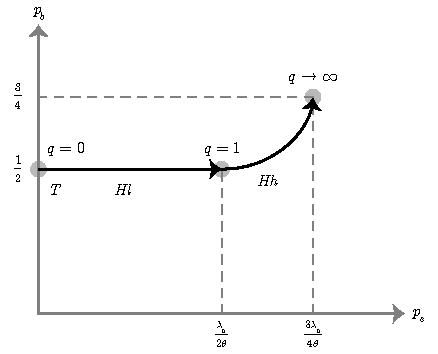
\includegraphics[width = 9cm]{old_figure/fig3_price_v2.pdf}
%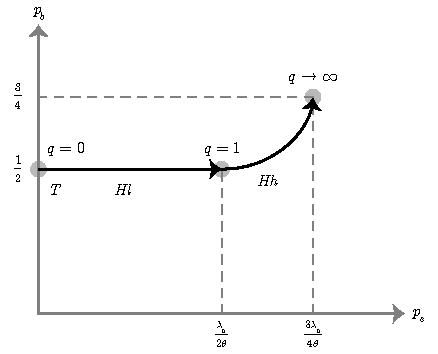
\includegraphics[scale=1.4]{old_figure/fig3_price_v2.pdf}
%\includegraphics[width=11cm]{fig3_price_v1.pdf} 
\textbf{\caption{Pricing Schemes and First-best Prices\label{fig:price}}}
\end{figure}

From this lemma, we derive how the optimal service fees of the profit-maximizing platform change according to each pricing scheme, which can be understood as the price structure with different amounts of the free bandwidth allowance. Figure 3 illustrates how optimal fees in first-best prices ($p_s^o, p_b^o$) change as the coefficient of the free bandwidth $q$ increases. 

First, we find that under a two-part tariff, the platform achieves the highest profit when it does not impose the storage fee (i.e., $p_s=0$) and charges the smallest bandwidth fee without any free amount of bandwidth service. Since all bandwidth usage is subject to bandwidth service fee under a two-part tariff, the platform is better off allowing renters to join the platform for free.

Second, when free bandwidth amount increases (i.e., $q$ increases) for $0 \le q \le 1$, the platform's optimal service fees are achieved by increasing the storage service fee while keeping the same bandwidth service fee. This occurs when the platform offers a free-download volume below the lowest bandwidth usage level of all renters $\lambda_0$. That is, all potential renters have a higher $\lambda$ than the free bandwidth allowance and are subject to the bandwidth service fee. In this vein, the platform can exactly make up for the revenue loss by offering free downloads and increasing a lump-sum fee. As a result, all renters pay the same total service cost in this pricing scheme, as is the case with a two-part tariff.

Lastly, the platform is better off increasing $p_b$ as well as $p_s$ when the amount of free download exceeds the minimum usage $\lambda_0$, i.e., $q \in (1, \infty)$. Specifically, $q > 1$ implies that some renters enjoy the complete bandwidth service for free because their bandwidth usage levels are lower than $q \lambda_0$. Then, the platform wants to fill this cost-utility gap by increasing the storage service fee to renters. Note that hybrid pricing becomes equivalent to subscription-based pricing when $q \rightarrow \infty$ because all renters can use the bandwidth for free.

\subsubsection{Market-clearing Prices}

Now, we consider the situation wherein renters are rationed by the supply level due to an insufficient number of potential providers in the market compared to the storage demand from renters (i.e., \textit{market-clearing prices}). We investigate how this supply-side restriction affects the platform's profit and system surplus for the three pricing schemes that we study in this paper.

To do so, we first investigate the required number of providers for first-best prices. Lemma \ref{lem:threshold} summarizes this result. 

\begin{Lemma}\label{lem:threshold}
The platform's optimal service fees belong to market-clearing prices when the number of potential providers $n_p$ is lower than the threshold $\psi$, which is calculated as:

\begin{equation*}
\begin{aligned}
    &\psi = \begin{cases}
    \frac{\xi \theta }{\alpha} n_r  &\text{ for the two-part tariff and the hybrid pricing with } q\le 1,\\
    \frac{5q^3 -3 q^2 + 3q - 2}{3q^3 + 3q^2 - 3q} \frac{\xi \theta }{\alpha} n_r   &\text{ for the hybrid pricing with } q \ge 1,\\
    \frac{5}{3}\frac{\xi \theta }{\alpha} n_r &\text{ for the subscription-based pricing,}
    \end{cases}
    \end{aligned}
\end{equation*}
and the optimal service fees of the platform decrease in $n_p$ when $n_p \le \psi$. 
\end{Lemma}

\begin{figure}[ht!]
\centering
%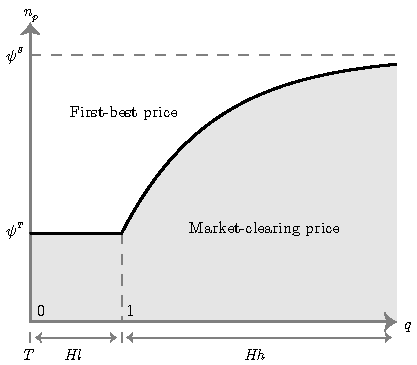
\includegraphics[scale=1.4]{old_figure/fig4_psi_v2.pdf} 
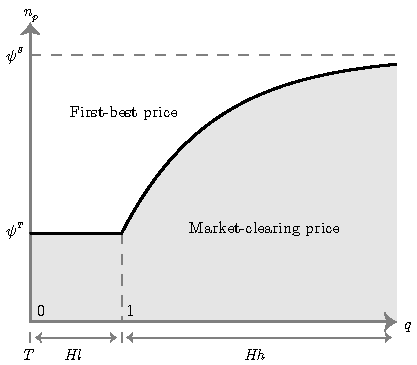
\includegraphics[width=9cm]{old_figure/fig4_psi_v2.pdf} 
\textbf{\caption{Free Bandwidth Allowance and First-best Price Thresholds\label{fig:first_best}}}
\end{figure}

For simplicity, we denote the thresholds of a two-part tariff and subscription-based pricing by $\psi^T$ and $\psi^S$, respectively. Figure \ref{fig:first_best} illustrates how the first-best price threshold $n_p$ changes with respect to the coefficient of free bandwidth allowance $q$ under hybrid pricing as shown in Lemma \ref{lem:threshold}. Specifically, when there are ample potential providers in the market compared to the threshold, the platform can achieve the highest profit using first-best prices. Otherwise, such prices do not sufficiently incentivize providers to satisfy storage demand from renters. As presented in Figure \ref{fig:first_best}, the threshold increases in $q$, suggesting that a high free bandwidth allowance discourages providers from participating in the platform due to a high operating cost involved with it. We also find that the threshold increases in $\xi \theta$, and it decreases in $\alpha$. Note that $\xi \theta$ is proportional to the total operating cost of providers, while $\alpha$ indicates the providers' revenue share. Therefore, these results indicate that the first-best prices become less feasible as providers' profitability decreases.

When the size of potential providers is insufficient to meet storage demand from renters, the platform should set market-clearing prices to incentivize providers. Specifically, for a given pricing scheme, the platform is better off increasing both $p_s$ and $p_b$ until the number of participating providers equals the number of renters willing to adopt the platform. Alternatively, the platform may incentivize providers by lowering $q$ to fulfill the storage demand from renters (Lemma \ref{lem:threshold}). In that case, since a lower free bandwidth allowance can reduce renters' utility---particularly those with high usage levels, this approach increases service costs imposed on renters.

\subsection{Optimal Redundancy Algorithm}

Recall that the P2P storage platform uses the redundancy rate denoted by $\theta$ and the uptime level $t$ to avoid security problems and ensure high capacity availability. In this subsection, we consider the platform's endogenous decision concerning the redundancy algorithm by considering its potential consequences. The redundancy algorithm may affect the behavior of renters and providers in the following ways. First, a higher redundancy rate $\theta$ indicates that each renter contracts with a larger number of providers for the same volume of files. This incurs a higher storage cost to renters and a higher storage revenue to providers, which prohibits renters from adopting the platform. In contrast, an increase in storage revenue encourages providers to join the platform. Second, the bandwidth volume transmitted through each provider decreases with $\theta$. As $\theta$ increases, more providers share the given bandwidth demand. Therefore, the bandwidth revenue and operating cost for each provider decrease. Third, a higher $\theta$ leads to a lower uptime $t$ to meet the intended availability level, lowering each provider's operating cost. Here, we derive how the platform should determine the redundancy algorithm in Theorem \ref{thm:redundancy}.

\begin{Theorem}\label{thm:redundancy}
For all pricing schemes, the profit-maximizing redundancy algorithm minimizes providers' total operating costs in the platform; that is, $\arg\max_{\theta, t} \Pi(p_s^o, p_b^o) = \arg\min_{\theta, t} \xi \theta$.
\end{Theorem}

The theorem shows that the platform always decides to set the algorithm to minimize the total operating costs of providers, which is proportional to $\xi \theta$---where $\xi$ is an increasing function of uptime $t$. A lowered operating cost implies that the P2P storage network is more efficient and attractive to potential providers, which leads to a larger number of participating providers. That is, a lower $\xi \theta$ enables the platform to serve the same number of renters with fewer potential providers and achieve first-best prices, in line with Lemma \ref{lem:threshold}.

Furthermore, we show that the optimal ($\theta$, $t$) is identical across the pricing schemes. This result is intuitive considering that lowering operating costs helps every stakeholder, and importantly, $\xi \theta$ is not a function of service fees, storage capacity, or usage levels. Based on these findings, we can directly use Lemmas \ref{lem:pricing} and \ref{lem:threshold} to compare these pricing schemes.
%
%
\section{Pricing Schemes, Profit, and System Surplus}\label{sec:analysis2}

Since the P2P storage service uses a two-sided platform with renters and providers, it often matters whether this service improves each stakeholder's surplus. As such, two-sided platforms encounter public controversies regarding whether or not they fairly reward providers \citep{gartenberg2021google, scheiber2015growth}. Moreover, consumers and politicians are concerned about the possibility that customers are unfairly treated by large platforms \citep{kosoff2015newyorkcity}. Considering that such negative sentiments might incur substantive damages to the platform \citep{cachon2017role}, it is important to understand the potential tension between the platform's profit maximization and the other stakeholders' surplus. In this regard, we analyze the impact of pricing schemes on the overall system surplus as well as the platform's profit based on the results in the previous section.

\subsection{Under First-best Prices}

As described in Section \ref{sec:analysis1}, under the given service fees ($p_s, p_b$) and total storage (paid bandwidth) volume $\upsilon_s$ ($\upsilon_{bp}$), the platform's profit $\Pi$ is:
\begin{equation*}
\Pi(p_s, p_b) = (1-\alpha) (\theta \upsilon_s p_s + \upsilon_{bp} p_b).
\end{equation*}

\noindent While providers obtain the same revenue for the storage service from renters, their operating costs differ across $\rho_j$. Thus, provider $j$ would join the platform when costs are lower than a certain threshold; that is, $\rho_j \le \rho_m$. Also, the total providers' storage volume used by the service is $V_s = \theta \upsilon_s$. Then, the provider surplus is calculated as:
\begin{equation*}
PS = \frac{\theta \upsilon_s}{\rho_m} \int_{0}^{\rho_m} \left[ \alpha \left(p_s + \frac{\upsilon_{bp}}{\theta \upsilon_s} p_b\right) - \rho \frac{\xi \upsilon_{b}}{\theta \upsilon_s}\right] d\rho.
\end{equation*}

\noindent For renter $i$, the value from service usage is $\lambda_i u_i$ and the service cost $c_i$ depends on the pricing scheme and the service fee ($p_s, p_b$). Her surplus is then calculated as $\lambda_i u_i - c_i$. As $\lambda_i$ and $u_i$ have renter-specific value whose probability distribution functions are $f(\lambda)$ and $1$ (i.e., $u_i \sim U[0, 1]$), respectively, we calculate the total surplus of renters as:
\begin{equation*}
RS = \int_{\lambda} \int_{u(\lambda)} \{\lambda u - c(\lambda, u) \}f(\lambda) du d\lambda.  
\end{equation*}

\noindent Then, we calculate the total surplus $TS$ as the sum of the platform's profit $\Pi$, provider surplus $PS$, and renter surplus $RS$ (i.e., $TS = \Pi + PS + RS$). Using the optimal service fees in each pricing scheme under the first-best prices in Lemma \ref{lem:pricing}, we obtain the platform's profit ($\Pi$) and the total surplus ($TS$) for each pricing scheme. Theorem \ref{thm:surplus_first} below shows the order of the platform's profit and the total system surplus under first-best prices:

\begin{Theorem}\label{thm:surplus_first} 
Under first-best prices, the orders of the platform's profit and the total surplus in the three pricing schemes are determined as follows:\\
\begin{table}[h] \centering
\label{tbl:thm1}
    \begin{tabular}{l  l}
        Platform's profit & $\Pi^S  \le \Pi^{Hh} \le \Pi^{Hl} = \Pi^T $\\
        %Providers' surplus & $PS^S  \le PS^{Hh} \le PS^{Hl} = PS^T $\\
        %Renters' surplus & $RS^T = RS^{Hl} \le RS^{Hh} \le RS^S$\\
        Total surplus & $TS^T = TS^{Hl} \le TS^{Hh} \le TS^S$,
    \end{tabular}
\end{table}\\
where the superscripts $T$, $Hl$, $Hh$, and $S$ indicate the two-part tariff, hybrid pricing with low $q (\le 1)$, hybrid pricing with high $q (\ge 1)$, and subscription-based pricing, respectively.
\end{Theorem}

Notably, the two-part tariff and hybrid pricing with low $q$ yield equivalent outcomes (i.e., $\Pi^{T} = \Pi^{Hl}$ and $TS^T = TS^{Hl}$). As discussed in Lemma \ref{lem:pricing}, the free bandwidth allowance is smaller than any usage level of renters when $q < 1$ (i.e., $q\lambda_0 < \lambda_0$). Therefore, the platform under hybrid pricing with low $q$ can increase $p_s$ up to the level where the platform can recover the revenue reduction from the bandwidth service without losing renters. In this way, the platform can achieve the same revenue under the two-part tariff even when they offer a limited free bandwidth allowance.

In contrast, an increase in $q$ above 1 lowers the profit of the platform (i.e., $\Pi^{Hh} \le \Pi^{Hl}$) and leads to a higher total surplus (i.e., $TS^{Hh} \ge TS^{Hl}$). The free bandwidth allowance above $\lambda_0$ enables some renters to use the entire bandwidth without the bandwidth service cost. To charge these renters, the platform would need to raise the storage service fee. Still, this does not fully recover the revenue loss from free-download volume from renters. Note that subscription-based pricing, which offers the unlimited free bandwidth allowance, can be understood as an extreme case of hybrid pricing. As $q$ increases further and goes to infinity, the platform obtains the lowest profit, and the system surplus reaches its highest value.

Remarkably, all pricing schemes attract the same number of renters to the platform under first-best prices. Therefore, differences in the total surplus are mainly driven by the difference in the usage level of renters instead of the total size of renters. Specifically, as $q$ increases, renters with a higher usage level $\lambda$---who gain a relatively high utility compared to those with a lower $\lambda$---are more likely to adopt the platform. In this way, the renters' benefit from an increase in $q$ outweighs the loss of profits, which increases the system surplus.

\subsection{Under Market-clearing Prices}

The consequences of pricing schemes under market-clearing prices are less straightforward than first-best prices because service fees can indirectly interact with renter decisions through altering the supply level. We account for this interaction and obtain the following results.

\begin{Theorem}\label{thm:surplus_market}
When the first-best price is not feasible for some pricing schemes, there exist $\underline{\psi}$ as the size of potential providers that satisfy $0  \le \underline{\psi} \le \psi^T < \psi^S$. Then, the platform's profit and total surplus in the three pricing schemes have the following orders.
\begin{enumerate}[label=(\roman*)]
    \item When $n_p$ is moderate such that $\psi^T \le n_p \le \psi^S$, a hybrid pricing with $q \ge 1$ can dominate subscription-based pricing, i.e., $\Pi^H \ge \Pi^S$ and $TS^H \ge TS^S$.
    \item When $n_p$ is small such that $\underline{\psi} \le n_p \le \psi^T $, the two-part tariff dominates subscription-based pricing; that is, $\Pi^T \ge \Pi^S$ and $TS^T \ge TS^S$.
\end{enumerate} 
\end{Theorem}

Theorem \ref{thm:surplus_market} suggests that the effectiveness of pricing schemes is highly contingent upon the number of potential providers $n_p$ in the market. When $n_p$ is large such that $n_p \ge \psi^S $, the platform can set first-best prices. Hence, all results in Theorem \ref{thm:surplus_first} hold, and subscription-based pricing---which creates the renter surplus most---always yields the highest total surplus. However, as $n_p$ decreases, first-best prices become insufficient to incentivize providers. Hence, the platform should give a higher reward to each provider to maintain the same level of capacity. This result indicates that the size of potential providers needs to be carefully considered in the platform's pricing decisions. 

We further investigate how optimal service fees in the pricing schemes interplay with $n_p$ and find the following results. First, as $n_p$ is moderate such that $\psi^T \le n_p \le \psi^S$, there exists some hybrid pricing with $q \ge 1$ that outweighs the subscription-based pricing in terms of total surplus as well as the platform's profit. As suggested by Lemma \ref{lem:threshold}, first-best prices are not applicable for subscription-based pricing when $n_p$ is moderate. Hence, the profit-seeking platform needs to adopt market-clearing prices to incentivize providers and avoid rationing renters who are willing to pay for the service. Thus, subscription-based pricing experiences a significant decline in the platform's profit, provider surplus, and renter surplus. Alternatively, the platform may achieve first-best prices by reducing the free bandwidth allowance. By balancing the incentive for providers and the renters' utility from the free bandwidth allowance, the platform can achieve a higher total surplus when the number of potential providers is comparable to the number of potential renters.

Second, we show that the two-part tariff dominates subscription-based pricing in terms of the platform's profit and total surplus when $n_p$ is small such that $\underline{\psi} \le n_p \le \psi^T $. In this case, the platform should attract a large proportion of potential providers to meet the same storage demand from renters. Then, the free bandwidth allowance affects the platform's ability to fulfill the storage demand more adversely. The platform needs to set strikingly high subscription fees to compensate for this adverse effect, and consequently, the renter surplus---the main advantage of subscription-based pricing---decreases substantially. In contrast, a two-part tariff can maintain the required capacity for market-clearing with relatively cheap service fees because it rewards providers for all bandwidth provision. As a consequence, a two-part tariff can achieve a higher system surplus than subscription-based pricing, implying that rewarding providers could be more beneficial to the entire system than focusing on the renter surplus.
%
%
\section{Model Extension and Discussion}\label{sec:analysis3}

\subsection{\textcolor{blue}{Assumptions on the Platform}}
% Endogenous Decision on Commission Rates

\textcolor{blue}{Thus far, we have assumed an exogenously given commission rate when investigating the platform's optimal service fees. It is difficult for two-sided platforms to alter commissions as they often encounter public controversies regarding whether or not they fairly reward providers \citep{gartenberg2021google, scheiber2015growth}. However, it is still informative to understand how the implications of pricing schemes change when the platform is free to adjust its commission rate. Therefore, in this subsection, we consider an endogenously determined commission rate for the platform. Now,} the platform can choose a commission rate to better maximize its profit. Also, it is possible that such a benefit may be amplified under a non-flexible pricing scheme (e.g., subscription-based pricing). To verify the possibility that the endogenous selection of commission rates affects our findings, we re-analyze our model by considering $\alpha$ as a decision variable as well as $p_s$ and $p_b$. Theorem \ref{thm:alpha} summarizes the results \textcolor{blue}{according to the exogenous size of potential providers $n_p$}. 

\begin{Theorem}\label{thm:alpha}
If the profit-seeking platform endogenously determines the commission rate, there exists $\bar{\psi}_{\alpha}$ as the size of potential providers that satisfies $0 \le \psi_{\alpha}^T \le \bar{\psi}_{\alpha} \le \psi_{\alpha}^S$, where $\psi_{\alpha}^T \equiv \frac{1}{2}\xi \theta n_r$ and $\psi_{\alpha}^S \equiv 3 \xi \theta n_r$. Then, the platform's profit and the total surplus in the three pricing schemes have the following orders.
\begin{enumerate}[label=(\roman*)]
    \item When $n_p$ is large such that $n_p \ge \bar{\psi}_{\alpha}$, the two-part tariff generates the highest platform's profit, while subscription-based pricing yields the highest total surplus (Theorem \ref{thm:surplus_first}).
    \item When $n_p$ is moderate such that  
    $\psi_{\alpha}^T \le n_p \le \bar{\psi}_{\alpha}$, a hybrid pricing with some $q \ge 1$ dominates subscription-based pricing. That is, $\Pi^H \ge \Pi^S$ and $TS^H \ge TS^S$ (Theorem \ref{thm:surplus_market} (\textit{i})),
    \item When $n_p$ is small such that $0 \le n_p \le \psi_{\alpha}^T$, the two-part tariff dominates subscription-based pricing. That is, $\Pi^T \ge \Pi^S$ and $TS^T \ge TS^S$ (Theorem \ref{thm:surplus_market} (\textit{ii})).
\end{enumerate}
\end{Theorem}

\textcolor{blue}{The theorem shows that our main insights obtained in Theorems \ref{thm:surplus_first} and \ref{thm:surplus_market} continue to hold, although the thresholds for first-best prices change. %Specifically, we observe that the relative orders of pricing schemes by the platform's profit and the total surplus do not change by the endogeneity of the commission rate. 
This suggests that it is still crucial for the platform to incentivize providers, even when it is free to alter its commission rate to increase its own profit.}

Although the results from endogenous commission rates are consistent with our main findings, we should interpret them with caution for the following reasons. First, two-sided platforms need to carefully consider public sentiment as well as profits because they often encounter public controversies regarding whether they fairly reward providers \citep{gartenberg2021google, scheiber2015growth}. Second, potential competition and regulations might inhibit platforms from choosing high commission rates for providers. Even when competitors are not strong or even absent, unsatisfactory rewards for storage supply might encourage new entrants to grow their shares in the market. Lastly, the suggested commission rates might be unrealistic. Sia's commission rate is about 3.9\%, and mobile app stores---i.e., Google Play and Apple's App Store---charge 30\% to app providers. Considering the fierce resistance to 30\% commission rates in app markets \citep{gartenberg2021google}, 67\% or higher commission rates might not be a viable option.\footnote{Please refer to the proof in Online Appendix \ref{app:proof} for magnitudes of commission rates.} For these reasons, the assumption of exogenous commission rates can be reasonably acceptable in our context.

% \subsection{Discussion on Assumptions}

\subsection{\textcolor{blue}{Assumptions on Providers}}

% R1's Point 1 (Redundancy's feasibility)
%We have made several assumptions about providers and renters, which might have driven our findings. 
In this subsection, we discuss the plausibility and potential consequences of assumptions on providers, and if applicable, conduct numerical analyses to quantitatively examine these issues. Specifically, our model excludes cases wherein operating costs are negligible for potential providers; that is, we assume that $\xi > \frac{3}{4} \alpha$. Although online forums for P2P storage platforms have been significantly concerned with profitability and operating costs, it is still important to understand the consequences of pricing schemes when operating costs become negligible. In Online Appendix C, we provide technical details of a numerical study examining how small operating costs (i.e., $\xi \le \frac{3}{4} \alpha$) can affect our results. Below, we summarize key insights from this analysis.

When $\xi$ is substantially small (i.e., low operating costs), all potential providers are willing to share their storage and participate in the platform. Since providers do not respond to bandwidth fees sensitively under small $\xi$, raising prices does not help renters find more capacity but does increase their financial burden. Therefore, a two-part tariff and hybrid pricing, which compensate for providers' bandwidth services, are less effective in boosting system surplus than subscription-based pricing. Consequently, the surplus implication of pricing schemes is similar to first-best prices under substantially small $\xi$.

% R2's Point A2b (Proportional operating costs/storage volume heterogeneity)
Second, one might consider an alternative form of the provider's operating cost. Basically, the current form relies on the assumptions that operating costs are proportional to $\hat{\omega_b}$ (i.e., expected bandwidth volume for each provider), and that $\hat{\omega_b}$ is proportional to each provider's shared storage capacity. We argue that these assumptions are plausible for the following reasons: 1) many of the major costs, such as Internet bandwidth and electricity costs, are proportional to bandwidth usage, and 2) the platform tends to assign more files and bandwidth services to high-capacity providers than low-capacity ones.

So, how would alternative cost forms affect the results? On the one hand, we may consider a convex function, such as quadratic and exponential forms, wherein operating costs are particularly burdensome for high-capacity providers. In this case, as high-capacity providers bear much higher operating costs and join the platform less, compensating for offering bandwidth services will have a higher impact on storage capacity. Consequently, the relative benefits of a two-part tariff and hybrid pricing (vs. subscription-based pricing) will be greater in this situation. On the other hand, we may also consider a concave function like a square root function. Since high-capacity providers bear relatively less operating burden than they do in the current setup, the platform will attract more providers under subscription-based pricing. Hence, the profit/surplus gap between subscription and other pricing schemes will decrease as a result. However, although the magnitudes decline, we expect the differences to remain qualitatively unchanged.

% R2's Point A3 (Informed decision)
Third, and importantly, one might wonder if providers can meaningfully predict demand for storage and bandwidth services in advance. We argue that providers can make informed choices based on multiple sources that offer information before joining the platform. For example, individual providers have actively analyzed and shared their profitability in online forums, such as Reddit. Also, P2P storage platforms notice the minimum requirements and recommended capacity of computing resources before individuals decide to join their networks. Such information can partially inform them about expected operational costs. They also publicize their storage sharing status, such as used storage, number of transactions, network revenues, and hash rates (e.g., SiaStats). Moreover, even when unsuccessful on the platform, they can quickly leave the network, similar to other digital markets. In sum, due to the platform-offered information, online forums, and easiness of market entry/exit, we expect that participants in the platform will rapidly reach market equilibrium.

\subsection{\textcolor{blue}{Assumptions on Renters}}

\textcolor{blue}{In this subsection, we investigate the potential consequences of  assumptions on renters.  Specifically, we conduct numerical analyses on our assumptions on renter heterogeneity. We report the technical details in Online Appendix C.} 

\textcolor{blue}{We find the following main insights. First, our numerical experiments suggest that our findings remain consistent when we relax the assumption of bandwidth usage distribution of renters. \footnote{\textcolor{blue}{For this result, we assume that bandwidth usage follows the Pareto distribution with $b=2$ to account for the heavy-tail distribution and analytical tractability. To assess whether this assumption is entirely responsible for our findings, we conduct a numerical analysis of different shapes of distributional tails. For ease of comparison, we have varied the Pareto’s shape parameters and tested whether our findings continue to hold.}} The results indicate that the implications of pricing schemes do not change under different parametric conditions.} 

% R2's Points A4a (Renter's independence between utility per download and download frequency)

\textcolor{blue}{Second,} our model postulates that the distributions of the utility per bandwidth volume and the download frequency are independent. Although this leads to a positive association between these variables as a result of self-selection, it is also possible that they are positively associated with each other before the renter's decision. %We examine whether the implications of pricing schemes are qualitatively consistent after relaxing this assumption by conducting a numerical study. 
We observe that our main findings remain qualitatively consistent.

% R2's Points A2a (Renter's storage volume heterogeneity)
Lastly, we further consider an additional dimension of heterogeneity: storage demand. One may be concerned that our assumption of homogeneous storage demand may have driven our findings. In particular, pricing schemes might have unexpected influences if their storage and bandwidth needs are correlated. \textcolor{blue}{To assess this possibility, we conduct numerical analyses utilizing various distributions of storage and bandwidth volumes. We observe that the main insights from the basic setup remain qualitatively unchanged in our results \footnote{\textcolor{blue}{However, when we allow some renters to have more storage demand than unit volume, a larger share of renters may need more bandwidth capacity than the bandwidth allowance. Consequently, the influence of hybrid pricing becomes similar to that of a two-part tariff, altering the boundaries in Theorem \ref{thm:surplus_market}.}} %Except for this, we do not see any changes from relaxing the assumption.
}
%
\section{Conclusions}

% Research summary
In this study, we developed a game-theoretic model to examine how the P2P storage platform's pricing schemes impact the platform's profit and the total system surplus. We considered three pricing schemes, one of which is widely employed by P2P storage platforms (two-part tariffs) while the others are widely adopted by conventional public cloud services (subscription-based pricing and the hybrid pricing). Also, we incorporated endogenous decisions on redundancy algorithms into deciding profit-maximizing service fees under a given pricing scheme.

We showed that when first-best prices---which maximize the platform's profit when the number of potential providers is sufficient---are applicable, the two-part tariff outperforms other pricing schemes in terms of profit maximization, while subscription-based pricing surpasses the others regarding total surplus. Remarkably, we revealed that the relative influences of pricing schemes significantly change when the scarcity of potential providers is considered. When potential providers are not sufficient to meet storage demand, the platform cannot set first-best prices. Instead, it should employ the market-clearing prices wherein supply and demand become equivalent. In this case, the two-part tariff and hybrid pricing may dominate subscription-based pricing regarding both profit and total surplus. To further validate our findings, we examined how endogenous commission rates and relaxing other assumptions affect the results. We found that our key findings remain qualitatively unchanged.

% Managerial implications for P2P storage platforms
Our findings provide numerous implications for P2P storage platforms that rely on independent suppliers and concern the surplus of stakeholders. We compared the currently adopted pricing scheme with other pricing schemes rarely used by P2P storage platforms and revealed that the scarcity of potential providers plays a central role in determining the effects of pricing schemes. Specifically, we showed that if there is a sufficiently large base of potential suppliers, the platform can enhance the total surplus of the system by adopting subscription-based pricing instead of a two-part tariff. On the other hand, if the size of potential providers is not sufficient, subscription-based pricing might lead to a lower surplus than a two-part tariff and hybrid pricing, which will ensure a higher profit for the platform. In addition, our results suggest that the effectiveness of a pricing scheme substantially interplays with the redundancy algorithm. Specifically, the two-part tariff and the hybrid pricing become increasingly effective as the redundancy algorithm requires a higher uptime and redundancy rate, raising providers' operating costs.

In this vein, our findings provide actionable insights that these platforms can directly apply. Given the immature stage of the P2P storage market, platforms might want to expand their user base by increasing the total system surplus rather than seeking short-term profit only. In doing so, they may consider adopting alternative pricing schemes that can yield a higher surplus than a two-part tariff. However, it could be difficult to attract potential providers to the platform, due to technical difficulties of sharing computing resources. If so, the P2P storage platform needs to further compensate providers' bandwidth provision rather than their storage capacity by lowering the free bandwidth allowance. It is also possible that the platform cannot alter its pricing scheme and service fees. In that case, the platform may indirectly incentivize providers by requiring a lower uptime or a lower redundancy rate. For instance, a $k$-of-$m$ erasure coding scheme with the same redundancy rate (i.e., the same $\frac{m}{k}$) can achieve the same availability while reducing its required uptime by increasing $k$ and $m$ at the same time.\footnote{Table \ref{tbl:redundancy_1} in Online Appendix \ref{app:algorithm} shows an example suggesting that the platform can exponentially reduce failure probability while maintaining the redundancy rate.}

% Managerial implications for other types of platforms
Our research also provides managerial insights that other sharing platforms can also consider. We found that pricing schemes that further compensate providers can improve the total surplus when the size of potential suppliers is relatively smaller than that of consumers. Although other platforms often employ different pricing schemes, the underlying intuition could be similarly applied to these platforms. We showed that a rise in service prices could mitigate this situation in which only a few providers endure high operating costs. In this regard, sharing platforms may consider heterogeneous pricing strategies across regions. For example, peer-to-peer delivery platforms serve various regions with different sizes of sellers, deliverers, and consumers. In regions where relatively few deliverers are bearing delivery costs, platforms may achieve not only higher profits but also a higher surplus of all stakeholders by further charging sellers/consumers. In contrast, the system surplus will be increased by lowering service prices when sufficient deliverers are in the regions.

%(P5) Limitation and future research
We conclude by specifying some caveats and potential avenues for future research. First, we have analyzed only a monopoly market. The P2P storage market is highly immature and still rapidly growing, and several new entrants are threatening incumbent players. We expect that future research can significantly benefit from investigating the influence of competitors in this nascent market. Second, our model relies on homogeneous storage volume in order to focus on interactions between renters and providers. Although the numerical analysis suggests that our findings are insensitive to renter's heterogeneous storage, future studies can make substantial progress by incorporating the heterogeneity of storage volume from the supply and demand sides into their main models. Lastly, our results are restricted to three pricing schemes, but many other pricing schemes can be considered. For instance, some public cloud services lower the unit price as the usage level increases. Analyzing how unexplored pricing schemes affect the platform's profit and system surplus can provide valuable insights. 
%
%
%	\bibliographystyle{informs2014}
	%\bibliographystyle{apacite}
	\bibliographystyle{pomsref}
	\bibliography{bib}
%
%
\newpage	
\noindent \textbf{\LARGE Online Appendices}
\appendix
\section{Algorithmic Backgrounds}\label{app:algorithm}
In general, P2P storage platforms utilize erasure coding in their redundancy algorithms to ensure high levels of file availability. Under a $k$-of-$m$ erasure coding scheme, the P2P storage platform divides a renter's original file into $k$ shards and re-codes them into $m$ encrypted fragments ($m > k$) \citep{weatherspoon2002erasure, wilkinson2016storj}. Then, the platform assigns each of $m$ fragments to $m$ independent providers who have made a contract with the focal renter. Notably, any $k$ of $m$ fragments can reconstruct the file under this redundancy algorithm. Therefore, the platform can retrieve the file when any $k$ providers are connected to the network at the same time. As such, the main advantage of erasure coding is that it can achieve high reliability with a low redundancy rate $\theta(=\frac{m}{k})$ \citep{weatherspoon2002erasure}. We can easily estimate the reliability of the P2P storage networks as follows. Given the redundancy parameters $k$, $n$ and the required uptime $t$, the failure probability is calculated as:

\begin{equation*}
\begin{aligned}
F(t; m, k) = \sum_{j=0}^{k-1} {m \choose j}t^j (1-t)^{m-j}
\end{aligned}
\end{equation*}

From the equation above, we obtain the following relationships between the failure probability, the redundancy parameters and the required uptime:

\begin{Lemma}\label{lem:uptime}
i) $F(t; m, k)$ is decreasing in $t$ for fixed $m$ and $k$,\\
ii) $F(t; m, k)$ is decreasing in $m$ for fixed $t$ and $k$.
\end{Lemma}

Lemma \ref{lem:uptime} provides insight into how each parameter affects the failure probability. First, the failure probability decreases when the platform requires a higher uptime to the provider, indicating that the platform can enhance the reliability while maintaining the same redundancy rate by imposing higher responsibility on the provider. Second, if the platform assigns the file fragments to a larger number of providers, the failure probability decreases. It suggests that the platform can improve the file availability by increasing the number of providers instead of imposing higher responsibility on each provider.

Table \ref{tbl:redundancy_1} presents the calculated failure probability under the given redundancy $\theta = 3$. We observe that the platform can improve its system reliability even when it maintains the same redundancy $\theta$ and the same required uptime $t$. For instance, for $\theta=3$ and $t=0.75$, the failure probability is 1.15e-04 when the platform sets $k=5$ and $m=15$. Notably, the platform can reduce the failure probability by about 400 times (from 1.15e-04 to 2.82e-07) by dividing the files into twice more fragments ($k=10$ and $m=30$) without altering $\theta$ and $t$. Moreover, we see that a small increase in the required uptime can dramatically reduce the failure probability. For example, when all other things are same, raising the required $t$ by 20\% (from 0.75 to 0.90) under $k=10$ and $n=30$ decreases the failure by 48.6 million times (from 2.82e-07 to 5.80e-15).

\begin{table}[h]
\textbf{\caption{An Example of Redundancy Algorithm and Failure Probability ($\theta=3$)\label{tbl:redundancy_1}}}
\begin{center}
\begin{tabular}{cccc}
 $m$ & $k$ & $t$ & $F(t; m, k)$\\\hline
15 & 5 & 0.5 & 5.92e-02\\
15 & 5 & 0.75 & 1.15e-04\\
15 & 5 & 0.9 & 9.30e-09\\
15 & 5 & 0.99 & 1.32e-19\\
30 & 10 & 0.5 & 2.14e-02\\
30 & 10 & 0.75 & 2.82e-07\\
30 & 10 & 0.9 & 5.80e-15\\
30 & 10 & 0.99 & 1.31e-35\\
\end{tabular}
\end{center}
\end{table}

In addition to erasure coding, P2P storage platforms are taking several measures to prevent the strikingly adverse effect of file transfer failure. For instance, P2P storage platforms usually require providers to meet the minimum available storage space, computing power of processors, and bandwidth speed. Also, they mandate the uptime level in various ways. Sia expects providers to maintain 95–98\% uptime to achieve 99.9999\% accessibility of stored files. If a provider in the Sia network does not maintain 95\% uptime (or 36 hours off in a month), he will lose his collateral for active contracts. Storj requires a more demanding uptime requirement that requires providers to maintain 99.3\% uptime (or 5 hours of maximum downtime per month). Filecoin assesses miners in the cryptocurrency network and penalizes storage providers using the miners' collateral if they do not perform the proof-of-spacetime. Hypothetically, Sia and Storj are expected to achieve the very low failure probability as 2.52e-29 and 2.11e-91 based on their algorithm parameters ($k, m, t$) as $(10, 30, 0.98)$ and $(29, 80, 0.993)$, respectively.\footnote{The relevant information was retrieved from the following sources: 1) Storj's redundancy parameters (https://docs.storj.io/concepts/overview), 2) Storj's required uptime (https://www.storj.io/node-operator-terms-conditions), 3) Sia's redundancy parameters (https://support.sia.tech/renting/is-my-data-secure\#security), 4) Sia's required uptime (https://support.sia.tech/hosting/about-hosting-on-sia).} According to Storj, the Tardigrade platform---Storj's main service---demonstrated 99.96\% availability in practice.\footnote{Please refer to the following webpage for further details: https://www.storj.io/blog/announcing-pioneer-2-and-tardigrade-io-pricing.}

If we assume that the target failure probability $\bar{p}$ is close to zero, i.e., $\bar{p} \approx 0$, the platform's redundancy parameters and the required uptime satisfy the following equation:
\begin{equation*}
\begin{aligned}
F(t; m, k) = \sum_{j=0}^{k-1} {m \choose j}t^j (1-t)^{m-j} \le \bar{p}.
\end{aligned}
\end{equation*}
As shown in Lemma \ref{lem:uptime}, the platform achieves its target failure probability by requiring a high uptime $t$ or adopting a high redundancy rate $\theta$. Table \ref{tbl:redundancy_2} presents the calculated pair of the redundancy rate and the required uptime for $k=10$ and the target probability $\bar{p} = 10e-10$. Figure \ref{fig:redundancy} visualizes this relationship. When a redundancy rate is low, increasing $\theta$ does not significantly decrease the required uptime. For instance, when $\theta$ increases from 1 to 1.5, the required $t$ decreases by only 0.005. In contrast, when we compare $\theta = 3$ and $\theta = 3.5$, the required uptime decreased by (from 0.836 to 0.776).

\begin{table}[h]
\textbf{\caption{An Example of Redundancy Rate and Uptime ($k=10$, $\bar{p} = 10^{-10}$)\label{tbl:redundancy_2}}}
\begin{center}
\begin{tabular}{cccccc}
 $\theta$ &$t$&$\theta$ & $t$&$\theta$&$t$\\\hline
$\le$1.2 & 1 & 2.0 & 0.957 & 2.8 & 0.861\\
1.3 & 0.999 & 2.1 & 0.947 & 2.9 & 0.849\\
1.4 & 0.998 & 2.2 & 0.935 & 3.0 & 0.836\\
1.5 & 0.995 & 2.3 & 0.924 & 3.1 & 0.824\\
1.6 & 0.990 & 2.4 & 0.911 & 3.2 & 0.812\\
1.7 & 0.984 & 2.5 & 0.899 & 3.3 & 0.800\\
1.8 & 0.976 & 2.6 & 0.886 & 3.4 & 0.788\\
1.9 & 0.967 & 2.7 & 0.874 & 3.5 & 0.776\\
\end{tabular}
\end{center}
\end{table}

\begin{figure}[ht!]
\centering
\includegraphics[width=10cm]{figure_3rd_final/uptime_fig.jpg} 
\textbf{\caption{Redundancy Rate and Required Uptime ($k=10$, $\bar{p} = 10^{-10}$)\label{fig:redundancy}}}
\end{figure}


\newpage
\section{Proof}\label{app:proof}
% Before we proceed the proofs of the main results, we analyze providers' participation decision to the P2P storage service and derive the results in the lemma below.

\paragraph{Proof of Lemma \ref{lem:pvd_chr}}
\begin{proof}
Provider \textit{j}'s cost increases in $\rho_j$. Thus, if $\pi|_{\rho_j = 1} \ge 0$, all providers are profitable (i.e., $\rho_m = 1$). Otherwise, if $\pi|_{\rho_j= 1} <0$, there exists $\rho_m < 1$ that satisfies $\pi|_{\rho_j = \rho_m} = 0$. Also, if $\omega_s \le \theta \upsilon_s $, all providers' utilization becomes $1$. In contrast, when $\theta \upsilon_s < \omega_s $, all providers' utilization is strictly lower than $1$. We thus consider the following cases:
\begin{table}[h]
\begin{center}
\begin{tabular}{c|cc}
&$\pi|_{\rho_j = 1} \ge 0$ & $\pi|_{\rho_j = 1} < 0$\\\hline 
$\omega_s \le \theta \upsilon_s$ & $\rho_m = 1$, $\hat{\omega}_s=1 $ & $\rho_m < 1$, $\hat{\omega}_s=1 $\\
$\theta \upsilon_s < \omega_s$& $\rho_m = 1$, $\hat{\omega}_s<1 $ & $\rho_m < 1$, $\hat{\omega}_s<1 $\\
\end{tabular}
\end{center}
\end{table}

\noindent \textbf{A. Analysis of Cases and Sub-conditions}\\
We analyze the four cases as follows. First, we derive the outcome of each case and its sub-conditions. Then, we assess the feasibility of these outcomes.\\

\noindent \textbf{\textit{Case A1:}} $\pi|_{\rho_j =1} \ge 0$ and $\omega_s \le \theta \upsilon_s$.

\noindent This condition leads to $\rho_m = 1$ and $\hat{\omega}_s = 1$. For each of the two sub-conditions, we obtain the followings:

\textit{\underline{Sub-condition A1-i:}} $\pi|_{\rho_j = 1} \ge 0$:
\begin{equation*}
\begin{aligned}
&\pi|_{\rho_j = 1} \ge 0 \Leftrightarrow \alpha p_s + \alpha p_b \frac{\upsilon_{bp}}{\theta \upsilon_s} - \frac{\xi \upsilon_b}{\theta \upsilon_s} \ge 0 \\
&\Leftrightarrow \frac{\xi \upsilon_b}{\theta \upsilon_s} \le \alpha p_s + \alpha p_b \frac{\upsilon_{bp}}{\theta \upsilon_s} \Leftrightarrow g_1 \le \tilde{\pi}, 
\end{aligned}
\end{equation*}

\textit{\underline{Sub-condition A1-ii:}} $\omega_s \le \theta \upsilon_s$:
\begin{equation*}
\begin{aligned}
&\omega_s \le \theta \upsilon_s \Leftrightarrow n_p \le \theta \upsilon_s.
\end{aligned}
\end{equation*}

As a result, we obtain $(\rho_m, \hat{\omega}_s) = (1, 1)$.\\

\noindent \textbf{\textit{Case A2:}} $\pi|_{\rho_j =1} <0$ and $\omega_s \le \theta \upsilon_s$.\\
\noindent In this condition, $\rho_m <1$ and $\hat{\omega}_s = 1$. Then, the sub-conditions lead to the following results:

\textit{\underline{Sub-condition A2-i:}} $\pi|_{\rho_j = \rho_m} = 0$ where $\rho_m < 1$: 
\begin{equation*}
\begin{aligned}
&\pi|_{\rho_j = \rho_m} = 0 \Leftrightarrow \alpha p_s + \alpha p_b \frac{\upsilon_{bp}}{\theta \upsilon_s} - \rho_m \frac{\xi \upsilon_b}{\theta \upsilon_s} = 0 \Leftrightarrow \rho_m = \frac{\alpha p_s + \alpha p_b \frac{\upsilon_{bp}}{\theta \upsilon_s}}{\frac{\xi \upsilon_b}{\theta \upsilon_s}} \\
&\Rightarrow \rho_m < 1 \Leftrightarrow \frac{\alpha p_s + \alpha p_b \frac{\upsilon_{bp}}{\theta \upsilon_s}}{\frac{\xi \upsilon_b}{\theta \upsilon_s}} < 1 \Leftrightarrow \tilde{\pi}<g_1,
\end{aligned}
\end{equation*} 

\textit{\underline{Sub-condition A2-ii:}} $\omega_s \le \theta \upsilon_s$:
\begin{equation*}
\begin{aligned}
&\omega_s \le \theta \upsilon_s \Leftrightarrow n_p \rho_m \le \theta \upsilon_s \Leftrightarrow n_p \frac{\alpha p_s + \alpha p_b \frac{\upsilon_{bp}}{\theta \upsilon_s}}{\frac{\xi \upsilon_b}{\theta \upsilon_s}} \le \theta \upsilon_s\\
&\Leftrightarrow \alpha p_s + \alpha p_b \frac{\upsilon_{bp}}{\theta \upsilon_s}  \le \frac{\xi \upsilon_b}{n_p} \Leftrightarrow \tilde{\pi} \le g_2. 
\end{aligned}
\end{equation*}

It follows that $(\rho_m, \hat{\omega}_s) = (\frac{\tilde{\pi}}{g_1}, 1)$.\\

\noindent \textbf{\textit{Case A3:}} $\pi|_{\rho_j =1} \ge 0$ and $\theta \upsilon_s < \omega_s $.\\
This condition results in $\rho_m = 1$ and $\hat{\omega}_s = \frac{\theta \upsilon_s}{\omega_s}$. The two sub-conditions lead to the followings:

\textit{\underline{Sub-condition A3-i:}} $\pi|_{\rho_j = 1} \ge 0$:
\begin{equation*}
\begin{aligned}
&0 \le \pi|_{\rho_j = 1} \Leftrightarrow 0 \le \alpha p_s + \alpha p_b \frac{\upsilon_{bp}}{\theta \upsilon_s} - \frac{\xi \upsilon_b}{\theta \upsilon_s}\\
&\Leftrightarrow \frac{\xi \upsilon_b}{\theta \upsilon_s} \le \alpha p_s + \alpha p_b \frac{\upsilon_{bp}}{\theta \upsilon_s} \Leftrightarrow g_1 \le \tilde{\pi}, 
\end{aligned}
\end{equation*}

\textit{\underline{Sub-condition A3-ii:}} $ \theta \upsilon_s < \omega_s$:
\begin{equation*}
\begin{aligned}
&\theta \upsilon_s < \omega_s \Leftrightarrow \theta \upsilon_s < n_p.
\end{aligned}
\end{equation*}

Then, $ (\rho_m, \hat{\omega}_s) = (1, \frac{\theta \upsilon_s}{n_p})$.\\

\noindent \textbf{\textit{Case A4:}} $\pi|_{\rho_j =1} <0$ and $\theta \upsilon_s < \omega_s $.\\
This condition leads to $\rho_m <1$ and $\hat{\omega}_s = \frac{\theta \upsilon_s}{\omega_s}$. For the two sub-conditions, we obtain the followings:

\textit{\underline{Sub-condition A4-i:}} $\pi|_{\rho_j = \rho_m} = 0$ where $\rho_m < 1$:
\begin{equation*}
\begin{aligned}
&\pi|_{\rho_j = \rho_m} = 0 \Leftrightarrow \alpha p_s + \alpha p_b \frac{\upsilon_{bp}}{\theta \upsilon_s} - \rho_m \frac{\xi \upsilon_b}{\theta \upsilon_s} = 0 \Leftrightarrow \rho_m = \frac{\alpha p_s + \alpha p_b \frac{\upsilon_{bp}}{\theta \upsilon_s}}{\frac{\xi \upsilon_b}{\theta \upsilon_s}} \\
&\Rightarrow \rho_m < 1 \Leftrightarrow \frac{\alpha p_s + \alpha p_b \frac{\upsilon_{bp}}{\theta \upsilon_s}}{\frac{\xi \upsilon_b}{\theta \upsilon_s}} < 1 \Leftrightarrow \tilde{\pi} < g_1,
\end{aligned}
\end{equation*}

\textit{\underline{Sub-condition A4-ii:}} $\theta \upsilon_s < \omega_s$: 
\begin{equation*}
\begin{aligned}
&\theta \upsilon_s < \omega_s \Leftrightarrow \theta \upsilon_s < n_p \rho_m \Leftrightarrow \theta \upsilon_s < n_p \frac{\alpha p_s + \alpha p_b \frac{\upsilon_{bp}}{\theta \upsilon_s}}{\frac{\xi \upsilon_b}{\theta \upsilon_s}} \\
&\Leftrightarrow   \frac{\xi \upsilon_b}{n_p}  <   \alpha p_s + \alpha p_b \frac{\upsilon_{bp}}{\theta \upsilon_s} \Leftrightarrow g_2 < \tilde{\pi}.   
\end{aligned}
\end{equation*}

Therefore, we observe that $ (\rho_m, \hat{\omega}_s) = (\frac{\tilde{\pi}}{g_1}, \frac{g_2}{\tilde{\pi}} )$. \\

\noindent \textbf{B. Feasibility Analysis}\\
For the results obtained above, we analyze the feasibility of each case. Since $\theta \upsilon \lessgtr n_p \Leftrightarrow g_2 \lessgtr g_1$ holds, we consider the following cases:\\

\noindent \textbf{\textit{Case B1:}} $\theta \upsilon_s \le n_p$.\\
This case implies $g_2 \le g_1$. By using this property, we analyze the feasible region for each of the cases in part A:

\textbf{\textit{Case A1:}} infeasible,

\textbf{\textit{Case A2:}} when $\tilde{\pi} \le g_2$, $(\rho_m, \hat{\omega}_s) = (\frac{\tilde{\pi}}{g_1}, 1)$,

\textbf{\textit{Case A3:}} when $g_1 \le \tilde{\pi}$, $(\rho_m, \hat{\omega}_s) = (1, \frac{\theta \upsilon_s}{n_p})$,

\textbf{\textit{Case A4:}} when $g_2 < \tilde{\pi} < g_1$, $(\rho_m, \hat{\omega}_s) = (\frac{\tilde{\pi}}{g_1}, \frac{g_2}{\tilde{\pi}})$.

Combining these feasible regions and the continuity of $(\rho_m, \hat{\omega}_s)$ across the cases, we obtain the results for $\theta \upsilon_s \le n_p$, as shown in Lemma \ref{lem:pvd_chr}.\\

\noindent \textbf{\textit{Case B2:}} $\theta \upsilon_s \ge n_p$.
In this case, we see $g_2 \ge g_1$. For each case in the part A, we obtain the feasible region as follows:

\textbf{\textit{Case A1:}} when $g_1 \le \tilde{\pi}$, $(\rho_m, \hat{\omega}_s) = (1, 1)$,

\textbf{\textit{Case A2:}} when $\tilde{\pi} < g_1$, $(\rho_m, \hat{\omega}_s) = (\frac{\tilde{\pi}}{g_1}, 1)$,

\textbf{\textit{Case A3:}} infeasible,

\textbf{\textit{Case A4:}} infeasible.

Incorporating these feasible regions and the continuity of $(\rho_m, \hat{\omega}_s)$, we obtain the results for $n_p \le \theta \upsilon_s$ in Lemma \ref{lem:pvd_chr}.
\end{proof}


\paragraph{Proof of Lemma \ref{lem:pricing}}
\begin{proof}
We derive the profit-maximizing service fees for each pricing scheme. In doing so, we separate the hybrid pricing into two cases based on whether the free bandwidth allowance exceeds the minimum usage level $\lambda_0$.\\  

\noindent \textbf{\textit{Case 1: The Two-part Tariff.}}\\
We consider the two sub-cases according to the value of the storage service fee $p_s$ as follows:

\textit{\underline{Sub-case 1-i:}} $0 \le p_s \le \frac{\lambda_0 - \lambda_0 p_b}{\theta}$.

Regarding renters willing to adopt the platform, the total storage volume $\upsilon_s$ and the total paid bandwidth volume $\upsilon_{bp}$ are derived as follows:
\begin{equation*}
\begin{aligned}
&\upsilon_s = n_r \int_{\lambda_0}^{\infty}(1-\frac{\theta p_s}{\lambda} - p_b) f(\lambda) d \lambda = n_r(1-\frac{2\theta p_s}{3\lambda_0} - p_b),\\
&\upsilon_{bp} = n_r \int_{\lambda_0}^{\infty}\lambda (1-\frac{\theta p_s}{\lambda} - p_b) f(\lambda) d \lambda  = n_r\left[-\theta p_s + 2\lambda_0 (1-p_b) \right].
\end{aligned}
\end{equation*}

Using the derived $\theta \upsilon_s$ and $\upsilon_{bp}$, we can rewrite the platform's objective function as:
\begin{equation*}
\max_{p_s, p_b}\Pi(p_s, p_b) = (1-\alpha) \theta n_r \left( - \frac{2\theta}{3\lambda_0} p_s^2 - 2 p_s p_b - \frac{2\lambda_0}{\theta} p_b^2 + p_s + \frac{2\lambda_0}{\theta} p_b\right).
\end{equation*}

We verify the second-order condition by analyzing the Hessian matrix of that profit function
\begin{equation*}
H=\begin{bmatrix}
-\frac{4(1-\alpha) \theta^2 n_r}{3\lambda_0} & -2(1-\alpha) \theta n_r\\
-2(1-\alpha) \theta n_r & -4 (1-\alpha) \lambda_0 n_r
\end{bmatrix}.
\end{equation*}

We observe that the first-order leading principal minor is negative and the second-order leading principal minor is $det(H) = \frac{4}{3}(1-\alpha)^2 \theta^2 n_r^2 >0$. Therefore, $H$ is negative-definite. Hence, the second-order condition is satisfied, and this profit function has the global maximum. Based on these results, we obtain the optimal service fees as:\\
\begin{equation*}
\left(p_s^T, p_b^T\right) = \left(0, \frac{1}{2}\right).
\end{equation*}

\textit{\underline{Sub-case 1-ii:}} $p_s \ge \frac{\lambda_0 - \lambda_0 p_b}{\theta} $.

In this sub-case, $\upsilon_s$ and $\upsilon_{bp}$ are derived as follows:
\begin{equation*}
\begin{aligned}
&\upsilon_s = n_r \int_{\lambda^S}^{\infty}(1-\frac{\theta p_s}{\lambda} - p_b) f(\lambda) d \lambda = \frac{n_r \lambda_0^2(1-p_b)^3}{3\theta^2 p_s^2},\\
&\upsilon_{bp} = n_r \int_{\lambda^S}^{\infty}\lambda (1-\frac{\theta p_s}{\lambda} - p_b) f(\lambda) d \lambda  = \frac{n_r(1-p_b)^2 \lambda_0^2}{\theta p_s}.
\end{aligned}
\end{equation*}

Putting $\theta \upsilon_s$ and $\upsilon_{bp}$ into the objective function, the platform's objective is re-written as:
\begin{equation*}
\max_{p_s, p_b}\Pi(p_s, p_b) = \frac{n_r(1-\alpha) \lambda_0^2 (1-p_b)^2(1+2p_b)}{3 \theta p_s}.
\end{equation*}

Since $\Pi(p_s, p_b)$ is decreasing in $p_s$ for all $p_b$, the optimal storage fee satisfies $p_s^T = \frac{\lambda_0 - \lambda_0 p_b}{\theta}$. Note that it is dominated by \textit{Sub-case 1-ii} since the optimal storage fee satisfies the boundary condition of the previous sub-case. \\



\noindent \textbf{\textit{Case 2: The Subscription-based Pricing.}}\\
Similarly, we divide the current case into two sub-cases based on the storage service fee $p_s$ as:

\textit{\underline{Sub-case 2-i:}} $0 \le p_s \le \frac{\lambda_0}{\theta}$.

The total storage volume of renters willing to adopt the platform $\upsilon_s$ is calculated as follows:
\begin{equation*}
    \upsilon_s = n_r \int_{\lambda_0}^{\infty} (1-\frac{\theta p_s}{\lambda}) f(\lambda) d\lambda = n_r(1-\frac{2 \theta p_s}{3\lambda_0}).
\end{equation*}

Putting $\upsilon_s$ into the objective function, we obtain the following:
\begin{equation*}
\max_{p_s}\Pi(p_s) = (1-\alpha) \theta n_r \left(- \frac{2\theta}{3 \lambda_0} p_s^2 + p_s\right).
\end{equation*}

Since the objective function is concave with respect to $p_s$, the optimal storage fee in this pricing scheme is obtained at $p_s^S = \frac{3\lambda_0}{4\theta}$.\\

\textit{\underline{Sub-case 2-ii:}} $p_s \ge \frac{\lambda_0}{\theta}$.

The $\upsilon_s$ is calculated as follows:
\begin{equation*}
    \upsilon_s = n_r \int_{\lambda^S}^{\infty} (1-\frac{\theta p_s}{\lambda}) f(\lambda) d\lambda = \frac{n_r \lambda_0^2}{3 \theta^2 p_s^2}.
\end{equation*}

Putting $\upsilon_s$ into the objective function, we can express the platform's objective as:
\begin{equation*}
\max_{p_s}\Pi(p_s) = \frac{(1-\alpha) n_r \lambda_0^2}{3 \theta p_s}
\end{equation*}

Since the objective function is decreasing in $p_s$, the optimal service fee in this sub-case is obtained at $p_s^S = \frac{\lambda_0}{\theta}$. 
Note that this sub-case is dominated by \textit{Sub-case 2-i} because $p_s^S= \frac{\lambda_0}{\theta}$ is the boundary condition the previous sub-case. Thus, the optimal service fee for the subscription-based pricing is obtained as Lemma \ref{lem:pricing}.\\


\noindent \textbf{\textit{Case 3: The Hybrid Pricing with Small Free Bandwidth Allowance ($q \le 1$).}}\\
With regard to the hybrid pricing, we first consider the case where the free bandwidth allowance does not exceed the minimum usage level $\lambda_0$. The two sub-cases divided by the storage service fee $p_s$ show the following results:

\textit{\underline{Sub-case 3-i:}} $0 \le p_s \le \frac{\lambda_0 - (1-q)\lambda_0 p_b}{\theta}$.

$\upsilon_s$ and $\upsilon_{bp}$ are derived as follows:
\begin{equation*}
\begin{aligned}
    &\upsilon_s = \int_{\lambda_0}^{\infty}\{1-\frac{\theta p_s + p_b(\lambda - q \lambda_0)}{ \lambda}\}f(\lambda) d \lambda = n_r\left[1-\frac{2 \theta p_s}{3\lambda_0}-\frac{3-2q}{3} p_b\right],\\
    &\upsilon_{bp} = \int_{\lambda_0}^{\infty}\{1-\frac{\theta p_s + p_b(\lambda - q \lambda_0)}{ \lambda}\}(\lambda - q \lambda_0) f(\lambda) d \lambda \\
    &= n_r \left[(2-q)\lambda_0 - \frac{1}{3}(3-2q) \theta p_s - \frac{2}{3}(3 - 3q + q^2) \lambda_0 p_b \right].
    \end{aligned}
\end{equation*}

Using the derived $\upsilon_s$ and $\upsilon_{bp}$, we can rewrite the platform's objective function as follows:
\begin{equation*}
\max_{p_s, p_b}\Pi(p_s, p_b) = (1-\alpha) \theta n_r \{ - \frac{2\theta}{3\lambda_0} p_s^2 - (2-\frac{4q}{3}) p_s p_b - \frac{2(3 - 3q + q^2)\lambda_0}{3\theta} p_b^2 + p_s + \frac{(2-q)\lambda_0}{\theta} p_b\}.
\end{equation*}

We verify the second-order condition by analyzing the Hessian matrix of that profit function
\begin{equation*}
H=\begin{bmatrix}
-\frac{4(1-\alpha) \theta^2 n_r}{3\lambda_0} & -\frac{6-4q}{3}(1-\alpha) \theta n_r\\
-\frac{6-4q}{3}(1-\alpha) \theta n_r & -\frac{2(3-3q+q^2)}{3} (1-\alpha) \lambda_0 n_r
\end{bmatrix}.
\end{equation*}

The first-order leading principal minor is negative and the second-order leading principal minor is $det(H) = \frac{4}{3}(1-\alpha)^2 \theta^2 n_r^2 >0$. It follows that $H$ is negative-definite, and the second-order condition is satisfied. Consequently, this profit function has a global maximum, and we can obtain the optimal pricing with a simple calculation as follows:
\begin{equation*}
\left(p_s^{Hl}, p_b^{Hl}\right) = \left(\frac{q \lambda_0}{2\theta}, \frac{1}{2}\right).
\end{equation*}

\textit{\underline{Sub-case 3-ii:}} $p_s \ge \frac{\lambda_0 - (1-q)\lambda_0 p_b}{\theta}$.

We can derive $\upsilon_s$ and $\upsilon_{bp}$ as follows:
\begin{equation*}
\begin{aligned}
    &\upsilon_s = \int_{\lambda^{H}}^{\infty}\{1-\frac{\theta p_s + p_b(\lambda - q \lambda_0)}{ \lambda}\}f(\lambda) d \lambda = \frac{n_r \lambda_0^2 (1-p_b)^3}{3(\theta p_s - q \lambda_0 p_b)^2},\\
    &\upsilon_{bp} = \int_{\lambda_0}^{\infty}\{1-\frac{\theta p_s + p_b(\lambda - q \lambda_0)}{ \lambda}\}(\lambda - q \lambda_0) f(\lambda) d \lambda = \frac{n_r \lambda_0^2(1-p_b)^2(3 \theta p_s - 2 q \lambda_0 p_b - q \lambda_0)}{3(\theta p_s - q \lambda_0 p_b)^2}.
    \end{aligned}
\end{equation*}

The obtained $\upsilon_s$ and $\upsilon_{bp}$ lead to the following objective function:
\begin{equation*}
\max_{p_s, p_b}\Pi(p_s, p_b) = \frac{(1-\alpha) n_r \lambda_0^2(1-p_b)^2(1+2p_b)}{3 \theta p_s - 3 q \lambda_0 p_b}.
\end{equation*}

Here, we see $3 \theta p_s - 3 q \lambda_0 p_b \ge 3 \lambda_0 - 3 \lambda_0 p_b \ge 0$, indicating that the denominator is positive. Thus, the objective function is decreasing in $p_s$ for all $p_b$. Also, the optimal storage fee is $p_s^H = \frac{\lambda_0 - (1-q)\lambda_0 p_b}{\theta}$. Since the current sub-case satisfies the boundary condition of \textit{Sub-case 3-i}, the previous sub-case is dominant.\\

\noindent \textbf{\textit{Case 4: The Hybrid Pricing with Large Free Bandwidth Allowance ($q \ge 1$).}}\\
Concerning the hybrid pricing with the free bandwidth allowance beyond $\lambda_0$, we divide it into three sub-cases based on the storage service fee $p_s$:

\textit{\underline{Sub-case 4-i:}} $0 \le p_s \le \frac{\lambda_0}{\theta}$.

$\upsilon_s$ and $\upsilon_{bp}$ are derived as follows:
\begin{equation*}
\begin{aligned}
&\upsilon_s = \int_{\lambda_0}^{q \lambda_0} \{1-\frac{\theta p_s}{\lambda}\} f(\lambda) d \lambda + \int_{q \lambda_0}^{\infty} \{1-\frac{\theta p_s+p_b(\lambda - q \lambda_0) }{\lambda}\} f(\lambda) d \lambda = n_r(1-\frac{2 \theta p_s}{3 \lambda_0} - \frac{p_b}{3q^2}), \\
&\upsilon_{bp} =  \int_{q \lambda_0}^{\infty}  \{1-\frac{\theta p_s+p_b(\lambda - q \lambda_0) }{\lambda}\} (\lambda - q \lambda_0)f(\lambda) d \lambda = \frac{n_r}{3q^2}(3q\lambda_0 - \theta p_s - 2 q \lambda_0 p_b).
\end{aligned}
\end{equation*}

Putting $\upsilon_s$ and $\upsilon_{bp}$ into the objective function of the platform, we obtain the following:
\begin{equation*}
\max_{p_s, p_b}\Pi(p_s, p_b) = (1-\alpha) \theta n_r \left( - \frac{2\theta}{3\lambda_0} p_s^2 - \frac{2}{3q^2} p_s p_b - \frac{2\lambda_0}{3 q \theta} p_b^2 + p_s + \frac{\lambda_0}{q \theta} p_b\right).
\end{equation*}

We verify the second-order condition by analyzing the following Hessian matrix
\begin{equation*}
H=\begin{bmatrix}
-\frac{4(1-\alpha) \theta^2 n_r}{3\lambda_0} & -\frac{6-4q}{3}(1-\alpha) \theta n_r\\
-\frac{6-4q}{3}(1-\alpha) \theta n_r & -\frac{2(3-3q+q^2)}{3} (1-\alpha) \lambda_0 n_r
\end{bmatrix}.
\end{equation*}

The first-order leading principal minor is negative and the second-order leading principal minor is $det(H) = \frac{4(4q^3-1)}{9q^4}(1-\alpha)^2 \theta^2 n_r^2 >0$ for $q \ge 1$. Therefore, $H$ is negative-definite, and the second-order condition is satisfied. As a result, this profit function has a global maximum. The obtained optimal pricing is as\\
\begin{equation*}
(p_s^{Hh}, p_b^{Hh}) = (\frac{3q(2q^2-1)}{2(4q^3-1)}\frac{\lambda_0}{\theta}, \frac{3q^2(2q-1)}{2(4q^3-1)}).
\end{equation*}

\textit{\underline{Sub-case 4-ii:}} $\frac{\lambda_0}{\theta} \le p_s \le \frac{q \lambda_0}{\theta}$.

The second sub-case has the following $\upsilon_s$ and $\upsilon_{bp}$:
\begin{equation*}
\begin{aligned}
&\upsilon_s = \int_{\lambda^S}^{q \lambda_0} \{1-\frac{\theta p_s}{\lambda}\} f(\lambda) d \lambda + \int_{q \lambda_0}^{\infty} \{1-\frac{\theta p_s+p_b(\lambda - q \lambda_0) }{\lambda}\} f(\lambda) d \lambda = \frac{n_r}{3}\left(\frac{\lambda_0^2}{\theta^2 p_s^2} - \frac{p_b}{q^2} \right), \\
&\upsilon_{bp} =  \int_{q \lambda_0}^{\infty}  \{1-\frac{\theta p_s+p_b(\lambda - q \lambda_0) }{\lambda}\} (\lambda - q \lambda_0)f(\lambda) d \lambda = \frac{n_r}{3q^2}(3q\lambda_0 - \theta p_s - 2 q \lambda_0 p_b).
\end{aligned}
\end{equation*}

Based on these results, we can rewrite the platform's objective function as
\begin{equation*}
    \max_{p_s, p_b} \Pi(p_s, p_b) = - \frac{n_r(1-\alpha)}{3 q^2 \theta p_s}\{2 \theta^2 p_b p_s^2 + q \theta \lambda_0 p_b(2p_b-3) p_s - q^2 \lambda_0^2\}.
\end{equation*}

Since $\frac{\partial}{\partial p_s}\Pi(p_s, p_b) = - \frac{n_r(1-\alpha)}{3\theta}(\frac{2\theta^2 p_b}{q^2} + \frac{\lambda_0^2}{p_s^2}) \le 0$, this function is decreasing in $p_s$ for all $p_b$. Thus, the optimal storage fee is obtained at $p_s^H = \frac{\lambda_0}{\theta}$. It is dominated by \textit{Sub-case 4-ii} since $p_s^H$ satisfies the boundary condition of the previous case.\\

\textit{\underline{Sub-case 4-iii:}} $\frac{q\lambda_0}{\theta} \le p_s $.

The last sub-case has the following $\upsilon_s$ and $\upsilon_{bp}$:
\begin{equation*}
\begin{aligned}
    &\upsilon_s = \int_{\lambda^{H}}^{\infty}\{1-\frac{\theta p_s + p_b(\lambda - q \lambda_0)}{ \lambda}\}f(\lambda) d \lambda = \frac{n_r \lambda_0^2 (1-p_b)^3}{3(\theta p_s - q \lambda_0 p_b)^2},\\
    &\upsilon_{bp} = \int_{\lambda_0}^{\infty}\{1-\frac{\theta p_s + p_b(\lambda - q \lambda_0)}{ \lambda}\}(\lambda - q \lambda_0) f(\lambda) d \lambda = \frac{n_r \lambda_0^2(1-p_b)^2(3 \theta p_s - 2 q \lambda_0 p_b - q \lambda_0)}{3(\theta p_s - q \lambda_0 p_b)^2}.
    \end{aligned}
\end{equation*}

Using the derived $\upsilon_s$ and $\upsilon_{bp}$, we can express the platform's objective function as
\begin{equation*}
    \max_{p_s, p_b} \Pi(p_s, p_b) = \frac{(1-\alpha) n_r \lambda_0^2 (1-p_b)^2 (1+2p_b)}{3 \theta p_s - 3 q \lambda_0 p_b}.
\end{equation*}

In this region, $3 \theta p_s - 3 q \lambda_0 p_b \ge 0$, i.e., the denominator is positive. Thus, the objective function is decreasing in $p_s$ for all $p_b$ and the optimal storage fee is obtained at $\frac{q \lambda_0}{\theta}$. This sub-case is dominated by \textit{Sub-case 4-ii} since the optimal storage fee satisfies the boundary condition of the previous sub-case. Evidently, \textit{Sub-case 4-i} also dominates the current sub-case.
\end{proof}

\paragraph{Proof of Lemma \ref{lem:threshold}}
\begin{proof}
To derive the threshold $\psi$, it suffices to find the $n_p$ which satisfies $\tilde{\pi}(p_s^o, p_b^o; n_p) = g_2(p_s^o, p_b^o; n_p)$. By putting the first-best prices and the corresponding volumes---$\upsilon_s$, $\upsilon_{b}$, and $\upsilon_{bp}$---into $\tilde{\pi}$ and $g_2$, we obtain the threshold $\psi$ in this lemma. 

To prove that the market-clearing prices are decreasing in $n_p$, we analyze the optimal service fees for each pricing scheme as below:\\

\noindent \textbf{\textit{Case 1: The Two-part Tariff.}}\\
Given that the market-clearing prices satisfies $\tilde{\pi}(p_s, p_b) = g_2(p_s, p_b)$, we obtain the storage fee $p_s$ as the function of $p_b$ by considering two sub-cases as follows:

\textit{\underline{Sub-case 1-i:}} $p_s \le \frac{\lambda_0 - \lambda_0 p_b}{\theta}$.

In this case, we can express $p_s$ as:
\begin{equation*}
\begin{aligned}
    &p_s = \frac{\lambda_0}{4\theta(\alpha n_p + \xi \theta n_r)}\left[ 3\alpha n_p (1-2p_b) + 7 \xi \theta n_r (1-p_b) \right.\\
    &\left. - \sqrt{-(12 \alpha^2 n_p^2 + 12 \alpha \xi n_p \theta n_r + 2 \xi^2 \theta^2 n_r^2 ) p_b^2 +2(6\alpha^2 n_p^2 + 9 \alpha \xi n_p \theta n_r - \xi^2 \theta^2 n_r^2) p_b + (3\alpha n_p - \xi \theta n_r)^2}\right].
    \end{aligned}
\end{equation*}

Using these results, we can rewrite the profit function as:\\
\begin{equation*}
\begin{aligned}
    &\Pi(p_b, p_s^o) = \frac{(1-\alpha) \xi \theta n_r^2 \lambda_0 }{12(\alpha n_p + \xi \theta n_r)^2} \left[ (6\alpha n_p + 7 \xi \theta n_r) p_b^2 - (3\alpha n_p + 11 \xi \theta n_r) p_b - 12 \alpha n_p + 4 \xi \theta n_r\right.\\
    &\left. (4-p_b) \sqrt{-(12 \alpha^2 n_p^2 + 12 \alpha \xi n_p \theta n_r + 2 \xi^2 \theta^2 n_r^2 ) p_b^2 +2(6\alpha^2 n_p^2 + 9 \alpha \xi n_p \theta n_r - \xi^2 \theta^2 n_r^2) p_b + (3\alpha n_p - \xi \theta n_r)^2}\right]. 
    \end{aligned}
\end{equation*}

Then, from the first order condition, we obtain the optimal service fee that is feasible for $n_p$ that satisfies $\frac{\xi \theta n_r}{6 \alpha} \le n_p \le \frac{\xi \theta n_r }{\alpha }$ as below:
\begin{equation*}
    \begin{aligned}
    &p_s^T = \frac{3\lambda_0 \{12 \alpha^2 n_p^2 - 28 \alpha n_p \xi \theta n_r + \xi^2 \theta^2 n_r^2 + (2\alpha n_p + \xi \theta n_r)\sqrt{180 \alpha^2 n_p^2 - 12 \alpha n_p \xi \theta n_r + \xi^2 \theta^2 n_r^2} \}}{8\theta (12 \alpha^2 n_p^2 + 12 \alpha n_p \xi \theta n_r - \xi^2 \theta^2 n_r^2)},\\
    &p_b^T = \frac{12 \alpha^2 n_p^2 + 24 \alpha n_p \xi \theta n_r - 3 \xi^2 \theta^2 n_r^2 + \xi \theta n_r \sqrt{180 \alpha^2 n_p^2 - 12 \alpha n_p \xi \theta n_r + \xi^2 \theta^2 n_r^2}}{48 \alpha^2 n_p^2 + 48 \alpha n_p \xi \theta n_r - 4 \xi^2 \theta^2 n_r^2}.
    \end{aligned}
\end{equation*}

\textit{\underline{Sub-case 1-ii:}} $p_s \ge \frac{\lambda_0 - \lambda_0 p_b}{\theta}$.

Here, we can express $p_s$ as:
\begin{equation*}
    p_s = \frac{\sqrt{\xi n_r} \lambda_0 (1-p_b)^{3/2}}{\sqrt{\alpha \theta n_p (1+2p_b)}}.
\end{equation*}

Putting this result in the platform's profit function, we obtain the following result.
\begin{equation*}
    \begin{aligned}
    \Pi(p_b, p_s^o) = \left[\frac{\alpha \lambda_0^2 (1-\alpha)^2 n_p n_r (1-p_b) (1+2p_b)^3}{9 \xi \theta}\right]^{1/2}
    \end{aligned}
\end{equation*}

Using these results, we can show that the optimal bandwidth fee is $p_b^T= \frac{5}{8}$. Consequently, we express the optimal service fees as:
\begin{equation*}
    (p_s^T, p_b^T) = \left(\frac{\sqrt{6 \xi n_r}
    \lambda_0}{16\sqrt{\alpha \theta n_p }}, \frac{5}{8}\right),
\end{equation*}
where these results are feasible for $n_p \le \frac{\xi \theta n_r}{6\alpha}$. 

% To sum up, the optimal storage fee for two-part tariff is:
% \begin{equation*}
%     (p_s^T, p_b^T) = \begin{cases}
%         (\frac{\sqrt{6 \xi n_r}
%     \lambda_0}{16\sqrt{ \alpha \theta n_p }}, \frac{5}{8}) &\text{ for } n_p \le \frac{\xi \theta n_r}{6 \alpha} \\
%  (\frac{3\lambda_0 \{12 \alpha^2 n_p^2 - 28 \alpha n_p \xi \theta n_r + \xi^2 \theta^2 n_r^2 + (2\alpha n_p + \xi \theta n_r)\sqrt{180 \alpha^2 n_p^2 - 12 \alpha n_p \xi \theta n_r + \xi^2 \theta^2 n_r^2} \}}{8\theta (12 \alpha^2 n_p^2 + 12 \alpha n_p \xi \theta n_r - \xi^2 \theta^2 n_r^2)}, \\
%          \frac{12 \alpha^2 n_p^2 + 24 \alpha n_p \xi \theta n_r - 3 \xi^2 \theta^2 n_r^2 + \xi \theta n_r \sqrt{180 \alpha^2 n_p^2 - 12 \alpha n_p \xi \theta n_r + \xi^2 \theta^2 n_r^2}}{48 \alpha^2 n_p^2 + 48 \alpha n_p \xi \theta n_r - 4 \xi^2 \theta^2 n_r^2}) &\text{ for } \frac{\xi \theta n_r}{6 \alpha} \le n_p
%     \end{cases}
% \end{equation*}
Incorporating the results in sub-cases \textit{1-i} and \textit{1-ii}, we find that the obtained optimal storage fees are decreasing in $n_p$ when $0 \le \alpha \le 1$; and the optimal bandwidth fees are decreasing in $n_p$ when $n_p \ge \frac{\xi \theta n_r}{6 \alpha }$ and $0 \le \alpha \le 1$.\\


\noindent \textbf{\textit{Case 2: The Subscription-based Pricing.}}\\
The market-clearing prices satisfy $\tilde{\pi}(p_s) = g_2(p_s)$, leading to the following results:
\begin{equation*}
    p_s^S = \begin{cases}
    \frac{\sqrt{\xi n_r}\lambda_0}{\sqrt{\alpha n_p \theta}} &\text{ when } n_p \le \frac{\xi \theta }{\alpha }n_r\\
    \frac{2 \xi n_r \lambda_0}{\alpha n_p + \xi \theta n_r} &\text{ when } \frac{\xi \theta }{\alpha}n_r  \le n_p \le \frac{5\xi \theta  }{3\alpha}n_r.
    \end{cases}
\end{equation*}
Therefore, $p_s^S$ is decreasing in $n_p$.\\


\noindent \textbf{\textit{Case 3: The Hybrid Pricing.}}\\
When the platform sets the market-clearing prices, we observe that $\tilde{\pi} = g_2 \Leftrightarrow \Pi - \frac{1-\alpha}{\alpha} \theta \upsilon_s g_2 = 0$. Note that $\Pi$ is concave, as inferred from Lemma \ref{lem:pricing}. Moreover, $\Pi - \frac{1-\alpha}{\alpha} \theta \upsilon_s g_2$ is concave since $\Pi - \frac{1-\alpha}{\alpha} \theta \upsilon_s g_2 \ge 0$ is a convex set. Thus, the objective function is maximized when the tangent of $\Pi$ and that of $\Pi- \frac{1-\alpha}{\alpha} \theta \upsilon_s g_2=0$ at $(p_s, p_b)$ coincide. In other words, the optimal service fee becomes the tangent point of the $\Pi - \frac{1-\alpha}{\alpha} \theta \upsilon_s g_2 = 0$ and $\Pi=k$ for some $k \ge 0$. 

For convenience of the proof, we define the following notations: $A = 4 \theta^2 q^3 p_s + q \theta \lambda_0(1+2q) p_b - 7 \theta q^3 \lambda_0, B= q(1+2q)\theta \lambda_0 p_s + 2 \lambda_0^2 p_b - q(2+3q)\lambda_0^2, C = \theta(4 q^2 \theta p_s + 2 \lambda_0 p_b - 3 q^2 \lambda_0 ) \text{ and } D = \lambda_0(2 \theta p_s + 4 q \lambda_0 p_b - 3 q \lambda_0)$. Note that $A, B, C \text{ and } D$ are positive for $p_s \ge p_s^o$ and $p_b \ge p_b^o$. Then, we can denote the slope of the tangent line of $ \frac{1-\alpha}{\alpha} \theta \upsilon_s g_2 - \Pi = 0$ by $-\frac{A + \alpha q n_p C }{B +\alpha q n_p D}$. Likewise, the tangent line's slope for $\Pi = k$ at ($p_s, p_b$) can be denoted by $-\frac{C}{D}$. 

At the optimal service fee, $- \frac{A + \alpha q n_p C}{ B + \alpha q n_p D} = -\frac{C}{D} \Leftrightarrow -\frac{A}{B} = - \frac{C}{D}$ holds. Therefore, we obtain $AD - BC = -\xi n_r \theta^2 \lambda_0\{4q^3 \theta^2 (2q-1) p_s^2 - 8q^2 \theta \lambda_0 (2q^2 -1 ) p_s p_b + 4 \lambda_0 (\lambda_0 - q^2 \lambda_0 - 2q^3 \lambda_0) p_b^2 - 3(2q-1)q^3 \theta \lambda_0 p_s + q\lambda_0^2 (28q^3 + 6q^2-9q-4) p_b - 6(2q-1)q^3 \lambda_0^2\} =0$, and it has the form of a hyperbola asymptotic to the parallel line of the $p_b = \frac{q \theta\{\sqrt{q(4q^3-1)(q^2+q-1)}-2q^3+q\}}{(2q^3 + q^2 - 1)\lambda_0}p_s$. This implies that, the bandwidth fee is increasing in $p_s$ where $p_s \le \bar{p}_s = \frac{1}{8(q^2+q-1)(4q^3-1)}\{7+3q-17q^2-46q^3+24q^4+56q^5 -(2q^2-1)\sqrt{16-57q + 93q^2-143q^3+192q^4 - 156q^5 + 64q^6}\} \frac{\lambda_0}{\theta}$. Thus, $\bar{p}_s \ge \frac{\lambda_0}{\theta}$ implies that the bandwidth fee is increasing in $p_s$ when the platform sets the market-clearing prices.

Now, let us suppose $(p_s^0, p_b^0)$, which is the optimal service fees for a size of potential providers, $n_p^0$. We know that $\Pi(p_s^0, p_b^0; n_p^0) - \frac{1-\alpha}{\alpha}\theta \upsilon_s g_2(p_s^0, p_b^0; n_p^0) = 0$. Since $g_2$ is decreasing in $n_p$ and $\Pi$ is not a function of $n_p$, it is shown that $(p_s^0, p_b^0)$ is not optimal for the size of potential providers smaller than $n_p^0$. These results show that both the optimal storage fee and the optimal bandwidth fee are decreasing in $n_p$.
\end{proof}

\paragraph{Proof of Theorem \ref{thm:redundancy}}
\begin{proof}
To prove the Theorem \ref{thm:redundancy}, we separately examine the first-best prices and the market-clearing prices as shown below:\\

\noindent \textbf{\textit{Case 1: The First-best Prices.}}\\
At first, let us derive the platform's optimal profit by using the results of Lemma \ref{lem:pricing}.\\

i) The Two-part tariff:
\begin{equation*}
    \Pi^T(p_s^T, p_b^T) =  (1-\alpha) (\theta \upsilon_s p_s^T + \upsilon_{bp} p_b^T) = \frac{1}{2}n_r(1-\alpha) \lambda_0.
\end{equation*}

ii) The Subscription-based Pricing:
\begin{equation*}
\Pi^S = (1-\alpha) \theta \upsilon_s p_s^S  = \frac{3}{8}n_r(1-\alpha) \lambda_0.
\end{equation*}

iii) The Hybrid Pricing with Small Free Bandwidth Allowance ($q \le 1$).\\
\begin{equation*}
\Pi^{Hl} = (1-\alpha) (\theta \upsilon_s p_s^{Hl} + \upsilon_{bp} p_b^{Hl}) = \frac{1}{2}n_r(1-\alpha) \lambda_0.
\end{equation*}

iv) The Hybrid Pricing with Large Free Bandwidth Allowance ($q \ge 1$).\\
\begin{equation*}
\Pi^{Hh} = (1-\alpha) (\theta \upsilon_s p_s^{Hh} + \upsilon_{bp} p_b^{Hh}) = \frac{3 n_r q (1-\alpha) \lambda_0 (q^2 + q - 1)}{8q^3 - 2}.
\end{equation*}
From the above equations, we observe that the platform's optimal profit is independent of $\theta$ and $\xi$. Moreover, the first-best prices is always preferred to the market-clearing prices whenever it is feasible, so the platform is incentivized to reduce the threshold $\psi$ for the first-best prices. Considering that $\psi$ is increasing in $\xi \theta$ for all pricing schemes (Lemma \ref{lem:threshold}), which is proportional to providers' operating costs, the platform will always minimize $\xi \theta$ to lower the threshold as much as possible.\\

\noindent \textbf{\textit{Case 2: The Market-clearing Prices.}}\\
Regarding the market-clearing prices, we prove the optimality of the redundancy algorithm that minimizes $\xi \theta$ by showing that lowering $\xi \theta$ weakly increases the platform's profit and satisfies the constraint for the market-clearing prices. Suppose that $(p_s^a, p_b^a)$ is the optimal market-clearing prices for $(\xi, \theta) = (\xi^a, \theta^a)$ and $\Pi^a$ is the platform's optimal profit. We will show that there exists a feasible pricing scheme $(p_s^b, p_b^b)$ for $(\xi, \theta) = (\xi^b, \theta^b)$ with $\xi^b \theta^b \le \xi^a \theta^a$, such that $\Pi(p_s^b, p_b^b; \xi^b, \theta^b) = \Pi^a$ and $\tilde{\pi} \ge g_2$. In other words, the optimal profit for $(\xi^b, \theta^b)$ is higher than or at least equal to than that for $(\xi^a, \theta^a)$ (i.e., $\Pi$ is weakly decreasing in $\xi \theta$).

If the platform sets the service fee that satisfies $\theta^b p_s^b=\theta^a p_s^a$ and the $p_b^b= p_b^a$, the renters' total payment remains unchanged. Also, the total storage/bandwidth volume (both paid and free) does not change. Then, the platform gains the same profit if the suggested price is feasible. We can prove the feasibility by showing that $(p_s^b, p_b^b)$ satisfies $\tilde{\pi}(p_s^b, p_b^b) \ge g_2(p_s^b, p_b^b)$, as suggested by Lemma \ref{lem:pvd_chr}. Putting $p_s^b = \frac{\theta^a p_s^a}{\theta^b}$ and $p_b^b = p_b^a$ into $\tilde{\pi}(p_s^b, p_b^b; \xi^b, \theta^b) - g_2(p_s^b, p_b^b; \xi^b, \theta^b)$, we show that the following inequality holds for the market-clearing prices $(p_s^a, p_b^a)$:
\begin{multline*}
\tilde{\pi}\left(\frac{\theta^a p_s^a}{\theta^b}, p_b^a; \xi^b, \theta^b\right) - g_2\left(\frac{\theta^a p_s^a}{\theta^b}, p_b^a; \xi^b, \theta^b\right) = \alpha \frac{\theta^a p_s^a}{\theta^b} + \alpha p_b^a \cdot \frac{\upsilon_{bp}}{\theta^b \upsilon_s} - \frac{\xi^b \upsilon_b}{n_p} \\
= \frac{\theta^a}{\theta^b} \left( \alpha p_s^a + \alpha p_b^a \cdot \frac{\upsilon_{bp}}{\theta^a \upsilon_s} - \frac{\theta^b \xi^b}{\theta^a}\frac{ \upsilon_b}{n_p}\right) 
>  \alpha p_s^a + \alpha p_b^a \cdot \frac{\upsilon_{bp}}{\theta^a \upsilon_s} - \frac{\xi^a \upsilon_b}{n_p} \\= \tilde{\pi}(p_s^a, p_b^a; \xi^a, \theta^a) - g_2(p_s^a, p_b^a; \xi^a, \theta^a) = 0. 
\end{multline*}

Combining these results, we conclude that the optimal redundancy algorithm is achieved by minimizing $\xi \theta$ and is the same across all of the three pricing schemes. \end{proof}

\paragraph{Proof of Theorem \ref{thm:surplus_first}}
\begin{proof}
We derive the orders of each stakeholder's and the total surplus in the three pricing schemes under the first-best prices using the results in the Lemma \ref{lem:pricing}. To calculate the total surplus, we first derive the providers surplus and renters surplus. After that, we calculate and compare the derived total surplus as well as the platform's profit across pricing schemes.\\

\noindent \textbf{A. Calculation of the Provider Surplus and the Renter Surplus}\\
First of all, profit maximization pricing satisfies $\upsilon_s \le \omega_s$. Thus, we are enough to analyze the $\theta \upsilon_s \le n_p$ case in the Lemma \ref{lem:pvd_chr}. If the optimal service fee $(p_s^o, p_b^o)$ satisfies $\tilde{\pi}(p_s^o, p_b^o)\le g_1(p_s^o, p_b^o)$, the providers with $\rho_j \le \rho_m = \frac{\tilde{\pi}}{g_1} \le 1$ decide to join the platform. Then, the provider surplus will be $PS= \theta \upsilon_s\cdot \frac{\int_0^{\rho_m} \tilde{\pi} - \rho g_1 d\rho}{\int_0^{\rho_m} d\rho} = \frac{\theta \upsilon_s}{2} \tilde{\pi} $. However, if $g_1(p_s^o, p_b^o) \le \tilde{\pi}(p_s^o, p_b^o)$ holds, all providers join the platform and the provider surplus will be $PS = \theta \upsilon_s\int_0^1 \tilde{\pi} - \rho g_1 d\rho = \theta \upsilon_s(\tilde{\pi} - \frac{1}{2}g_1)$. To derive the renter surplus, it suffices to put $\int_{u(\lambda)}^1 u(\lambda) f(u) d u$ into the equation of the storage volume for each pricing scheme (i.e., $\upsilon_s^i$ where $i \in \{S, T, Hl, Hh\}$) instead of $\int_{u(\lambda)}^1 f(u) d u = 1 - u(\lambda)$. Using the optimal pricing for each pricing scheme from Lemma \ref{lem:pricing}, we derive the providers surplus $PS$ and renters surplus $RS$ as follows:\\

\noindent \textbf{\textit{Case A1: The Two-part Tariff.}}\\
In this case, we have $\tilde{\pi}(p_s^T, p_b^T) = \frac{\alpha \lambda_0}{ \theta} \le \frac{2 \xi \lambda_0}{2\theta} = g_1(p_s^T)$ for $\xi \ge \frac{1}{2}\alpha$. Thus,
\begin{equation*}
\begin{aligned}
&PS^T = \frac{\theta \upsilon_s}{2}\tilde{\pi}  = \frac{\alpha n_r \lambda_0}{4},\\
&RS^T = \int_{\lambda_0}^{\infty} \int_{u^T(\lambda)}^1 (\lambda u - \theta p_s^T - \lambda p_b^T )f(\lambda) du d\lambda  = \frac{\lambda_0 n_r}{4}.
\end{aligned}
\end{equation*}

\noindent \textbf{\textit{Case A2: The Subscription-based Pricing.}}\\
We have $\tilde{\pi}(p_s^S) = \frac{3\alpha \lambda_0}{4 \theta} \le \frac{5\xi \lambda_0}{2\theta} = g_1(p_s^S)$ for $\xi \ge \frac{3}{10}\alpha $ in this case. Thus,
\begin{equation*}
\begin{aligned}
&PS^S = \frac{\theta \upsilon_s}{2}\tilde{\pi} =  \frac{3\alpha n_r \lambda_0}{16},\\
&RS^S = \int_{\lambda_0}^{\infty} \int_{u^S(\lambda)}^1 (\lambda u - \theta p_s^S )f(\lambda) du d\lambda  = \frac{7\lambda_0 n_r}{16}.
\end{aligned}
\end{equation*}


\noindent \textbf{\textit{Case A3: The Hybrid Pricing with Small Free Bandwidth Allowance ($q \le 1$).}}\\
We have $\tilde{\pi}(p_s^{Hl}, p_b^{Hl}) = \frac{\alpha \lambda_0}{ \theta} \le \frac{2 \xi \lambda_0}{\theta} = g_1(p_s^{Hl})$ for $\xi \ge \frac{1}{2}\alpha$. Thus,
\begin{equation*}
\begin{aligned}
&PS^{Hl} = \frac{\theta \upsilon_s}{2}\tilde{\pi}  = \frac{\alpha n_r \lambda_0}{4},\\
&RS^{Hl} = \int_{\lambda_0}^{\infty} \int_{u^H(\lambda)}^1 \{\lambda u - \theta p_s^{Hl} - (\lambda-q\lambda_0) p_b^{Hl} \}f(\lambda) du d\lambda  = \frac{\lambda_0 n_r}{4}.
\end{aligned}
\end{equation*}


\noindent \textbf{\textit{Case A4: The Hybrid Pricing with Large Free Bandwidth Allowance ($q \ge 1$).}}\\
Under the hybrid pricing with $q \ge 1$, we have $\tilde{\pi}(p_s^{Hh}, p_b^{Hh}) = \frac{3q(q^2+q-1)}{4q^3-1}\frac{\alpha \lambda_0}{ \theta} \le \frac{10q^3-6q^2+6q-4}{4q^3-1}\frac{\xi \lambda_0}{\theta} = g_1(p_s^{Hh})$ for $\xi \ge \frac{3q(q^2+q-1)\alpha  }{10q^3-6q^2+6q-4}$. Note that $\frac{3q(q^2+q-1)\alpha  }{10q^3-6q^2+6q-4}$ is decreasing in $q$ and $\frac{3q(q^2+q-1)\alpha  }{10q^3-6q^2+6q-4}|_{q=1} = \frac{1}{2}$, $\frac{3q(q^2+q-1)\alpha  }{10q^3-6q^2+6q-4}|_{q\rightarrow \infty} = \frac{3}{10}$. Thus, 
\begin{equation*}
\begin{aligned}
&PS^{Hh} = \frac{\theta \upsilon_s}{2}\tilde{\pi}  = \frac{3\alpha n_r \lambda_0 q(q^2 + q -1)}{16q^3-4},\\
&RS^{Hh} = \int_{\lambda_0}^{q \lambda_0} \int_{u^S(\lambda)}^1 (\lambda u - \theta p_s^{Hh} )f(\lambda) du d\lambda+ \int_{q \lambda_0}^{\infty} \int_{u^H(\lambda)}^1 \{\lambda u - \theta p_s^{Hh} - (\lambda-q\lambda_0) p_b^{Hh} \}f(\lambda) du d\lambda  \\
&= \frac{n_r \lambda_0 (7q^3 - 9q^2 + 9q -4)}{16q^3-4}.
\end{aligned}
\end{equation*}

\noindent \textbf{B. Calculation of the Platform's Profit and the Total Surplus}\\
Using the calculated results above, we derive the platform's profit $\Pi$, and total surplus $TS = \Pi + PS + RS$ of each pricing scheme as follows:\\

\noindent \textbf{\textit{Case B1: The Two-part Tariff.}}\\
In this case, we have $\tilde{\pi}(p_s^T, p_b^T) = \frac{\alpha \lambda_0}{ \theta} \le \frac{2 \xi \lambda_0}{2\theta} = g_1(p_s^T)$ for $\xi \ge \frac{1}{2}\alpha$. Thus,
\begin{equation*}
\begin{aligned}
&\Pi^T = (1-\alpha) (\theta \upsilon_s p_s^T + \upsilon_{bp} p_b^T) = \frac{1}{2}n_r(1-\alpha) \lambda_0,\\
&TS^T = \Pi^T + PS^T + RS^T = \frac{1}{4} (3-\alpha) \lambda_0.
\end{aligned}
\end{equation*}

\noindent \textbf{\textit{Case B2: The Subscription-based Pricing.}}\\
We have $\tilde{\pi}(p_s^S) = \frac{3\alpha \lambda_0}{4 \theta} \le \frac{5\xi \lambda_0}{2\theta} = g_1(p_s^S)$ for $\xi \ge \frac{3}{10}\alpha$ in this case. Thus, 
\begin{equation*}
\begin{aligned}
&\Pi^S = (1-\alpha) \theta \upsilon_s p_s^S  = \frac{3}{8}n_r(1-\alpha) \lambda_0,\\
&TS^S = \Pi^S + PS^S + RS^S = \frac{1}{16} n_r(13-3\alpha) \lambda_0.
\end{aligned}
\end{equation*}

\noindent \textbf{\textit{Case B3: The Hybrid Pricing with Small Free Bandwidth Allowance ($q \le 1$).}}\\
We have $\tilde{\pi}(p_s^{Hl}, p_b^{Hl}) = \frac{\alpha \lambda_0}{ \theta} \le \frac{2 \xi \lambda_0}{\theta} = g_1(p_s^{Hl})$ for $\xi \ge \frac{1}{2}\alpha$. Thus,
\begin{equation*}
\begin{aligned}
&\Pi^{Hl} = (1-\alpha) (\theta \upsilon_s p_s^{Hl} + \upsilon_{bp} p_b^{Hl}) = \frac{1}{2}n_r(1-\alpha) \lambda_0,\\
&TS^{Hl} = \Pi^{Hl} + PS^{Hl} + RS^{Hl} = \frac{1}{4} (3-\alpha) \lambda_0.
\end{aligned}
\end{equation*}

\noindent \textbf{\textit{Case B4: The Hybrid Pricing with Large Free Bandwidth Allowance ($q \ge 1$).}}\\
Under the hybrid pricing with $q \ge 1$, we have $\tilde{\pi}(p_s^{Hh}, p_b^{Hh}) = \frac{3q(q^2+q-1)}{4q^3-1}\frac{\alpha \lambda_0}{ \theta} \le \frac{10q^3-6q^2+6q-4}{4q^3-1}\frac{\xi \lambda_0}{\theta} = g_1(p_s^{Hh})$ for $\xi \ge \frac{3q(q^2+q-1)\alpha  }{10q^3-6q^2+6q-4} $. Note that $\frac{3q(q^2+q-1)\alpha  }{10q^3-6q^2+6q-4}$ is decreasing in $q$ and $\frac{3q(q^2+q-1)\alpha  }{10q^3-6q^2+6q-4}|_{q=1} = \frac{1}{2}\alpha$, $\frac{3q(q^2+q-1)\alpha  }{10q^3-6q^2+6q-4}|_{q\rightarrow \infty} = \frac{3}{10}\alpha$. Thus,
\begin{equation*}
\begin{aligned}
&\Pi^{Hh} = (1-\alpha) (\theta \upsilon_s p_s^{Hh} + \upsilon_{bp} p_b^{Hh}) = \frac{3 n_r q (1-\alpha) \lambda_0 (q^2 + q - 1)}{8q^3 - 2},\\
&TS^{Hh} = \Pi^{Hh} + PS^{Hh} + RS^{Hh} = \frac{n_r \lambda_0[-4+q\{3-3q+13q^2-3(-1+q+q^2)\alpha\}]}{16q^3-4}.
\end{aligned}
\end{equation*}

\noindent \textbf{C. Comparison of the Platform's Profit and the Total Surplus}\\
Based on the results obtained above, we compare the optimal profit and the total surplus in the pricing schemes. For each pricing scheme, we consider two sub-cases classified by the level of $\xi$. Note that the platform's profit and the renter surplus are constant between these sub-cases.\\

\noindent \textbf{\textit{Outcome C1: The Platform's Profit.}}\\
\noindent For each pricing scheme, the platform's optimal profit is irrelevant to the value of $\xi$. Also, we can show that $\Pi^S \le \Pi^{Hl} = \Pi^T$ holds with a simple calculation. Regarding the hybrid pricing with $q \ge 1$, we can show the following: $$\frac{\partial}{\partial q} \Pi^{Hh} = -\frac{3n_r(q-1)^2(4q^2-1)\lambda_0(1-\alpha)}{2(4q^3-1)^2} \le 0,$$\\
which implies that $\Pi^{Hh}$ is decreasing in $q$. In addition, we know that 
$$\Pi^{Hh}|_{q=1} = \frac{1}{2} n_r (1-\alpha) \lambda_0 = \Pi^T = \Pi^{Hl}~\text{and}~ \Pi^{Hh}|_{q \rightarrow \infty} = \frac{3}{8} n_r (1-\alpha) \lambda_0 = \Pi^S.$$ 
It follows that $\Pi^S  \le \Pi^{Hh} \le \Pi^{Hl} = \Pi^T $.\\

\noindent \textbf{\textit{Outcome C2: The Total Surplus.}}\\
\noindent It can be shown that $$\frac{\partial }{\partial q} TS^{Hh} = \frac{3n_r(1+\alpha)\lambda_0(q-1)^2(4q^2-1)}{4(4q^3-1)^2} \ge 0,$$ which implies that $TS^{Hh}$ is increasing in $q$. Also, we know that $TS^{Hh}|_{q=1} = \frac{1}{4}n_r(3-\alpha) = TS^{Hl} = TS^T \lambda_0$ and $TS^{Hh}|_{q \rightarrow \infty} = \frac{1}{16}(13-3\alpha) \lambda_0 = TS^S$. Hence, we have $TS^T =TS^{Hl} \le TS^{Hh} \le TS^S$.\\
Therefore, we show that $TS^T =TS^{Hl} \le TS^{Hh} \le TS^S$ for all $\xi$.
\end{proof}



\paragraph{Proof of Theorem \ref{thm:surplus_market}}
\begin{proof}
To prove this theorem, we calculate the platform's profit and the total surplus by accounting for the size of potential providers. If the market-clearing prices become the platform's profit-maximizing service fees, $\tilde{\pi} = g_2 \le g_1$ holds. Throughout this proof, we denote $\frac{\alpha n_p}{\xi \theta n_r}$ by $c$ for simplicity (i.e., $c = \frac{\alpha n_p}{\xi \theta n_r}$).\\

\noindent \textbf{A. Calculation of the Platform's Profit and the Total Surplus}\\
\noindent \textbf{\textit{Case A1: The Two-part Tariff.}}\\
We use the first-best prices from Lemma \ref{lem:pricing} and the market-clearing prices from the proof of Lemma \ref{lem:threshold} to obtain the platform's optimal profit and the total surplus. By putting these results into the equations for the threshold in Lemma \ref{lem:threshold}, the optimal profit, and the total surplus, we derive the following results:
\begin{equation*}
\begin{aligned}
    &\Pi^T = \begin{cases}
    \frac{9\sqrt{6}}{32}(1-\alpha)  \sqrt{c} n_r \lambda_0 &\text{ for } c \le \frac{1}{6}, \\
    \frac{(1-\alpha ) [ (180c^2 -12 c +1)^{3/2}+(6 c-1) (396c^2 + 12c - 1)] }{16 (12c^2 + 12c - 1)^2}n_r \lambda_0 &\text{ for } \frac{1}{6} \le c \le 1,\\
    \frac{1}{2}(1-\alpha) n_r \lambda_0 &\text{ for } 1 \le c. 
    \end{cases}\\
    &TS^T = \begin{cases}
    \frac{3\sqrt{6}}{64}(7-3\alpha)  \sqrt{c} n_r \lambda_0 &\text{ for } c \le \frac{1}{6}, \\
    \frac{1}{32 (12c^2 + 12c - 1)^2}[ 2592 c^4 + 6(876-396\alpha)c^3 -6(46-54\alpha) c^2 - 6(11-3\alpha) c \\
    +\sqrt{180c^2 - 12c + 1} \{144c^3 +(300-180\alpha) c^2 - (48-12\alpha) c + 3 - \alpha\}]n_r \lambda_0  &\text{ for }  \frac{1}{6} \le c \le 1,\\
    \frac{1}{4}(3-\alpha) n_r \lambda_0 &\text{ for } 1 \le c. 
    \end{cases}
    \end{aligned}
\end{equation*}


% \noindent c) $\frac{1}{6} \le c \le 1$\\
% Through some calculations, we obtain $\Pi^S \le \Pi^T$ holds for all $\alpha$ and $c$. Differentiating $TS^S$ and $TS^T$ with respect to $\alpha$, we have:
% \begin{equation*}
% \begin{aligned}
% &\frac{\partial}{\partial \alpha } TS^S = - \frac{\sqrt{c}}{6} = -\frac{1}{2(1-\alpha)}\Pi^S\\
% &\frac{\partial}{\partial \alpha} TS^T = - \frac{  (180c^2 -12 c +1)^{3/2}+(6 c-1) (396c^2 + 12c - 1) }{32 (12c^2 + 12c - 1)^2}n_r \lambda_0 = - \frac{1}{2(1-\alpha)}\Pi^T
% \end{aligned}
% \end{equation*}
% It implies that, $TS^T - TS^S$ is decreasing in $\alpha$ for all $c$. Then, we have $TS^T - TS^S|_{c=1} \ge 0$ since $TS^T - TS^S|_{\alpha = 1, c=1} = 0$. When $c= \frac{1}{6}$, $TS^T - TS^S|_{\alpha = 0} = \frac{21}{64} - \frac{\sqrt{6}}{9} > 0$ and $TS^T - TS^S|_{\alpha = 1} = \frac{1}{48}(9-4\sqrt{6}) <0$. Thus, there exists $\alpha_0$ which satisfies $TS^T - TS^S|_{c= \frac{1}{6}, \alpha = \alpha_0} = 0$ by intermediate value Theorem. It implies that, for all $\alpha \ge \alpha_0$, there exists $c_0 \ge \frac{1}{6}$ which satisfies $TS^T - TS^S \ge 0 $ for all $c_0 \le c \le 1$. And, for all $\alpha \le \alpha_0$, if there exists $c(\alpha)$ which satisfies $TS^T - TS^S|_{c = c(\alpha)} = 0$, then there exists $c_0$ which satisfies $TS^T - TS^S \ge 0 $ for all $c_0 \le c \le 1$ similar as above, and otherwise, $TS^T \ge TS^S$ for all $c$ in this region.\\
\noindent \textbf{\textit{Case A2: The Subscription-based Pricing.}}\\
Similar to \textit{Case A1}, we derive the platform's profit and total surplus under the optimal service fee using the first-best prices and market-clearing prices as follows:
\begin{equation*}
\begin{aligned}
    &\Pi^S = \begin{cases}
    \frac{1}{3}(1-\alpha) \sqrt{c}n_r \lambda_0  &\text{ for } c \le 1, \\
    \frac{2(1-\alpha)(3c-1)  }{3(1+c)^2}n_r \lambda_0 &\text{ for } 1 \le c \le \frac{5}{3}.
    \end{cases}\\
    &TS^S = \begin{cases}
    \frac{1}{6}(4-\alpha)  \sqrt{c}n_r \lambda_0
    &\text{ for } c \le 1, \\
    \frac{3c^2 +(6-3\alpha) c - 1 + \alpha}{3(1+c)^2} n_r \lambda_0 &\text{ for }  1 \le c \le \frac{5}{3}.
    \end{cases}
    \end{aligned}
\end{equation*}

\noindent \textbf{\textit{Case A3: The Hybrid Pricing.}}\\
In this case, we focus on the threshold $\psi$ in Lemma \ref{lem:threshold} and the outcomes under the first-best prices. Please refer to \textit{Case B1} for the reason why only the first-best prices are used to compare the hybrid pricing with the subscription-based pricing. For simplicity, we define $\psi^{Hh}(q) \equiv \frac{5q^3 - 3q^2 + 3q -2}{3q^3+3q^2-3q)}\frac{\xi \theta }{\alpha}n_r$, which is increasing in $q$ and satisfies $\psi^{Hh}(1) = \frac{\xi \theta}{\alpha} n_r = \psi^T$ and $\lim_{q\rightarrow \infty}\psi^{Hh}(q) = \frac{5 \xi \theta}{\alpha} n_r = \psi^S$. When $\psi^{Hh}(q) \le n_p$, the platform can set the first-best prices under the hybrid pricing with the free bandwidth allowance $q \ge 1$. By putting the first-best prices in Lemma \ref{lem:pricing}, the optimal profit and total surplus can be derived as:
\begin{equation*}
\begin{aligned}
&\Pi^{Hh}(q) = 3(1-\alpha) n_r \lambda_0 \frac{q(q^2+q-1)}{8q^3-2},\\
&TS^{Hh}(q) = \frac{n_r \lambda_0 }{16q^3-4}[q\{13q^2-3q+3-3\alpha(q^2+q-1)\}-4],\\
&\text{for } \psi^{Hh}(q) \le n_p.\\
\end{aligned}
\end{equation*}

\noindent \textbf{B. Comparison of the Platform's Profit and the Total Surplus}\\
\noindent \textbf{\textit{Case B1: Hybrid Pricing and Subscription-based Pricing.}}\\
For every $\tilde{n}_p \in [\psi^T, \psi^S]$, there exists $\tilde{q}$ that satisfies $\psi^{Hh}(\tilde{q}) = \tilde{n}_p$. Thus, when $n_p = \tilde{n}_p$, the platform can set the first-best prices for the hybrid pricing with $q=\tilde{q}$, but it needs to set the market-clearing prices to maximize its profit under the subscription-based pricing. Moreover, the hybrid pricing yields a higher profit at the first-best prices than the subscription-based pricing. Combining these results, we show that the optimal profit for the hybrid pricing exceeds the profit for the subscription-based pricing when $n_p = \tilde{n}_p$. Now, to compare the total surplus at $n_p = \tilde{n}_p$, we derive $TS^{Hh}(\tilde{q}) - TS^S$ as:\\
\begin{equation*}
    TS^{Hh}(\tilde{q}) - TS^S = \frac{3n_r\lambda_0(1-\alpha)\tilde{q}(2\tilde{q}-1)^2(\tilde{q}^2+\tilde{q}-1)}{4(4\tilde{q}^3-1)^2}\ge 0.
\end{equation*}
The results show that the platform can always set $\tilde{q}$ that ensures the higher total surplus under the hybrid pricing compared to the subscription-based pricing for every $n_p \in [\psi^T, \psi^S]$, consistent with Theorem \ref{thm:surplus_market} \textit{(i)}.\\

\noindent \textbf{\textit{Case B2: Two-part Tariff and Subscription-based Pricing.}}\\
Here, we focus on $n_p \le \psi^T \Leftrightarrow c \le 1$. We divide this case into two sub-cases based on the level of $c$. Since $\Pi^S \le \Pi^T$ holds for all these sub-cases, we mainly discuss the total surplus.

\textit{\underline{Sub-case B2-i:}} $c \le \frac{1}{6}$.

We can show that $TS^S \lessgtr TS^T \Leftrightarrow \alpha \lessgtr \frac{1}{335}(611-144\sqrt{6}) \approx 0.77$ for every $c$. Then, we see that the following inequalities hold:
\begin{equation*}
    \begin{cases}
    \Pi^S \le \Pi^T \text{ and } TS^S \le TS^T &\text{ for } \alpha \le \frac{1}{335}(611 - 144\sqrt{6})\\
    \Pi^S \le \Pi^T \text{ and } TS^T \le TS^S &\text{ for } \frac{1}{335}(611 - 144\sqrt{6}) \le \alpha.
    \end{cases}
\end{equation*}

\textit{\underline{Sub-case B2-ii:}} $\frac{1}{6}\le c \le 1$.

In this sub-case, we can show that $TS^S \lessgtr TS^T \Leftrightarrow \alpha \lessgtr h(c)$, where\\
$h(c) = 4-\frac{7776c^4-12744c^3-5832c^{5/2}+3060c^2-1215c^{3/2}+18c-3+3(144c^3-420c^2+162c^{3/2}-1)\sqrt{180c^2-12c+1}}{2304c^{9/2}+4608c^{7/2}-14256c^3+1920c^{5/2}+1944c^2-1113c^{3/2}+108c+16c^{1/2}-6}$.\\
It can be easily shown that $h(c)$ has the following characteristics:
\begin{itemize}
%\begin{enumerate}[label=\alph*)]
    \item $h(c) \ge \frac{1}{335}(611-144\sqrt{6}) $ \text{ for } $c \in [\frac{1}{6}, 1]$,
    \item $h(c) \ge 1$ \text{ for } $c \in \left[\frac{1}{192}\left(45+7\sqrt{21}+\sqrt{6(189+41\sqrt{21})}\right), 1\right]$,
    \item $h(c)$ is increasing in $c$ for $c \in \left[\frac{1}{6}, \frac{1}{192}\left(45+7\sqrt{21}+\sqrt{6(189+41\sqrt{21})}\right)\right]$.
%\end{enumerate} 
\end{itemize}
Combining these characteristics, we show that the following inequalities hold:
\begin{itemize}
    \item when $\alpha \le \frac{1}{335}(611 - 144\sqrt{6})$, $TS^S \le TS^T$ for every $c \in [\frac{1}{6}, 1]$,
    \item when $\frac{1}{335}(611 - 144\sqrt{6}) \le \alpha$, for some $c_0 \in \left[\frac{1}{6}, \frac{1}{192}\left(45+7\sqrt{21}+\sqrt{6(189+41\sqrt{21})}\right)\right]$, 
    \begin{equation*}
        \begin{cases}
        TS^S \le TS^T &\text{ for } c \in [\frac{1}{6}, c_0]\\
        TS^T \le TS^S &\text{ for } c \in [c_0, 1].
        \end{cases}
    \end{equation*}
\end{itemize}
In sum, we show that $TS^S \le TS^T$ hold for every $n_p \in [\underline{\psi}, \psi^T]$,
where 
\begin{equation*}
    \underline{\psi} = \begin{cases}
    0 &\text{ for } 0 \le \alpha \le \frac{1}{335}(611- 144\sqrt{6})\\
    \frac{c_0 \xi}{\alpha} \theta n_r &\text{ for } \frac{1}{335}(611- 144\sqrt{6}) \le \alpha \le 1.
    \end{cases}
\end{equation*}
\end{proof}

% when $\alpha \le \frac{1}{335}(611 - 144\sqrt{6})$, $TS^S \le TS^T$ for all $c \in [\frac{1}{6}, 1]$\\
% $\underline{\psi} = 0$\\
% $TS^S \le TS^T$ for all $n_p \in [\underline{\psi}, \psi^T]$\\

% When $\frac{1}{335}(611 - 144\sqrt{6})$, $TS^S \le TS^T$ $\underline{\psi} = \frac{c_0 \xi}{\alpha} \theta n_r$\\

% \noindent 1-ii) $c \ge 1 = \frac{1}{\theta n_r} \psi^T$\\
% In this sub-case, $\Pi^S \le \Pi^T$ holds for all $\alpha$ and $c$. Then, $TS^S \lessgtr TS^T \Leftrightarrow c \lessgtr \frac{2\sqrt{12-3\alpha^2} - 3 + 3\alpha}{3+3\alpha}$. Then, $\frac{2\sqrt{12-3\alpha^2} - 3 + 3\alpha}{3+3\alpha} \ge 1$ holds since it is decreasing in $\alpha$ for all $\alpha \in [0, 1]$ and $\frac{2\sqrt{12-3\alpha^2} - 3 + 3\alpha}{3+3\alpha}|_{\alpha = 1} = 1$. 
% Thus, following inequalities hold:
% \begin{equation*}
%     \begin{cases}
%     \Pi^S \le \Pi^T \text{ and } TS^S \le TS^T &\text{ for } 1 \le c \le \frac{2\sqrt{12-3\alpha^2} - 3 + 3\alpha}{3+3\alpha}\\
%     \Pi^S \le \Pi^T \text{ and } TS^T \le TS^S &\text{ for } \frac{2\sqrt{12-3\alpha^2} - 3 + 3\alpha}{3+3\alpha} \le c~.
%     \end{cases}
% \end{equation*}
% Note that $\frac{2\sqrt{12-3\alpha^2} - 3 + 3\alpha}{3+3\alpha} \le \frac{2\sqrt{12-3\alpha^2} - 3 + 3\alpha}{3+3\alpha}|_{\alpha = 0} = \frac{4\sqrt{3}}{3}-1 \le \frac{5}{3}$.\\
% If we define the $\underline{\psi} \equiv \sup\{c\in [0, 1] : TS^T(c) \le TS^S(c)\} \cdot \theta n_r$ and $\bar{\psi}\equiv \frac{2\sqrt{12-3\alpha^2} - 3 + 3\alpha}{3+3\alpha} \cdot \theta n_r $, we obtain the results of (i) of Theorem \ref{thm:surplus_market}.\\


\paragraph{Proof of Theorem \ref{thm:alpha}}
\begin{proof}
To prove this theorem, we first calculate the profit of the platform and the total surplus for each of the three pricing schemes by allowing the platform to determine its commission rate endogenously. Then, we compare the magnitudes of the outcomes across the pricing schemes. In doing so, we separate the hybrid pricing into two cases: the small free bandwidth allowance ($q \le 1$) and the large allowance ($q > 1$). 

Let us remind the platform's objective and constraint, which can also be interpreted by $\tilde{\pi} \text{ and } g_2$ in Lemma \ref{lem:pvd_chr}. The objective function is decreasing in $\alpha$, which is the revenue share of providers. Concerning the constraint $\tilde{\pi} \ge g_2$, $\tilde{\pi}$ is increasing in $\alpha$, whereas $g_2$ is independent of $\alpha$. In this regard, the platform sets $\alpha$ that satisfies $\tilde{\pi} = g_2$ to maximize its profit.\\

\noindent \textbf{A. Calculation of the Outcomes}\\
Henceforth, we derive the optimal storage and bandwidth fees for each pricing scheme with 4 cases where the platform decides $\alpha$ simultaneously. In each case, we first express the optimal rate $\alpha^o$ as a function of $p_s$ and $p_b$. Putting the result into the platform's objective function, we derive the optimal service fee and commission rate. Based on the optimal decision, we derive the platform's profit and total surplus.\\

\noindent \textbf{\textit{Case A1: The Two-part Tariff.}}\\
We divide this case into two sub-cases based on $p_s$ and obtain the following results:

\textit{\underline{Sub-case A1-i:}} $p_s \le \frac{\lambda_0 - \lambda_0 p_b}{\theta}$.

We can show that $\alpha^o = - \frac{2 \xi n_r \theta^3 p_s^2 + 7\xi n_r \theta^2 \lambda_0 p_s p_b + 6\xi \theta n_r \lambda_0^2 p_b^2 -7\xi \theta^2 n_r \lambda_0 p_s - 12 \xi \theta n_r \lambda_0^2 p_b +6 \xi \theta n_r \lambda_0^2}{2 n_p \theta^2 p_s^2 +6 n_p \theta \lambda_0 p_s p_b + 6 n_p \lambda_0^2 p_b^2 - 3 n_p \theta \lambda_0 p_s - 6 n_p \lambda_0^2 p_b}$, which is a function of $p_s$ and $p_b$. Also, we can express the profit function as:
\begin{equation*}
\begin{aligned}
    &\Pi(p_s, p_b, \alpha^o) = -\frac{1}{3 n_p \lambda_0}\{  
    2 \theta^2 n_r (n_p + \xi \theta n_r) p_s^2 +\theta n_r \lambda_0(6n_p + 7\xi \theta n_r) p_s p_b\\
    &+ 6 \lambda_0^2 (n_p + \xi \theta n_r) p_b^2
    - \theta n_r \lambda_0(3n_p + 7 \xi \theta n_r)p_s -6 n_r \lambda_0^2(n_p + 2 \xi \theta n_r) p_b +6 \xi \theta n_r^2 \lambda_0^2\}.
    \end{aligned}
\end{equation*}\\
We verify the second-order condition by analyzing the following Hessian matrix
\begin{equation*}
H=\begin{bmatrix}
-4 \theta^2 n_r ( n_p + \xi \theta n_r) & - \theta n_r \lambda_0 (6 n_p + 7 \xi \theta n_r)\\
- \theta n_r \lambda_0 (6 n_p + 7 \xi \theta n_r) & - 12 n_r \lambda_0^2 (n_p + \xi \theta n_r)
\end{bmatrix}.
\end{equation*}
The first-order leading the principal minor is negative, and the second-order leading the principal minor is $det(H) = \frac{\theta^2 n_r^2}{9n_p^2}(12 n_p^2 + 12 n_p \xi \theta n_r - \xi^2 \theta^2 n_r^2) >0$. Therefore, $H$ is negative-definite, and the second-order condition is satisfied. These results suggest that this profit function has a global maximum, so we can derive the optimal pricing as:
\begin{equation*}
(p_s^T, p_b^T) = \left(\frac{6n_p \xi n_r \lambda_0}{12 n_p^2 + 12 n_p \xi \theta n_r - \xi^2 \theta^2 n_r^2}, \frac{6n_p^2 + 9 n_p \xi \theta n_r - \xi^2 \theta^2 n_r^2}{12 n_p^2 + 12 n_p \xi \theta n_r - \xi^2 \theta^2 n_r^2}\right).
\end{equation*}
This service fee is feasible when $n_p \ge \frac{\xi \theta n_r }{2}$. Applying this result to the commission rate, we show that the optimal $\alpha$ in this sub-case as $\alpha^T = \frac{2 \xi \theta n_r ( 6 n_p - \xi \theta n_r)}{3(4n_p^2 + 8 n_p \xi \theta n_r - \xi^2 \theta^2 n_r^2)}$.\\

\textit{\underline{Sub-case A1-ii:}} $p_s \ge \frac{\lambda_0 - \lambda_0 p_b}{\theta}$.

The optimal $\alpha$ satisfies $\alpha^o = \frac{\xi n_r \lambda_0^2 (1-p_b)^3}{n_p \theta p_s^2 (1+2p_b)}$. Using this result, we can rewrite the platform's profit as:
\begin{equation*}
    \Pi(p_s, p_b, \alpha^o) = \frac{n_r \lambda_0^2}{3 n_p \theta^2 p_s^3}(1-p_b)^2 \{n_p \theta (1+2p_b) p_s^2 - \xi n_r \lambda_0^2 (1-p_b)^3\}.
\end{equation*}
This function is maximized at $p_s =\frac{\sqrt{3 \xi \theta n_r}(1-p_b)^{3/2}}{\sqrt{n_p \theta (1+2p_b)}}$, which can be derived from the first order condition. Using this storage fee and the first-order condition, we obtain $p_b^o = \frac{5}{8}$. Then, the optimal service fee can be expressed as: 
\begin{equation*}
    (p_s^T, p_b^T) = \left(\frac{3\lambda_0 \sqrt{\xi n_r}}{8\sqrt{2 n_p \theta}}, \frac{5}{8}\right),
\end{equation*}
and the optimal $\alpha$ is $\alpha^o = \frac{1}{3}$.

In sum, we have the following results for the two-part tariff:
\begin{equation*}
    (p_s^T, p_b^T \alpha^T) = \begin{cases}
    \left(\frac{3\lambda_0 \sqrt{\xi n_r}}{8\sqrt{2 n_p \theta}}, \frac{5}{8}, \frac{1}{3}\right) &\text{ for } n_p \le \frac{ \xi \theta n_r }{2} \\
    \left(\frac{6n_p \xi n_r \lambda_0}{12 n_p^2 + 12 n_p \xi \theta n_r - \xi^2 \theta^2 n_r^2}, \frac{6n_p^2 + 9 n_p \xi \theta n_r - \xi^2 \theta^2 n_r^2}{12 n_p^2 + 12 n_p \xi \theta n_r - \xi^2 \theta^2 n_r^2}, \frac{2 \xi \theta n_r ( 6 n_p - \xi \theta n_r)}{3(4n_p^2 + 8 n_p \xi \theta n_r - \xi^2 \theta^2 n_r^2)}\right) &\text{ for } \frac{ \xi \theta n_r}{2} \le n_p.
    \end{cases}
\end{equation*}

Based on the results derived above, we obtain the optimal profit and total surplus as:
\begin{equation*}
\begin{aligned}
    &\Pi^T = \begin{cases}
    \frac{3\lambda_0 \sqrt{n_p n_r}}{8\sqrt{2 \xi \theta}} &\text{ for } n_p \le \frac{1}{2} \xi \theta n_r \\
    \frac{6n_r \lambda_0 n_p^2}{12 n_p^2 + 12 \xi \theta n_r n_p - \xi^2 \theta^2 n_r^2} &\text{ for } \frac{1}{2} \xi \theta n_r \le n_p
    \end{cases}\\ 
    &TS^T = \begin{cases}
    \frac{9\lambda_0 \sqrt{n_p n_r}}{16\sqrt{2 \xi \theta}} &\text{ for } n_p \le \frac{1}{2} \xi \theta n_r \\
    \frac{9n_r \lambda_0 n_p^2 }{12 n_p^2 + 12 \xi \theta n_r n_p - \xi^2 \theta^2 n_r^2} &\text{ for } \frac{1}{2} \xi \theta n_r \le n_p.
    \end{cases}
    \end{aligned}
\end{equation*}

\noindent \textbf{\textit{Case A2: The Subscription-based Pricing.}}\\
We consider two sub-cases as shown below:

\textit{\underline{Sub-case A2-i:}} $p_s \le \frac{\lambda_0}{\theta}$.

When the platform sets the optimal commission rate, we observe $\alpha^o = \frac{\xi n_r ( 2\lambda_0 - \theta p_s)}{n_p p_s}$. Using this result, we can rewrite the objective function as:
\begin{equation*}
    \Pi(p_s, \alpha^o) = 
    -\frac{1}{3 n_p \lambda_0}\left[2 \theta^2 (n_p + \xi \theta n_r) p_s^2 - \theta n_r \lambda_0(3n_p + 7\xi \theta n_r) +6 \xi \theta n_r^2 \lambda_0^2\right]. 
\end{equation*}
Since this function is concave with respect to $p_s$, the optimal storage fee can be obtained as $p_s^S = \frac{3 n_p \lambda_0 + 7 \xi \theta n_r \lambda_0}{4 n_p \theta + 4 \xi \theta^2 n_r}$. Also, the obtained result lies on the feasible region only for $3 \xi \theta n_r \le n_p$.\\ 

\textit{\underline{Sub-case A2-ii:}}  $p_s \ge \frac{\lambda_0}{\theta}$.

The platform's optimal choice satisfies $\alpha^o = \frac{\xi n_r \lambda_0^2}{n_p \theta p_s^2}$. Putting this optimal $\alpha$ into the objective function, we obtain the following result:
\begin{equation*}
    \Pi(p_s, \alpha^o) = \frac{1}{3n_p \theta^2 p_s^2}(n_p \theta p_s^2 - \xi n_r \lambda_0^2).
\end{equation*}
This function is maximized at $p_s = \frac{\sqrt{3 \xi n_r} \lambda_0}{\sqrt{n_p \theta }}$, and it lies on the feasible region only for $n_p \le 3 \xi \theta n_r$.

To sum up, the optimal decision under the subscription-based pricing is:
\begin{equation*}
    (p_s^S, \alpha^S) = \begin{cases}
    \left(\frac{\sqrt{3 \xi n_r} \lambda_0}{\sqrt{n_p \theta }}, \frac{1}{3}\right) &\text{ for } n_p \le 3\xi \theta n_r \\
    \left(\frac{3 n_p \lambda_0 + 7 \xi \theta n_r \lambda_0}{4 n_p \theta + 4 \xi \theta^2 n_r}, \frac{\xi \theta n_r ( 5n_p + \xi \theta n_r)}{n_p(3n_p + 7 \xi \theta n_r)}\right) &\text{ for } 3\xi \theta n_r \le n_p
    \end{cases}
\end{equation*}

By plugging the optimal $p_s$ and $\alpha$ into the platform's profit and surplus, we obtain the followings: 
\begin{equation*}
\begin{aligned}
    &\Pi^S = \begin{cases}
    \frac{2\lambda_0 \sqrt{n_p n_r}}{9\sqrt{3 \xi \theta}} &\text{ for } n_p \le 3 \xi \theta n_r \\
    \frac{n_r\lambda_0 (3n_p - \xi \theta n_r)^2}{24n_p(n_p + \xi \theta n_r)} &\text{ for } 3 \xi \theta n_r \le n_p
    \end{cases}\\ 
    &TS^S = \begin{cases}
    \frac{11\lambda_0 \sqrt{n_p n_r}}{18\sqrt{3 \xi \theta}} &\text{ for } n_p \le 3 \xi \theta n_r \\
    \frac{n_r\lambda_0 (39n_p^2 + \xi^2 \theta^2 n_r^2)}{48n_p(n_p + \xi \theta n_r)} &\text{ for } 3 \xi \theta n_r \le n_p.
    \end{cases}
    \end{aligned}
\end{equation*}

\noindent \textbf{\textit{Case A3: The Hybrid Pricing with Small Free Bandwidth Allowance ($q \le 1$).}}\\
We consider two sub-cases according to the value of $p_s$ as follows:

\textit{\underline{Sub-case A3-i:}} $p_s \le \frac{\lambda_0 - (1-q)\lambda_0 p_b}{\theta}$.

We see that $\alpha^o = - \frac{2\xi \theta^3 n_r p_s^2+\xi \theta^2 n_r (7-4q) \lambda_0 p_s p_b +\xi \theta n_r (2-q)(3-2q)\lambda_0^2 p_b^2 - 7 \xi \theta^2 n_r \lambda_0 p_s - \xi \theta n_r \lambda_0^2 (12-7q) p_b + 6\xi \theta n_r \lambda_0^2}{2 n_p \theta^2 p_s^2 + n_p \theta \lambda_0 (6-4q) p_s p_b + 2 n_p \lambda_0^2 ( q^2 - 3q + 3) p_b^2 - 3 n_p \theta \lambda_0 p_s - 3n_p \lambda_0^2 (2-q) p_b}$. Then, we can rewrite the profit function as
\begin{equation*}
\begin{aligned}
    &\Pi(p_s, p_b, \alpha^o) = -\frac{1}{3 n_p \lambda_0}\{  
    2 \theta^2 n_r (n_p + \xi \theta n_r) p_s^2 +\theta n_r \lambda_0\{(6-4q)n_p + (7-4q)\xi \theta n_r\} p_s p_b\\
    &+ n_r \lambda_0^2 \{(2q^2-6q+6)n_p + (2-q)(3-2q)\xi \theta n_r\} p_b^2
    - \theta n_r \lambda_0(3n_p + 7 \xi \theta n_r)p_s \\
    &-n_r \lambda_0^2\{(6-3q)n_p + (12-7q)\xi \theta n_r\} p_b +6 \xi \theta n_r^2 \lambda_0^2\}.
    \end{aligned}
\end{equation*}
We verify the second-order condition by analyzing the following Hessian matrix
\begin{equation*}
H=\begin{bmatrix}
-4 \theta^2 n_r ( n_p + \xi \theta n_r) & -\theta n_r \lambda_0\{(6-4q)n_p + (7-4q)\xi \theta n_r\}\\
-\theta n_r \lambda_0\{(6-4q)n_p + (7-4q)\xi \theta n_r\} & -n_r \lambda_0^2 \{(2q^2-6q+6)n_p + (2-q)(3-2q)\xi \theta n_r\}
\end{bmatrix}.
\end{equation*}
The first-order leading the principal minor is negative, and the second-order leading the principal minor is $det(H) = \frac{\theta^2 n_r^2}{9n_p^2}(12 n_p^2 + 12 n_p \xi \theta n_r - \xi^2 \theta^2 n_r^2) >0$. Therefore, $H$ is negative-definite, and the second-order condition is satisfied; that is, this profit function has a global maximum. Thus, we can obtain the optimal pricing with a simple calculation as
\begin{equation*}
(p_s^{Hl}, p_b^{Hl}) = \left(\frac{6n_p \xi n_r \lambda_0}{12 n_p^2 + 12 n_p \xi \theta n_r - \xi^2 \theta^2 n_r^2} + \frac{q \lambda_0}{\theta }\frac{6n_p^2 + 9 n_p \xi \theta n_r - \xi^2 \theta^2 n_r^2}{12 n_p^2 + 12 n_p \xi \theta n_r - \xi^2 \theta^2 n_r^2}, \frac{6n_p^2 + 9 n_p \xi \theta n_r - \xi^2 \theta^2 n_r^2}{12 n_p^2 + 12 n_p \xi \theta n_r - \xi^2 \theta^2 n_r^2}\right).
\end{equation*}
This result is feasible when $\frac{\xi \theta n_r }{2} \le n_p $. Plugging the above storage and bandwidth fees into $\alpha_o$, we obtain the optimal $\alpha$ for the hybrid pricing with $q \le 1$ as $\alpha^{Hl} = \frac{2 \xi \theta n_r ( 6 n_p - \xi \theta n_r)}{3(4n_p^2 + 8 n_p \xi \theta n_r - \xi^2 \theta^2 n_r^2)}$ in this sub-case.\\

\textit{\underline{Sub-case A3-ii:}}  $p_s \ge \frac{\lambda_0 - (1-q)\lambda_0 p_b}{\theta}$.

We can show that $\alpha^o = \frac{\xi \theta n_r \lambda_0^2 (1-p_b)^3}{n_p(1+2p_b)(\theta p_s - q \lambda_0 p_b)^2}$ and rewrite the profit function as:
\begin{equation*}
    \Pi(p_s, p_b, \alpha^o) = \frac{n_r \lambda_0^2}{3n_p(\theta p_s - q \lambda_0 p_b)^3}(1-p_b)^2\{n_p(1+2p_b)(\theta p_s - q \lambda_0 p_b)^2 - \xi n_r \lambda^2 (1-p_b)^3\},
\end{equation*}
and it is maximized at $p_s =\frac{\sqrt{3 \xi \theta n_r}(1-p_b)^{3/2}}{\sqrt{n_p \theta (1+2p_b)}} + \frac{q \lambda_0}{\theta} p_b$ as inferred by the first order condition. Based on this storage fee and the first-order condition, we obtain $p_b^o = \frac{5}{8}$. Then, the optimal service fee is calculated as
\begin{equation*}
    (p_s^{Hl}, p_b^{Hl}) = \left(\frac{3\lambda_0 \sqrt{\xi n_r}}{8\sqrt{2 n_p \theta}} + \frac{5}{8} \frac{q \lambda_0}{\theta }, \frac{5}{8}\right),
\end{equation*}
and the optimal $\alpha$ satisfies $\alpha^{Hl} = \frac{1}{3}$.

To sum up, we have the following results:
\begin{equation*}
    (p_s^{Hl}, p_b^{Hl} \alpha^{Hl}) = \begin{cases}
    \left(\frac{3\lambda_0 \sqrt{\xi n_r}}{8\sqrt{2 n_p \theta}} + \frac{5}{8} \frac{q \lambda_0}{\theta }, \frac{5}{8}, \frac{1}{3}\right) &\text{ for } n_p \le \frac{ \xi \theta n_r}{2} \\
    \left(\frac{6n_p \xi n_r \lambda_0}{12 n_p^2 + 12 n_p \xi \theta n_r - \xi^2 \theta^2 n_r^2} + \frac{q \lambda_0}{\theta }\frac{6n_p^2 + 9 n_p \xi \theta n_r - \xi^2 \theta^2 n_r^2}{12 n_p^2 + 12 n_p \xi \theta n_r - \xi^2 \theta^2 n_r^2},\right.\\
    \left.\frac{6n_p^2 + 9 n_p \xi \theta n_r - \xi^2 \theta^2 n_r^2}{12 n_p^2 + 12 n_p \xi \theta n_r - \xi^2 \theta^2 n_r^2}\right.\\
    \left. , \frac{2 \xi \theta n_r ( 6 n_p - \xi \theta n_r)}{3(4n_p^2 + 8 n_p \xi \theta n_r - \xi^2 \theta^2 n_r^2)}\right) &\text{ for }  \frac{ \xi \theta n_r }{2} \le n_p. 
    \end{cases}
\end{equation*}

With the optimal fee and commission rates, we obtain the profit and total surplus as follows:
\begin{equation*}
\begin{aligned}
    &\Pi^{Hl} = \begin{cases}
    \frac{3\lambda_0 \sqrt{n_p n_r}}{8\sqrt{2 \xi \theta}} &\text{ for } n_p \le \frac{1}{2} \xi \theta n_r \\
    \frac{6n_r \lambda_0 n_p^2}{12 n_p^2 + 12 \xi \theta n_r n_p - \xi^2 \theta^2 n_r^2} &\text{ for } \frac{1}{2} \xi \theta n_r \le n_p
    \end{cases}\\ 
    &TS^{Hl} = \begin{cases}
    \frac{9\lambda_0 \sqrt{n_p n_r}}{16\sqrt{2 \xi \theta}} &\text{ for } n_p \le \frac{1}{2} \xi \theta n_r \\
    \frac{9n_r \lambda_0 n_p^2 }{12 n_p^2 + 12 \xi \theta n_r n_p - \xi^2 \theta^2 n_r^2} &\text{ for } \frac{1}{2} \xi \theta n_r \le n_p.
    \end{cases}
    \end{aligned}
\end{equation*}

Note that $p_s^{Hl} = p_s^{T} + \frac{q \lambda_0}{\theta} p_b^T$, $p_b^{Hl} = p_b^{T}$, and $\alpha^{Hl} = \alpha^T$. Moreover, $\Pi^{Hl} = \Pi^T$ and $TS^{Hl} = TS^T$. These results are consistent with the results in Lemma \ref{lem:pricing} and Theorem \ref{thm:surplus_first}.\\

\noindent \textbf{\textit{Case A4: The Hybrid Pricing with Large Free Bandwidth Allowance ($q \ge 1$).}}\\
In this case, we analyze the platform's profit and the total surplus for the hybrid pricing with $q \ge 1$. In part B, we use the results to show that there exists $q \ge 1$ that satisfies $TS^{Hh} \ge TS^S$ and $\Pi^{Hh} \ge \Pi^S$ for $n_p$, which satisfies $\frac{1}{2} \xi \theta n_r \le n_p^{T} \le n_p \le n_p^H \le 3 \xi \theta n_r$ for some $n_p^H$. To verify this statement, we focus on the region where $0 \le p_s \le \frac{\lambda_0}{\theta}$. Similar to the above, we express the optimal $\alpha$ as a function of the service fee:
$\alpha^o = -\frac{2 \xi \theta^3 n_r q^3 p_s^2 + \xi \theta^2 n_r \lambda_0 q (1+2q) p_s p_b + \xi \theta n_r \lambda_0^2 p_b^2 - 7 \xi \theta^2 n_r \lambda_0 q^3 p_s -6\xi \theta n_r \lambda_0^2 q(2+3q) p_b + 6\xi \theta n_r \lambda_0^2 q^3}{2 n_p \theta^2 q^3 p_s^2 + 2 n_p \theta \lambda_0 q p_s p_b + 2 n_p \lambda_0^2 q^2 p_b^2 - 3 n_p \theta \lambda_0 q^3 p_s - 3 n_p \lambda_0^2 q^2 p_b}$.

Putting $\alpha^o$ into the profit function, we obtain
\begin{equation*}
    \begin{aligned}
    &\Pi(p_s, p_b, \alpha^o) = -\frac{n_r(1-\alpha)}{3 q^3 n_p \lambda_0}\left(\frac{2n_r \theta^2}{3\lambda_0} p_s^2 + \frac{2n_r \theta}{3q^2} p_s p_b+ \frac{2n_r \lambda_0}{3q} p_b^2 - n_r \theta p_s - \frac{n_r \lambda_0}{q} p_b\right).
    \end{aligned}
\end{equation*}

We verify the second-order condition by analyzing this Hessian matrix
\begin{equation*}
H=\begin{bmatrix}
-\frac{4\theta^2 n_r(n_p+\xi \theta n_r) }{3 n_p\lambda_0} & -\frac{\theta n_r(2n_p+\xi \theta n_r(1+2q)}{3q^2 n_p}\\
-\frac{\theta n_r(2n_p+\xi \theta n_r(1+2q)}{3q^2 n_p}& -\frac{2n_r\lambda_0(2q^2n_p+\xi \theta n_r)}{3 q^2 n_p}
\end{bmatrix}.
\end{equation*}

The first-order leading principal minor is negative and the second-order leading principal minor is $det(H) = \frac{\theta^2 n_r^2\{(16q^3-4)n_p^2 + 4 n_p \xi \theta n_r(4q^3-1) - \xi^2 \theta^2 n_r^2(2q-1)^2 \}}{9q^2 n_p^2} >0$. Here, $H$ is negative-definite, and thus the second-order condition is satisfied. Thus, this profit function has a global maximum, and we obtain the optimal pricing as follows:
\begin{equation*}
    \begin{aligned}
    &p_s^{Hh} = \frac{\lambda_0\{6 n_p^2 q(2q^2-1) + n_p \xi \theta n_r (28q^3 - 6q^2 - 3q - 4) - \xi^2 \theta^2 n_r^2(6q^2-7q+2) \}}{\theta\{(16q^3-4)n_p^2 + 4 n_p \xi \theta n_r(4q^3-1) - \xi^2 \theta^2 n_r^2(2q-1)^2\}}\\
    &p_b^{Hh} = \frac{q^2(2q-1)(6n_p^2 + 9 n_p \xi \theta n_r - \xi^2 \theta^2 n_r^2)}{4n_p^2(4q^3-1) + 4n_p \xi \theta n_r (4q^3-1) - \xi^2 \theta^2 n_r^2(2q-1)^2}.
    \end{aligned}
\end{equation*}

These are feasible when $\frac{\xi n_r \theta ( 12q^3 - 6q^2 - 3q + \sqrt{144q^6 - 176q^5 + 12q^4 - 28q^3 +113q^2 - 72 q + 16})}{8q^3 + 12q - 8} \le n_p$. Note that $\frac{\xi n_r \theta ( 2q^3 - 6q^2 - 3q  + \sqrt{144q^6 - 176q^5 + 12q^4 - 28q^3 +113q^2 - 72 q + 16})}{8q^3 + 12q - 8}|_{q=1} = \frac{1}{2} \xi \theta n_r$ and \\
$\frac{\xi n_r \theta ( 2q^3 - 6q^2 - 3q  + \sqrt{144q^6 - 176q^5 + 12q^4 - 28q^3 +113q^2 - 72 q + 16})}{8q^3 + 12q - 8}|_{q=\infty} = 3 \xi \theta n_r$. Plugging the optimal service fees $p_s^{Hh} \text{ and } p_b^{Hh}$ into the above $\alpha^o$, we can derive the optimal commission rate. Then, we obtain the optimal profit and total surplus under the platform's optimal decision as follows:
\begin{equation*}
    \begin{aligned}
    &\Pi^{Hh} = \frac{2n_r \lambda_0 \{9n_p^2 (q^3+q^2-q) - 6 n_p \xi \theta n_r(q-1)^3 + \xi^2 \theta^2 n_r^2(q-1)^3\}}{3\{n_p^2(16q^3-4) +4 n_p \xi \theta n_r(4q^3 -1) - \xi^2 \theta^2 n_r^2(2q-1)^2\}}\\
    &TS^{Hh} = \frac{n_r \lambda_0 \{3n_p^2 (13q^3-3q^2+3q-4) + \xi^2 \theta^2 n_r^2 (q-1)^3\}}{12n_p^2(4q^3-1)+12n_p \xi \theta n_r (4q^3-1) - 3 \xi^2 \theta^2 n_r^2(2q-1)^2}.
    \end{aligned}
\end{equation*}
Moreover, $\Pi^{Hh}$ is decreasing in $q$ and $TS^{Hh}$ is increasing in $q$ since
\begin{equation*}
    \begin{aligned}
    &\frac{\partial}{\partial q} \Pi^{Hh} = -\frac{2 n_r \lambda_0(q-1)^2(4q^2-1)(6n_p^2 + 9 \xi \theta n_r n_p - \xi^2 \theta^2 n_r^2)^2}{3\left[ (16q^3-4)n_p^2 + 4(4q^3-1) \xi \theta n_r n_p -(2q-1)^2 \xi^2 \theta^2 n_r^2\right]^2} < 0,\\
    &\frac{\partial}{\partial q} TS^{Hh} = \frac{n_r \lambda_0(q-1)^2(4q^2-1)(6n_p^2 + 9 \xi \theta n_r n_p - \xi^2 \theta^2 n_r^2)(6n_p^2 - 3 \xi \theta n_r n_p + \xi^2 \theta^2 n_r^2)}{3\left[ (16q^3-4)n_p^2 + 4(4q^3-1) \xi \theta n_r n_p -(2q-1)^2 \xi^2 \theta^2 n_r^2\right]^2} > 0.
    \end{aligned}
\end{equation*}

\noindent \textbf{B. Comparison of the Platform's Profit and the Total Surplus}\\
To compare the optimal profit and the total surplus across the pricing schemes, we divide the feasible region into three ranges as follows:\\

\noindent \textbf{\textit{Range B1:}} $n_p \ge \psi_{\alpha}^S = 3 \xi \theta n_r$.\\
Since $\Pi^T \ge \Pi^S$ and $TS^S \ge TS^S$ hold when $n_p \ge \frac{1}{12}(\sqrt{105} - 9) \xi \theta n_r$, $\Pi^T \ge \Pi^S$ and $TS^S \ge TS^T$ hold in this range. Moreover, $\Pi^{T} \ge \Pi^{Hh}$ for every $q \in [1, \infty)$ because $\Pi^{Hh}$ is decreasing in $q$ and $\Pi^{Hh}|_{q=1} = \Pi^T$. Likewise, $TS^S \ge TS^{Hh}$ holds for every $q \in [1, \infty)$ since $TS^{Hh}$ is increasing in $q$ and $\lim_{q\rightarrow \infty} TS^{Hh} = TS^S$.\\

\noindent \textbf{\textit{Range B2:}} $\psi_{\alpha}^T = \frac{1}{2} \xi \theta n_r  \le n_p \le 3 \xi \theta n_r = \psi_{\alpha}^S$.\\
In this range, $\lim_{q \rightarrow \infty}\Pi^{Hh} = \Pi^S$ and $\Pi^{Hh}$ is decreasing in $q$. Therefore, the platform always obtains a larger profit with the hybrid pricing compared to the subscription-based pricing. To compare the total surplus, we put $n_p = \frac{\xi n_r \theta ( 12q^3 - 6q^2 - 3q + \sqrt{144q^6 - 176q^5 + 12q^4 - 28q^3 +113q^2 - 72 q + 16})}{8q^3 + 12q - 8}$, which is the threshold for the feasibility of the first-best price. Then, we obtain unique $\tilde{q} \in (1, \infty)$, which satisfies $TS^{Hh} \lessgtr TS^S \Leftrightarrow q \lessgtr \tilde{q}$. It implies that there exists unique threshold $\tilde{n}_p \equiv \frac{\xi \theta n_r ( 12\tilde{q}^3 - 6\tilde{q}^2 - 3\tilde{q} + \sqrt{144\tilde{q}^6 - 176\tilde{q}^5 + 12\tilde{q}^4 - 28\tilde{q}^3 +113\tilde{q}^2 - 72 \tilde{q} + 16})}{8\tilde{q}^3 + 12\tilde{q} - 8}$, which makes $TS^S \le TS^{Hh}$ for $\psi_{\alpha}^T \le n_p \le \tilde{n}_p$ and $TS^{Hh} \le TS^S$ for $\tilde{n}_p \le n_p \le \psi_{\alpha}^S$.

We now compare the optimal profit and the total surplus between the two-part tariff and the subscription-based pricing. By comparing $\Pi^S$ and $\Pi^T$, we have the following inequality:
\begin{equation}
    \Pi^S \lessgtr \Pi^T \Leftrightarrow 1 \lessgtr \frac{27 \sqrt{3 \xi \theta n_r n_p^3}}{12n_p^2 + 12 \xi \theta n_r n_p - \xi^2 \theta^2 n_r^2}.
\end{equation}
The R.H.S. of the above inequality is decreasing in $n_p$ because the following inequality holds:
\begin{equation*}
\frac{\partial }{\partial n_p} R.H.S = - \frac{81 \sqrt{3\xi \theta n_p^3 n_r}(2n_p - \xi \theta n_r)^2}{2 n_p(12n_p^2 + 12 \xi \theta n_p n_r -\xi^2 \theta^2 n_r^2 )^2}<0.
\end{equation*}
Note that, when $n_p = 3\xi \theta n_r$, we obtain the R.H.S. of the above inequality as $\frac{243}{143} \ge 1$. It implies that $\Pi^T \ge \Pi^S$ for every $n_p \in [\frac{1}{2}\xi \theta n_r, 3 \xi \theta n_r]$.

Next, we obtain the following inequality for the total surplus:
\begin{equation*}
    TS^S \lessgtr TS^T \Leftrightarrow 1 \lessgtr \frac{162 \sqrt{3 \xi \theta n_r n_p^3}}{11(12n_p^2 + 12 \xi \theta n_r n_p - \xi^2 \theta^2 n_r^2)},
\end{equation*}
and the R.H.S of this inequality is decreasing in $n_p$ since the following holds:
\begin{equation*}
\frac{\partial }{\partial n_p} R.H.S = - \frac{243 \sqrt{3\xi \theta n_p^3 n_r}(2n_p - \xi \theta n_r)^2}{11 n_p(12n_p^2 + 12 \xi \theta n_p n_r -\xi^2 \theta^2 n_r^2 )^2}<0.
\end{equation*}
If $n_p = \frac{1}{2} \xi \theta n_r$, we obtain the R.H.S. of the above inequality as $\frac{81\sqrt{3}}{88\sqrt{2}} \ge 1$. If $n_p = 3 \xi \theta n_r$, we have $R.H.S= \frac{1458}{1573} \le 1$. These imply that there exists $n_p^0 \in [\frac{1}{2} \xi \theta n_r, 3 \xi \theta n_r]$ which makes $TS^T \ge TS^S$ for every $n_p \le n_p^0$, while $TS^S \ge TS^T$ holds for all $n_p \ge n_p^0$.\\

\noindent \textbf{\textit{Range B3:}} $n_p \le \frac{1}{2}\xi \theta n_r = \psi_{\alpha}^T$.\\
With a simple calculation, we can show that $TS^T \ge TS^S$ and $\Pi^T \ge \Pi^S$ in this range.\\

\noindent Combining all these results, we obtain the results of Theorem \ref{thm:alpha} \textit{(i), (ii)} and \textit{(iii)}, where $\bar{\psi} \equiv \tilde{n}_p$.
\end{proof}

\paragraph{Proof of Lemma \ref{lem:uptime}}
\begin{proof}
\textit{i)} $F(t; m, k)$ is decreasing in $t$ for fixed $m$ and $k$.\\
For fixed $m$ and $k$, the following equation holds where $1 \le j \le m-1$:
\begin{equation*}
\begin{aligned}
&\frac{\partial}{\partial t} t^j (1-t)^{m-j} = \frac{j}{t} t^j (1-t)^{m-j} - \frac{m-j}{1-t} t^j (1-t)^{m-j}\\
&=\frac{j}{t(1-t)} t^j (1-t)^{m-j} - \frac{m}{1-t} t^j (1-t)^{m-j}.
\end{aligned}
\end{equation*}
Let us denote the binomial distribution with parameter $(m, t)$ by $X$ and the truncated distribution of $X$ on $0 \le X \le k$ by $X^{(k)}$, respectively. Then, we obtain the following:
\begin{equation*}
P(X^{(k)} = j) = \frac{1}{F(t; m, k)} {m \choose j} t^j(1-t)^{m-j} \text{ for } 0 \le j \le k
\end{equation*}
Now, we can calculate the following partial derivative:\\
\begin{equation*}
\begin{aligned}
&\frac{\partial}{\partial t} F(t; m, k) = -m(1-t)^{m-1} + \sum_{j=1}^k {m \choose j}\{ \frac{j}{t(1-t)} t^j (1-t)^{m-j} - \frac{m}{1-t} t^j (1-t)^{m-j}\}\\
&= F(t; m, k)\sum_{j=0}^k \frac{j }{t(1-t)} \cdot P(X^{(k)} = j) - \frac{m}{1-t}\sum_{j=0}^{k} {m \choose j} t^j(1-t)^{m-j} \\
&=\frac{F(t; m, k)}{t(1-t)} \mathbb{E}[X^{(k)}] - \frac{mt}{t(1-t)}F(t; m, k)\\
&= \frac{F(t; m, k)}{t(1-t)}(\mathbb{E}[X^{(k)}] - \mathbb{E}[X])\le 0,\\
\end{aligned}
\end{equation*}
and the equality holds when $k = m$. Thus, $F(t; m, k)$ is monotone decreasing in $t$ as long as the platform adopts the redundancy algorithm with $k < m$.\\

\noindent \textit{ii)} $F(t; m, k)$ is decreasing in $m$ for fixed $t$ and $k$.\\
Let us denote the binomial distribution with $(m, t)$ by $X_{m, t}$. Then, we have the followings:
\begin{equation*}
\begin{aligned}
&F(t; m, k) = P(X_{m, t} \le k) = \sum_{j=0}^k {m \choose j} t^j (1-t)^{m-j}\\
&F(t; m, k-1) = F(t; m, k) - {m\choose k} t^k (1-t)^{m-k}.
\end{aligned}
\end{equation*}
Therefore, we obtain the following result for $m+1$:
\begin{equation*}
\begin{aligned}
&F(t; m+1, k) = P(X_{m+1, t} \le k) =\\
&=P(X_{m+1, t} \le k | X_{m, t} < k) P(X_{m, t}<k) + P(X_{m+1, t} \le k | X_{m, t} = k) P(X_{m, t}=k)\\
&= 1 \cdot F(t; m, k-1) + (1-t)\cdot {m \choose k} t^k (1-t)^{m-k}\\
&= F(t; m, k) -t \cdot {m \choose k} t^k (1-t)^{m-k} < F(t; m, k)
\end{aligned}
\end{equation*}
Thus, $F(t; m, k)$ is monotone decreasing in $m$.
\end{proof}

%%%%%%%%%%%%%%%%%%%%%%%%%%%%%%%%%%%%%%%%%%%%%%%%%%%%%%%%%%%%%%%%%%%%%%%%%%%%%%%%%%%%%%%%%%%%%%%%%%%%%%%%%%%%%%%%%%%%%%%%%%%%%%%%%%%%%%%%%%%%%%%%%%%%%%%%%%%%%%%%%%%%%%%%%%%%%%%%

%Response letter proof




% \textbf{What are the outcomes where the previous solutions are not optimal?}


% 1) Subscription: $\rho_m = \frac{\theta n_r (3 \alpha n_p - \xi \theta n_r}{3n_p(\alpha n_p + \xi \theta n_r)} \rightarrow \rho_m > 1\text{인 상황이 발생하는 경우} \Leftrightarrow \xi \le \frac{\alpha}{3}$\\




% Lemma \ref{lem:threshold}에서 제시한 바와 같이 $n_p$가 $\psi$를 넘는 경우에는 First-best price를 선택할 수 있음\\
% 이 $n_p$가 나오는 식은 $\tilde{\pi}(p_s^o, p_b^o; n_p) = g_2(p_s^o, p_b^o; n_p)$. \\
% 각각의 식을 정리하면 다음과 같음\\
% 1) Subscription\\
% \begin{equation*}
%     \begin{aligned}
%     &\tilde{\pi}(p_s^o, p_b^o) = \frac{3 \alpha \lambda_0}{4\theta}\\
%     &g_2 = \frac{5 n_r \xi \lambda_0}{4n_p}
%     \end{aligned}
% \end{equation*}

% 2) Two-part tariff\\
% \begin{equation*}
%     \begin{aligned}
%     &\tilde{\pi}(p_s^o, p_b^o) = \frac{\alpha \lambda_0}{\theta}\\
%     &g_2 = \frac{n_r \xi \lambda_0}{n_p}
%     \end{aligned}
% \end{equation*}

% 3) Hybrid\\
% \begin{equation*}
%     \begin{aligned}
%     &\tilde{\pi}(p_s^o, p_b^o) = \frac{3 \alpha \lambda_0(q^2 + 1 - 1)q}{\theta(4q^3 - 1)}\\
%     &g_2 = \frac{n_r \xi \lambda_0(5q^3-3q^2+3q-2)}{n_p(4q^3-1)}
%     \end{aligned}
% \end{equation*}
% 우려가 될 수 있었던 케이스는 $\theta$가 엄청 커지고 $\xi$가 엄청 적어지는 경우\\
% 이 상황에서 기존에 놓쳤던 부분이 $\rho_m \le 1$이 성립해야 한다는 부분.\\
% 이때 $\rho_m$의 값은 다음과 같음
% I) First-best price\\
% 1) Subscription: $\rho_m = \frac{3\alpha }{10 \xi} \rightarrow \rho_m > 1 \Leftrightarrow \xi < \frac{3 \alpha}{10}$\\
% 2) Two-part tariff: $\rho_m = \frac{\alpha}{2 \xi} \rightarrow \rho_m > 1 \Leftrightarrow \xi < \frac{1 \alpha}{2}$\\
% 3) Hybrid: $\rho_m = \frac{3q(q^2+q-1)\alpha}{2\xi(5q^3 - 3q^2 + 3q - 2)} \rightarrow \rho_m > 1 \Leftrightarrow \xi < \frac{3q(q^2+q-1)\alpha}{2(5q^3 - 3q^2 + 3q - 2)} \in [\frac{3 \alpha}{10}, \frac{\alpha }{2}]$\\

% II) Market-clearing price\\
% 1) Subscription: $\rho_m = \frac{\theta n_r (3 \alpha n_p - \xi \theta n_r}{3n_p(\alpha n_p + \xi \theta n_r)} \rightarrow \rho_m > 1\text{인 상황이 발생하는 경우} \Leftrightarrow \xi \le \frac{\alpha}{3}$\\
% 2) Two-part tariff: $\rho_m = \frac{3 \alpha \theta n_r}{2(-12 \alpha n_p + 2 \theta n-r \xi + \sqrt{180 \alpha^2 n_p^2 - 12 \alpha \xi \theta n_r n_p + \xi^2 \theta^2 n_r^2}} \rightarrow \rho_m > 1\text{인 상황이 발생하는 경우} \Leftrightarrow \xi \le \frac{3\alpha}{4}$


% 즉, 우리가 고려해야하는 가능성을 정리하면 \\
% i) $\theta$가 너무 커서 발생할 수 있는 $\omega_s \ge \theta \upsilon_s$가 성립하지 않을 수 있다는 부분\\
% ii) $\xi$가 너무 작아서 발생하는 모든 provider이 in 하는 경우\\

% 그런데 $\theta$가 큰 부분은 우리 모델에서 전체적으로 모두 반영이 됌, 결국 우리가 반영이 안된 부분은 $\rho_m > 1$이 되어 발생할 수 있는 문제고, 이는 $\xi$가 작아서 모든 provider들이 다 들어오는 경우로 인해 발생.\\

% 이를 해결하기 위해서는 두 가지 방법이 있음.\\
% 1) $\frac{3}{4}\alpha \le \xi$로 가정(최소한의 가정 -- provider가 부담하는 cost가 너무 작지는 않다.)\\
% 2) $\xi$가 작은 경우를 함께 고려한다. 이 경우에는 provider가 모두 들어온 경우를 가정하고 market clearing과 같은 형태로 풀 수 있음\\

% 1) 가정에서는 provider의 식에서 trivial 한 경우를 제거한다는 형태로 서술할 수 있을 것으로 보임(조금 더 sufficient하게 $\xi \ge \alpha$로 잡을 수도 있음)\\
% \begin{equation*}
%     \pi_j = \alpha(\hat{\omega}_s p_s + \hat{\omega}_{bp} p_b) - \rho_j \hat{\omega}_b \xi
% \end{equation*}
% 라는 식에서 $\rho_j = 1$인, provider에게 수익을 많이 가져다 주는 two-part tariff인 경우에 $p_b$도 1까지 높인 경우를 고려하였을 때, 적어도 가장 높은 cost를 가진 provider는 bandwidth를 통해서 cost를 가져야 한다.\\
% $\rightarrow \alpha \hat{\omega}_{b} - \hat{\omega}_b \xi \le 0 \Leftrightarrow \alpha \le \xi$.\\

% 이와 같은 가정들을 유지하기 위해서 $\theta \xi$와 관련된 numerical을 하는 상황에서 $\xi$를 너무 낮게 만드는, $\theta$가 엄청 커지는 경우가 optimal이 되지 않는 경우 자체에 집중하는 방향으로 구성하는 것이 방법으로 보임



% %%%%%%%%%%%%%%%%%%%%%%%%%%%%%%%%%%%%%%%%%%%%%%%%%%%%%%
% Case with $n_p$\\
% i) Subscription:\\
% i-i) First-best price\\
% Optimal $\rho_m = \frac{3\alpha}{10\xi} \rightarrow \rho_m > 1 \Leftrightarrow \xi < \frac{3 }{10} \alpha$\\
% i-ii) Market clearing\\
% Optimal $\rho_m = \frac{\theta n_r ( 3\alpha n_p - \xi \theta n_r)}{3 n_p (\alpha n_p + \xi \theta n_r)} \rightarrow \rho_m > 1 \Leftrightarrow \frac{n_r \theta(3\alpha - 3\xi) - \sqrt{9\xi^2 - 30 \alpha \xi + 9 \alpha^2}}{6\alpha} \le n_p \le \frac{n_r \theta (3\alpha - 3 \xi) +\sqrt{9\xi^2 - 30 \alpha \xi + 9\alpha^2}}{6\alpha}$.\\
% It can be a feasible region when $\xi \le \frac{1}{3}\alpha$.\\

% ii) Two-part tariff:\\
% ii-i) First-best price\\
% Optimal $\rho_m = \frac{\alpha}{2\xi} \rightarrow \rho_m > 1 \Leftrightarrow \xi < \frac{1}{2} \alpha$\\
% ii-ii) Market clearing\\
% Optimal $\rho_m = \frac{3\alpha \theta n_r}{2(-12 \alpha n_p + 2 \theta n_r \xi + \sqrt{180 \alpha^2 n_p^2 - 12 \alpha \xi \theta n_r n_p + \xi^2 \theta^2 n_r^2}} \rightarrow \rho_m > 1 \Leftrightarrow \frac{n_r \theta (6\alpha - 6 \xi) - \sqrt{48 \xi^2 - 96 \alpha \xi + 45 \alpha^2} }{12\alpha} \le n_p \le \frac{n_r \theta (6\alpha - 6 \xi) + \sqrt{48 \xi^2 - 96 \alpha \xi + 45 \alpha^2} }{12\alpha}$.\\
% It can be a feasible region when $\xi \le \frac{3}{4}\alpha$.\\

% Solution:\\
% i) Subscription:\\
% i-i) $0 \le p_s \le \frac{\lambda_0}{\theta}$\\
% $p_s^* = \frac{3 \lambda_0 (n_r - n_p )}{2\theta n_r} \rightarrow p_s^* \le \frac{\lambda_0}{\theta} \Leftrightarrow n_p \ge \frac{n_r}{3}$\\
% i-ii) $\frac{\lambda_0}{\theta}\le p_s $\\
% $p_s^* = \frac{\sqrt{n_r}}{\sqrt{3n_r}} \frac{\lambda_0}{\theta} \rightarrow p_s^* \ge \frac{\lambda_0}{\theta} \Leftrightarrow n_p \le \frac{n_r}{3}$\\

% ii) Two-part tariff:\\
% ii-i) $0 \le p_s \le \frac{\lambda_0 - \lambda_0 p_b}{\theta}$\\
% $p_s^* = \frac{3 \lambda_0 ( n_r ( 1-p_b) - n_p)}{2 \theta n_r}$\\
% $p_b^* = \frac{1}{2}$, $p_s^* = \frac{3(n_r - 2n_p) \lambda_0}{4 \theta n_r} $\\
% Feasible condition: $n_p \ge \frac{n_r}{6}$\\
% ii-ii) $\frac{\lambda_0 - \lambda_0 p_b}{\theta} \le p_s$\\
% $p_s^* = \frac{\lambda_0 (1-p_b)}{\theta } \frac{\sqrt{n_r(1-p_b)}}{\sqrt{3n_p}}$\\
% $p_b^* = \frac{1}{2}$, $p_s^* = \frac{\lambda_0}{2\theta}\frac{\sqrt{n_r}}{\sqrt{6n_p}}$\\
% Feasible condition: $n_p \le \frac{n_r}{6}$.\\

% iii) Hybrid with $q \le 1:$\\
% iii-i) $0 \le p_s \le \frac{\lambda_0 - (1-q)\lambda_0 p_b}{\theta}$\\
% $p_s^* = \frac{q \lambda_0 p_b}{\theta} + \frac{3 \lambda_0 ( n_r ( 1-p_b) - n_p)}{2 \theta n_r}$\\
% iii-ii) $\frac{\lambda_0 - (1-q)\lambda_0 p_b}{\theta} \le p_s$\\
% $p_s^* = \frac{q \lambda_0 p_b}{\theta} + \frac{\lambda_0(1-p_b)}{\theta}\frac{\sqrt{n_r(1-p_b)}}{\sqrt{3 n_p}}$\\

% iv) Hybrid with $q \ge 1$:\\
% iv-i) $0 \le p_s \le \frac{\lambda_0}{\theta}$\\
% $p_s^* = \frac{}{2n_r q^2 \theta}$
% iv-ii) $\frac{\lambda_0}{\theta} \le p_s \le \frac{q \lambda_0}{\theta}$\\
% iv-iii) $\frac{q \lambda_0}{\theta} \le p_s$\\



\newpage
\section{Numerical Analyses}\label{app:numerical}
%
%
\subsection{Assumptions on Providers}

% Provider assumption
% i) $\xi$가 낮은 경우\\
% i-1) $\frac{3}{4}\alpha \le \xi$가 되는 경우 어떻게 되는지\\
% i-2) 극단적으로 $\xi$가 작아지는 경우에는 어떻게 되는지\\
% i-3) 그 경우들에 대한 numerical study

% Renter assumption
% ii) Pareto distribution의 general b (tail이 작아지는 경우)
% iii) Correlation\\
% iv) Heterogeneous volume\\

% \noindent \textbf{When are previous solutions not optimal?} \\
% We have identified the conditions where our previous solutions are optimal or not as follows:\\
% \noindent \textit{Case }1) when $\frac{3}{4}\alpha \le \xi$, our all previous solutions for all pricing schemes are optimal,\\
% \textit{Case }2) when $\frac{3}{10}\alpha \le \xi < \frac{3}{4}\alpha$, some of our previous solutions for some pricing schemes cannot be optimal,\\
% \textit{Case }3) when $\xi < \frac{3}{10}\alpha$, all of our previous solutions are not optimal.
% \begin{proof} 
% To find when our previous solutions are not optimal, we are enough to find that the threshold $\bar \xi^i$ which satisfies $\pi|_{\rho_j=1} = 0$ where $i \in \{T, H, S\}$. Then, that $\bar \xi^i$ satisfies the following equation:
% \begin{equation*}
% \begin{aligned}
%     \bar \xi^i= \frac{\alpha}{\hat{\omega}_b}(\hat{\omega}_s p_s + \hat{\omega}_{bp} p_b) = \frac{\alpha}{\upsilon_b}(\theta \upsilon_s p_s + \upsilon_{bp} p_b)  = \frac{\alpha}{(1-\alpha)\upsilon_b} \Pi^i
% \end{aligned}
% \end{equation*}
% Since $\Pi^T \ge \Pi^H \ge \Pi^S$ and $\upsilon_b^T \le \upsilon_b^H \le \upsilon_b^S$ holds, the $\bar \xi^T \ge \bar \xi^H \ge  \bar \xi^S$ holds for given $n_p$ where each $\bar \xi^i$ represents the threshold.\\
% i) In order to find the maximum $\bar \xi$ that makes some previous solutions not optimal, we are enough to find the maximum value of $\xi$ that makes the previous solution not optimal when the platform selects a two-part tariff pricing scheme.\\
% According to our solutions in the main analysis, the platform sets the first-best price when $\frac{\xi \theta}{\alpha} n_r \le n_p$, and the platform sets the market-clearing price when $0 \le n_p \le \frac{\xi \theta}{\alpha} n_r$. Now, let us divide the following two cases to derive the condition when our previous solutions cannot be optimal.\\
% i-i) $\frac{\xi \theta }{\alpha} n_r \le n_p$\\
% In this case, the platform sets the first-best price and the optimal prices become
% \begin{equation*}
%     \left(p_s^T, p_b^T\right) = \left(0, \frac{1}{2}\right)
% \end{equation*}
% Then, by putting $\left(p_s^T, p_b^T\right)$ into the $\rho_m$, we get $\rho_m|_{p_s = p_s^T, p_b = p_b^T} = \frac{\alpha}{2\xi}$. Which implies that, when $\frac{1}{2}\alpha \le \xi$ holds, the first-best price becomes the optimal solution.\\
% i-ii) $0 \le n_p \le \frac{\xi \theta}{\alpha}n_r$\\
% In this case, the platform sets the market-clearing price, but the optimal prices distinguish in two cases according to the number of providers as follows.\\
% i-ii-i) $\frac{1}{6}\frac{\xi \theta}{\alpha}n_r \le n_p \le \frac{\xi \theta}{\alpha}n_r$\\
% In this case, We obtain the following optimal prices for this case.
% \begin{equation*}\small
% \begin{aligned}
%     &\left(p_s^T, p_b^T\right) = \left(\frac{3(12\eta^2 + 28 \kappa \xi - \kappa^2) - 3(2\eta + \kappa)\sqrt{180\eta^2 - 12 \kappa \eta + \kappa^2}}{8 (12\eta^2 + 12 \kappa \eta - \kappa^2)} \frac{\lambda_0}{\theta}, \frac{12\eta^2 + 24 \kappa \eta - 3\kappa^2 + \sqrt{180\eta^2 - 12 \kappa \eta + \kappa^2}}{4(12\eta^2 + 12\kappa \eta - \kappa^2)}\right)\\
%     &\text{where } \kappa = \frac{\xi}{\alpha} \text{ and } \eta = \frac{n_p}{\theta n_r}
% \end{aligned}
% \end{equation*}
% By putting above optimal prices into the threshold $\rho_m$, we get the following equations.
% \begin{equation*}
%     \rho_m^T \equiv \rho_m|_{p_s= p_s^T, p_b = p_b^T} = \frac{3(24 \eta - 4 \kappa) +6\sqrt{180 \eta^2 - 12 \kappa \eta + \kappa^2}}{12(12\eta^2 + 12 \kappa \eta - \kappa^2)}
% \end{equation*}
% Above $\rho_m^T$ has following characteristics:\\
% i) $\rho_m^T$ is maximized at $\eta = \frac{\kappa}{6}$,\\
% ii) $\rho_m^T$ decreases in $\eta$ (i.e., decreases in $n_p$) for $\frac{\kappa}{6} \le \eta \le \kappa$,\\
% iii) $\rho_m^T|_{\eta = \kappa} = \frac{1}{2 \kappa}$.\\
% These three characteristics imply that, $\rho_m^T \le 1$ holds when $\xi \ge \frac{3}{4}\alpha$.

% i-ii-ii) $0 \le n_p \le \frac{1}{6}\frac{\xi \theta}{\alpha} n_r$\\
% We obtain the following optimal prices for this case.
% \begin{equation*}
%     \left(p_s^T, p_b^T\right) = \left(\frac{\sqrt{6 \kappa }}{16\sqrt{\eta}}\frac{\lambda_0}{\theta }, \frac{5}{8} \right)
% \end{equation*}
% By putting above optimal prices into the threshold $\rho_m$, we get the following equations.
% \begin{equation*}
% \rho_m^T \equiv \rho_m|_{p_s= p_s^T, p_b =p_b^T} = \frac{3\alpha}{4 \xi}
% \end{equation*}
% Thus, when $\xi \ge \frac{3}{4}\alpha$, $\rho_m^T \le 1$ holds.

% Combining above results, we get the desired result.\\

% ii) On the other hand, we can find a threshold $\bar \xi^S$ that makes all previous solutions cannot be optimal when $\xi \le \bar \xi^S$ holds.\\
% ii-i)  Optimal $\rho_m = \frac{3\alpha}{10\xi} \rightarrow \rho_m > 1 \Leftrightarrow \xi < \frac{3 }{10} \alpha$\\
% ii-ii) Market clearing\\
% Optimal $\rho_m = \frac{\theta n_r ( 3\alpha n_p - \xi \theta n_r)}{3 n_p (\alpha n_p + \xi \theta n_r)} \rightarrow \rho_m > 1 \Leftrightarrow \frac{n_r \theta(3\alpha - 3\xi) - \sqrt{9\xi^2 - 30 \alpha \xi + 9 \alpha^2}}{6\alpha} \le n_p \le \frac{n_r \theta (3\alpha - 3 \xi) +\sqrt{9\xi^2 - 30 \alpha \xi + 9\alpha^2}}{6\alpha}$.\\
% It can be a feasible region when $\xi \le \frac{1}{3}\alpha$.\\

% Thus, when $\xi \le \frac{3}{10}\alpha$, all of our previous solutions cannot be optimal solution.

% 1) Subscription: $\rho_m = \frac{3\alpha }{10 \xi} \rightarrow \rho_m > 1 \Leftrightarrow \xi < \frac{3 \alpha}{10}$\\
% Case with $n_p$\\
% i) Subscription:\\
% i-i) First-best price\\
% Optimal $\rho_m = \frac{3\alpha}{10\xi} \rightarrow \rho_m > 1 \Leftrightarrow \xi < \frac{3 }{10} \alpha$\\
% i-ii) Market clearing\\
% Optimal $\rho_m = \frac{\theta n_r ( 3\alpha n_p - \xi \theta n_r)}{3 n_p (\alpha n_p + \xi \theta n_r)} \rightarrow \rho_m > 1 \Leftrightarrow \frac{n_r \theta(3\alpha - 3\xi) - \sqrt{9\xi^2 - 30 \alpha \xi + 9 \alpha^2}}{6\alpha} \le n_p \le \frac{n_r \theta (3\alpha - 3 \xi) +\sqrt{9\xi^2 - 30 \alpha \xi + 9\alpha^2}}{6\alpha}$.\\
% It can be a feasible region when $\xi \le \frac{1}{3}\alpha$.\\

% Solution:\\
% i) Subscription:\\
% i-i) $0 \le p_s \le \frac{\lambda_0}{\theta}$\\
% $p_s^* = \frac{3 \lambda_0 (n_r - n_p )}{2\theta n_r} \rightarrow p_s^* \le \frac{\lambda_0}{\theta} \Leftrightarrow n_p \ge \frac{n_r}{3}$\\
% i-ii) $\frac{\lambda_0}{\theta}\le p_s $\\
% $p_s^* = \frac{\sqrt{n_r}}{\sqrt{3n_r}} \frac{\lambda_0}{\theta} \rightarrow p_s^* \ge \frac{\lambda_0}{\theta} \Leftrightarrow n_p \le \frac{n_r}{3}$\\

% ii) In order to find the maximum $\xi$ that makes all previous solutions not optimal, we are enough to find the $\xi$ that makes the all previous solution not optimal when the platform selects a subscription pricing scheme.\\
% According to our solutions in the main analysis, the platform sets the first-best price when $\frac{5\xi\theta}{3\alpha}n_r \le n_p$, and the platform sets the market-clearing price when $0 \le n_p \le \frac{5 \xi \theta}{3\alpha}n_r$. Now, let us divide the following two cases to derive the condition when our previous solutions cannot be optimal.
% ii-i) 


% R1's Point 1 (Redundancy's feasibility)
Our model only considers the case where operating costs are negligible for potential providers; that is, we assume that $\xi > \frac{3}{4} \alpha$. In this analysis, we examine how the implications of the pricing schemes change when operating costs are negligible or $\xi \le \frac{3}{4} \alpha$. \textbf{Figure \ref{fig:app_lowxi}} depicts the numerical analysis results. The graph presents the relative system surplus of the two-part tariff (the red line) and hybrid pricing (the blue line) under $\xi = 0.2$, $b=2$, $q=2$, $\theta=3$, $\alpha=0.95$, and $\lambda_0=1$.

We have found that the subscription-based pricing outperforms the two-part tariff and the hybrid pricing in any small $\xi$ in this case (i.e., operating costs decrease). Since providers do not respond to bandwidth fees sensitively under small $\xi$, raising prices does not help renters find more capacity while it increases their financial burden. Therefore, the two-part tariff, which compensates for providers' bandwidth services, becomes less effective in boosting system surplus than the subscription-based pricing. Consequently, the surplus implication of pricing schemes is similar to the first-best prices under substantially small $\xi$. The small $\xi$ affects the surplus implication of the hybrid pricing similarly.

\setcounter{figure}{0}
\begin{figure}[ht!]
\centering
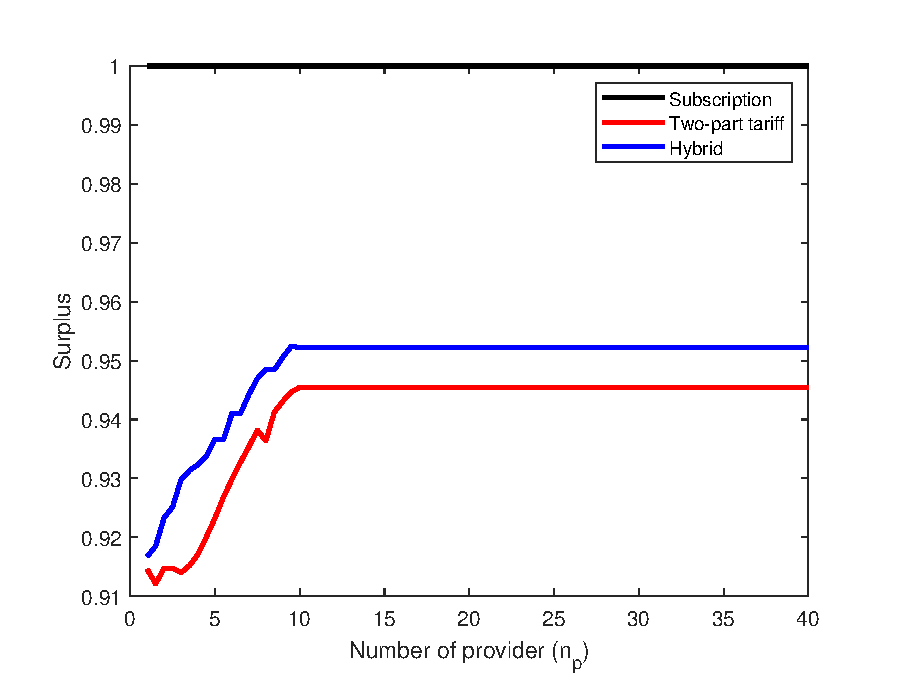
\includegraphics[width=8cm]{figure_3rd_final/f_low.eps} 
\textbf{\caption{Surplus Comparison for Extremely Low Operating Costs}}
\label{fig:app_lowxi}
\end{figure}

\subsection{Assumptions on Renters}
 
We conduct a numerical analysis for different shapes of the download frequency distribution. We vary the Pareto's shape parameter $b$ by three levels ($b=3, 4, \text{or } 5$) and present the results in \textbf{Figure \ref{fig:app_pareto}}. Here, the red (blue) line indicates the relative total surplus of the two-part tariff (the hybrid pricing) compared with the subscription-based pricing, which is represented as the horizontal black line. As suggested by our closed-form results, the total surplus of the two-part tariff and the hybrid pricing can be higher (lower) than the subscription-based pricing when the number of potential providers is small (large).

% \begin{figure}[ht!]
% \centering
% \includegraphics[width=8cm]{figure_3rd_final/f_main_modify.eps} 
% \caption{main}
% \end{figure}
%%%%%%%%%%%%%%%%%%%%%%%
\begin{figure}[ht!]
    \centering
    \subfigure[$b=3$]{\includegraphics[width=5cm]{figure_3rd_final/main_3.eps}}
    \subfigure[$b=4$]{\includegraphics[width=5cm]{figure_3rd_final/main_4.eps}}
    \subfigure[$b=5$]{\includegraphics[width=5cm]{figure_3rd_final/main_5.eps}}    
    \textbf{\caption{Numerical Analysis on Different Parameters of the Pareto Distribution.}}
    \label{fig:app_pareto}
\end{figure}

We examine whether the implications of pricing schemes are qualitatively consistent after relaxing this assumption that a renter's utility per bandwidth volume is independent of her download frequency. Specifically, we examine a scenario where potential renters with the higher utility per download volume tend to have more frequent download requests. We manipulate the shape parameter $b$ of the Pareto distribution---which determines the extent to which the bandwidth frequency is concentrated or dispersed---differently by the utility per bandwidth volume. We divide potential renters into two groups: 1) renters whose unit utility is uniformly distributed in $[0, 0.5]$ and whose frequency follows the Pareto distribution having a lighter tail (with $b_l=5$), and 2) those whose unit utility is uniformly distributed in $[0.5, 1]$ and whose frequency follows the Pareto distribution having a heavier tail (with $b_h=2$), where $b_l > b_h$. \textbf{Figure C.3} present the results for this scenario. The red (blue) line indicates the relative total surplus of the two-part tariff (the hybrid pricing) compared with the subscription-based pricing, which is represented as the horizontal black line. We observe that our main findings remain qualitatively consistent.

\begin{figure}[ht!]
\centering
\includegraphics[width=8cm]{figure_3rd_final/half_1.eps} 
\textbf{\caption{Numerical Analysis on Positive Association Between Utility per Download and Download Frequency}}
\label{fig:app_utilfreq}
\end{figure}

% R2's Points A2a (Renter's storage volume heterogeneity)
Lastly, we analyze the heterogeneity of storage demand. To do so, we redefine our utility functions to account for storage volume heterogeneity and determine renter parameters to explore.

\textbf{Generalized utility function.} Since the utility functions in our main model concern renters with a unit storage volume only, we need to define new utility functions for renters with heterogeneous storage volume. To do this, we have considered renter $i$ having storage volume $v_i$ and frequency $\lambda_i$. For this renter's utility function, we have assumed that 1) the benefit from P2P storage is proportional to $\lambda_i v_i$, 2) the storage cost is proportional to $v_i$, and 3) the bandwidth volume is $v_i$ times of the unit-volume renter with $\lambda_i$.

Based on these assumptions, we have seen that for the two-part tariff and subscription-based pricing, the new utility function is $v_i$ times of the previous function for a unit storage volume. However, the hybrid pricing might have various utility forms regarding how to price bandwidth services. For instance, the platform may offer the volume of bandwidth allowance proportionally to storage volume, which is widely observed in cloud service contracts. Also, the platform may provide the volume constantly across all renters regardless of their storage volume.

Since these possibilities seem plausible, we have examined both cases to explore the implications of hybrid pricing in the new setting. Below, we have specified the renter's utility functions in the current model and the extended ones that account for volume heterogeneity.

Here are the current utility functions of renters by pricing scheme:
\begin{equation*}
    U_i = \begin{cases}
    \lambda_i u_i - \theta p_s &\text{ under the subscription-based pricing,}\\
    \lambda_i u_i - \theta p_s - \max\{\lambda_i - q \lambda_0, 0\}p_b &\text{ under the hybrid pricing,}\\
    \lambda_i u_i - \theta p_s - \lambda_i p_b &\text{ under the two-part tariff.}
    \end{cases}
\end{equation*}
We generalize those functions for renter $i$'s storage volume $v_i$ as follows. First, when the bandwidth allowance is proportional to $v_i$, we can rewrite the functions as follows (\textbf{Utility Function I}):
\begin{equation*}
    U_i = \begin{cases}
    \lambda_i u_i v_i- \theta v_i p_s &\text{ under the subscription-based pricing,}\\
    \lambda_i u_i v_i- \theta v_i p_s - \max\{\lambda_i v_i - q \lambda_0 v_i, 0\}p_b &\text{ under the hybrid pricing,}\\
    \lambda_i u_i v_i- \theta v_i p_s - \lambda_i v_i p_b &\text{ under the two-part tariff.}
    \end{cases}
\end{equation*}
If $\lambda_0$ is independent of $v_i$, the utility is proportional to $v_i$ for all pricing schemes. Therefore, mere differences in storage demand do not affect a renter's adoption decision in this situation.

Second, we can rewrite the utility functions when the bandwidth allowance is constant as follows (\textbf{Utility Function II}): 
\begin{equation*}
    U_i = \begin{cases}
    \lambda_i u_i v_i- \theta v_i p_s &\text{ subscription}\\
    \lambda_i u_i v_i- \theta v_i p_s - \max\{\lambda_i v_i- q \lambda_0, 0\}p_b &\text{ hybrid}\\
    \lambda_i u_i v_i- \theta v_i p_s - \lambda_i v_i p_b &\text{ two-part tariff}
    \end{cases}
\end{equation*}
The notable difference is that the cost for bandwidth service in the hybrid pricing is not proportional to $v_i$. Specifically, the bandwidth fees are more burdensome for renters with high $v_i$ than those with low $v_i$. Noe that this situation is equivalent to having $v_i$ renters with a unit storage volume receives the free bandwidth allowance of $q\lambda_0 / v_i$. Therefore, the renter's decision can vary due to the storage demand.

\textbf{Renter heterogeneity.}  Considering the two types of possible utility functions, we conduct numerical studies on two renter-heterogeneity scenarios. First, we have examined the scenario where low-storage renters with storage volume ($v_l = 1$) and high-storage renters with storage volume ($v_h = 10$) have the same frequency distribution. We have set the parameters of Pareto distributions as $b_l = b_h = 2$ \textit{(\underline{Scenario i})}. Second, we have postulated that low-storage renters with storage volume ($v_l = 1$) and high-storage renters with storage volume ($v_h = 10$) have different frequency distributions. To make low-storage renters tend to request downloads more frequently than high-storage renters, we have chosen $b_l = 2$ and $b_h = 5$ for their Pareto distributions \textit{(\underline{Scenario ii})}.

To account for potential impacts of the renter composition, we have varied the proportions of low- and high-storage renters (9:1, 5:5, and 1:9) for each scenario. We have selected $q=3$ for our analysis. The results show that our findings remain consistent in all of the utility functions and scenarios (see \textbf{Figures C.4 through C.7}); that is, the total surplus of the two-part tariff (red lines) and that of the hybrid pricing (blue lines) can be higher/lower than the subscription-based pricing (normalized as 1, presented by the black horizontal line) when the number of potential providers is small/large. We find that the main insights from the basic setup remain qualitatively unchanged in our results.

%\textbf{Utility function I.} When the bandwidth allowance is proportional to a renter's storage volume

%\underline{\textit{Scenario i})} $(b_l, b_h) = (2, 2)$
%비중에 따른 3개 그래프\\
\begin{figure}[ht!]
    \centering
    \subfigure[$Low:High = 9:1$]{\includegraphics[width=5cm]{figure_3rd_final/prop_c_1.eps}}
    \subfigure[$Low:High = 5:5$]{\includegraphics[width=5cm]{figure_3rd_final/prop_c_2.eps}}
    \subfigure[$Low:High = 1:9$]{\includegraphics[width=5cm]{figure_3rd_final/prop_c_3.eps}}    
    \textbf{\caption{Numerical Analysis for Utility Function I and Scenario \textit{i}}}
\end{figure} 

%\underline{\textit{Scenario ii})} $(b_l, b_h) = (2, 5)$
\begin{figure}[ht!]
    \centering
    \subfigure[$Low:High = 9:1$]{\includegraphics[width=5cm]{figure_3rd_final/prop_c_4_1.eps}}
    \subfigure[$Low:High = 5:5$]{\includegraphics[width=5cm]{figure_3rd_final/prop_c_5_1.eps}}
    \subfigure[$Low:High = 1:9$]{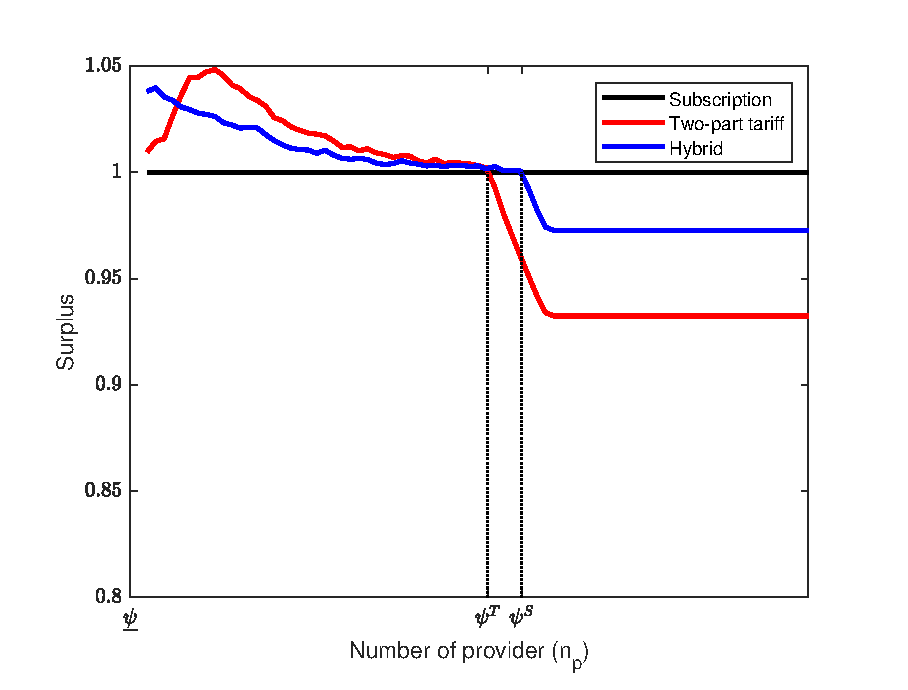
\includegraphics[width=5cm]{figure_3rd_final/prop_c_6_1.eps}}
    \textbf{\caption{Numerical Analysis for Utility Function I and Scenario \textit{ii}}}
\end{figure}
%- 아래의 pareto distribution에서 parameter가 달라질 때 효과와 연결\\
%- 용량이 큰 고객의 $b$가 큰 경우에, 이들에게는 i) first-best 인 부분에서 bandwidth에 비용을 지불받는 것의 merit이 줄어들어 subscription과 가까워짐 2) 마찬가지로 market-clearing에서도 bandwidth로부터 얻는 이익이 많이 없어져서 subscription과 가까워짐 -- c로 갈 수록 전체적으로 subscription과 가까워지는 모습(특히, hybrid)\\

%\textbf{Utility function II.}  When the bandwidth allowance is constant
\newpage
%\underline{\textit{Scenario i})} $(b_l, b_h) = (2, 2)$
\begin{figure}[ht!]
    \centering
    \subfigure[$Low:High = 9:1$]{\includegraphics[width=5cm]{figure_3rd_final/volume_c_1.eps}}
    \subfigure[$Low:High = 5:5$]{\includegraphics[width=5cm]{figure_3rd_final/volume_c_2.eps}}
    \subfigure[$Low:High = 1:9$]{\includegraphics[width=5cm]{figure_3rd_final/volume_c_3.eps}}
    \textbf{\caption{Numerical Analysis for Utility Function II and Scenario \textit{i}}}
\end{figure}

%\underline{\textit{Scenario ii})} $(b_l, b_h) = (2, 5)$
%%%%%%%%%%%%%%%%%%
\begin{figure}[ht!]
    \centering
    \subfigure[$Low:High = 9:1$]{\includegraphics[width=5cm]{figure_3rd_final/volume_c_4.eps}}
    \subfigure[$Low:High = 5:5$]{\includegraphics[width=5cm]{figure_3rd_final/volume_c_5.eps}}
    \subfigure[$Low:High = 1:9$]{\includegraphics[width=5cm]{figure_3rd_final/volume_c_6.eps}}
    \textbf{\caption{Numerical Analysis for Utility Function II and Scenario \textit{ii}}}
\end{figure}



\end{document}